\documentclass[aps,prd,twocolumn,nofootinbib,superscriptaddress,floatfix]{revtex4-2}

\usepackage{amsmath,amssymb}
\usepackage{graphicx}
\usepackage{bm}
\usepackage{xcolor}
\usepackage[colorlinks=true,linkcolor=blue!60!black,citecolor=blue!60!black,urlcolor=blue!60!black]{hyperref}

\graphicspath{{figures/}}

% Notation
\newcommand{\Hp}{\mathcal{H}}
\newcommand{\dd}{\mathrm{d}}
\newcommand{\Mpc}{\,\mathrm{Mpc}}
\newcommand{\hMpc}{\,h\,\mathrm{Mpc}^{-1}}
\newcommand{\Om}{\Omega}
\newcommand{\gt}{\tilde g}
\newcommand{\muK}{\,\mu\mathrm{K}^2}

\begin{document}

\title{A line-of-sight Einstein--Boltzmann solver for the CMB and the matter power spectrum}

\author{H. A. Winther}
\email{h.a.winther@astro.uio.no}
\affiliation{Institute of Theoretical Astrophysics, University of Oslo, P.O.~Box 1029 Blindern, N-0315 Oslo, Norway}

\date{\today}

\begin{abstract}
We describe a new C++ Einstein--Boltzmann code that computes the angular power spectra of the cosmic microwave
background (CMB) temperature and $E$-mode polarization, and the linear matter power spectrum, for a flat
$\Lambda$CDM model. The calculation is split into four modules: the background expansion, the recombination
history, the linear perturbations, and the line-of-sight integration. The code includes photon polarization, massless
neutrinos, helium and a tanh model of reionization. For the fiducial model ($h=0.67$, $\Om_{b}=0.05$,
$\Om_{\rm CDM}=0.267$) we find radiation--matter equality at $z=3400$, an age of $13.85$\,Gyr and last scattering
at $z_*=1085$ (with reionization; $1090$ without) with sound horizon $r_s(z_*)=144.9\Mpc$. The first acoustic peak
lies at $\ell=221$ and $P(k)$ peaks at $k=0.0167\hMpc$. Every module agrees with the CLASS code run with the same
physics, the TT spectrum to better than $1.1\%$ for $2\le\ell\le2000$ and $P(k)$ to $0.11\%$. The unlensed TT spectrum
matches the shape of the Planck 2018 data, and the residuals at $\ell\gtrsim 1000$ follow the pattern expected from
gravitational lensing. Including lensing with the full-sky correlation-function method lowers the $\chi^2$ against
the 83 binned Planck high-$\ell$ points from 781 to 220; the lensed TT agrees with CLASS to $10^{-3}$ for $\ell\le2000$. We also show that supernova distances alone prefer
$h\simeq0.70$ when the density parameters are held fixed. Finally, we extend the code to open and closed universes
using hyperspherical Bessel functions; for $|\Om_K|\le0.2$ the spectra agree with CLASS as well as in the flat case.
We also add a massive neutrino species; the suppression of the matter power spectrum (16\% at $k=0.5\hMpc$ for
$m_\nu=0.3$\,eV) and of the lensing potential agree with CLASS to $5\times10^{-4}$. Finally, we compute the real-space two-point
functions: the CMB angular correlation functions, the matter correlation function with its BAO peak at
$100\,h^{-1}\Mpc$, and the angular power spectrum and correlation function of the matter projected over a redshift
distribution, which agree with CLASS to $2\times10^{-3}$. Replacing the Peebles recombination model by RECFAST
reduces the rms differences from CLASS to 0.048\% in TT and
0.32\% in EE for $30\le\ell\le1000$. Lastly, we describe a library of eleven
dark-energy and modified-gravity models: quintessence, coupled quintessence, dark scattering, early dark energy,
interacting dark energy, $\mu$--$\Sigma$, DGP, Brans--Dicke, $f(R)$, the cubic Galileon, and Horndeski gravity in the
$\alpha$ basis. They are validated with constraint equations, independent growth calculations and reconstructions of
one theory from another, and against CLASS, hi\_class and CLASS\_EDE where these apply.
\end{abstract}

\maketitle

% ===========================================================================
\section{Introduction}
% ===========================================================================

The anisotropies of the CMB and the clustering of matter on large scales are the two cleanest probes of the
early Universe. Both are set by linear physics. Small primordial curvature fluctuations, generated during inflation,
evolve under gravity and under photon--baryon interactions. The result is a set of transfer functions that map the
primordial spectrum onto the observed spectra. Computing these transfer functions is the job of an
Einstein--Boltzmann solver. Public codes such as CMBFAST~\cite{Seljak1996}, CAMB~\cite{Lewis2000} and
CLASS~\cite{Lesgourgues2011,Blas2011} do this to sub-percent precision and are the basis of all modern parameter
estimates, including those of Planck~\cite{Planck2018params}.

This paper describes the four milestones of writing such a code from scratch. The structure follows the physics:
\begin{enumerate}
\item \textbf{Background cosmology} (Sec.~\ref{sec:m1}): the expansion history $H(x)$, conformal time and distances.
      We test it against supernova data.
\item \textbf{Recombination history} (Sec.~\ref{sec:m2}): the free electron fraction $X_e$, the optical depth $\tau$
      and the visibility function $\gt$, which decide when and where CMB photons last scatter.
\item \textbf{Perturbations} (Sec.~\ref{sec:m3}): the linearized Einstein and Boltzmann equations for dark matter,
      baryons, photons (temperature and polarization) and massless neutrinos, solved for each Fourier mode $k$.
\item \textbf{Power spectra} (Sec.~\ref{sec:m4}): the line-of-sight integration~\cite{Seljak1996} that gives the
      photon transfer functions $\Theta_\ell(k)$ and the angular spectra $C_\ell^{TT}$, $C_\ell^{EE}$, $C_\ell^{TE}$,
      together with the matter power spectrum $P(k)$.
\end{enumerate}
Each module is a separate C++ class that takes the previous one as input. Each section below gives the theory, the
implementation and tests, and the results for one milestone. Sec.~\ref{sec:validation} compares all modules with CLASS,
and Sec.~\ref{sec:conclusions} concludes. The course project also includes Markov chain Monte Carlo (MCMC) fits of
supernova data; as instructed, these are omitted here.

Throughout we use the time variable $x=\ln a$, the conformal Hubble factor $\Hp=aH$, and primes for derivatives with
respect to $x$. The perturbations use the conformal Newtonian gauge and the conventions of
Callin~\cite{Callin2006} and Dodelson~\cite{Dodelson2003}. Internally the code works in SI units.

The fiducial model is $h=0.67$, $\Om_{b0}=0.05$, $\Om_{\rm CDM0}=0.267$, $\Om_{K0}=0$, $T_{\rm CMB}=2.7255$\,K,
$N_{\rm eff}=3.046$, $Y_p=0.245$, reionization at $z_{\rm re}=8$ ($\Delta z=0.5$) and helium reionization at
$z=3.5$ ($\Delta z=0.5$), with primordial amplitude $A_s=2.1\times10^{-9}$ and tilt $n_s=0.965$ at
$k_{\rm pivot}=0.05\Mpc^{-1}$. $\Om_{\Lambda0}$ is fixed by flatness.

% ===========================================================================
\section{Milestone I: The background cosmology}\label{sec:m1}
% ===========================================================================

The first milestone computes the expansion history of a homogeneous and isotropic Universe. Every later module
needs it: the recombination rates are set by the competition between atomic reaction rates and the expansion rate
$H$, the perturbation equations contain $\Hp$ and its derivatives, and the line-of-sight integral needs the conformal
distance $\eta_0-\eta$ to the last-scattering surface. The background also contains the first test of the model
against data, through the distances to type Ia supernovae.

\subsection{Theory}

\paragraph*{The metric and the Friedmann equations.} The cosmological principle states that on large scales the
Universe is homogeneous and isotropic. The most general metric with these symmetries is the
Friedmann--Lema\^itre--Robertson--Walker (FLRW) metric,
\begin{equation}
\dd s^2 = -c^2\dd t^2 + a^2(t)\Big[\frac{\dd r^2}{1-kr^2} + r^2\dd\Omega^2\Big],
\end{equation}
where $r$ is a comoving radial coordinate, $k$ is the spatial curvature and $a(t)$, normalized to $a(t_0)=1$ today,
is the scale factor. All the dynamics is in $a(t)$. Because of the symmetry, the matter content must be a set of
perfect fluids with energy density $\rho_i c^2$ and pressure $P_i=w_i\rho_ic^2$. Inserting the metric and fluids in
Einstein's equations gives two independent equations. The $00$ component is the Friedmann equation,
\begin{equation}
H^2\equiv\Big(\frac{\dot a}{a}\Big)^2 = \frac{8\pi G}{3}\sum_i\rho_i - \frac{kc^2}{a^2},
\label{eq:friedmann}
\end{equation}
and the trace of the $ij$ components gives the acceleration equation,
\begin{equation}
\frac{\ddot a}{a} = -\frac{4\pi G}{3}\sum_i\Big(\rho_i+\frac{3P_i}{c^2}\Big).
\label{eq:accel}
\end{equation}
Combining them gives energy conservation, $\dot\rho_i+3H(\rho_i+P_i/c^2)=0$, which for constant $w_i$ integrates to
$\rho_i\propto a^{-3(1+w_i)}$. The relevant cases are:
\begin{itemize}
\item Non-relativistic matter (baryons and cold dark matter), $w=0$. The number of particles in a comoving volume is
      conserved, so $\rho_M\propto a^{-3}$.
\item Radiation (photons and massless neutrinos), $w=1/3$. The number density falls as $a^{-3}$ and, in addition, every
      particle loses energy to the redshift, $E\propto a^{-1}$, so $\rho_r\propto a^{-4}$.
\item A cosmological constant, $w=-1$, with $\rho_\Lambda$ constant: the vacuum energy per volume does not dilute.
\end{itemize}
Curvature enters Eq.~\eqref{eq:friedmann} like a fluid with $\rho\propto a^{-2}$. Dividing by $H_0^2$ and defining
the density parameters relative to the critical density $\rho_{c0}=3H_0^2/8\pi G$ (the density of a flat universe),
$\Om_{i0}=\rho_{i0}/\rho_{c0}$ and $\Om_{K0}=-kc^2/H_0^2$, gives
\begin{equation}
H(x) = H_0\sqrt{\Om_{M0}e^{-3x} + \Om_{r0}e^{-4x} + \Om_{K0}e^{-2x} + \Om_{\Lambda0}} ,
\label{eq:H}
\end{equation}
where $\Om_M=\Om_b+\Om_{\rm CDM}$ and $\Om_r=\Om_\gamma+\Om_\nu$. We use $x=\ln a$ as time variable. The interesting
history spans some twenty $e$-folds of expansion, and most quantities vary as powers of $a$, which are simple
exponentials in $x$. Evaluating Eq.~\eqref{eq:H} today gives the constraint $\sum_i\Om_{i0}=1$, which fixes
$\Om_{\Lambda0}$ in a flat universe. The density parameters at other times are
$\Om_i(x)=\Om_{i0}e^{-n_ix}H_0^2/H^2(x)$, with $n_i=3,4,2,0$ for matter, radiation, curvature and $\Lambda$; they
measure which component drives the expansion at a given time.

\paragraph*{The radiation density.} The CMB is a blackbody with temperature $T_{\rm CMB}=2.7255$\,K, so its density
follows from the Stefan--Boltzmann law: integrating the Bose--Einstein distribution over momenta, with two
polarization states, gives $\rho_\gamma c^2=2\cdot\frac{\pi^2}{30}(k_BT)^4/(\hbar c)^3$ and
\begin{equation}
\Om_{\gamma0} = 2\cdot\frac{\pi^2}{30}\frac{(k_BT_{\rm CMB})^4}{\hbar^3c^5}\cdot\frac{8\pi G}{3H_0^2}.
\end{equation}
Neutrinos decoupled from the plasma at $T\sim1$\,MeV, just before electrons and positrons annihilated. The annihilation
heated the photons but not the neutrinos, and entropy conservation gives $T_\nu=(4/11)^{1/3}T_\gamma$ afterwards.
Fermions also carry a factor $7/8$ relative to bosons in the energy density. With $N_{\rm eff}$ species,
$\Om_{\nu0}=N_{\rm eff}\,\tfrac{7}{8}(4/11)^{4/3}\Om_{\gamma0}$. $N_{\rm eff}=3.046$ rather than 3 because the
neutrinos were still slightly coupled when the annihilation began and shared a little of its energy.

\paragraph*{Clocks and horizons.} Cosmic time $t$ is the time measured by an observer at rest with respect to the
expansion. Conformal time $\eta$ is defined by $c\,\dd t=a\,\dd\eta$, so that light moves on straight lines in
$(\eta,\chi)$ coordinates with $\dd\chi=c\,\dd\eta$. In terms of $x$,
\begin{equation}
\frac{\dd t}{\dd x} = \frac{1}{H}, \qquad \frac{\dd\eta}{\dd x} = \frac{c}{\Hp},\qquad \Hp\equiv aH=\dot a.
\label{eq:eta}
\end{equation}
$\eta(x)$ is the comoving distance light has travelled since the Big Bang, the \emph{particle horizon}. Two regions
farther apart than $\eta$ have never been in causal contact. The quantity $c/\Hp$ is the comoving Hubble radius, the
distance over which the expansion velocity reaches $c$, and over which causal physics can act within one expansion
time. A perturbation of comoving wavenumber $k$ is outside the horizon when $ck<\Hp$ and inside when $ck>\Hp$. In a
decelerating universe ($\ddot a<0$) $\Hp=\dot a$ decreases, so ever larger scales enter the horizon. This is central
for the perturbations of Milestone~III.

\paragraph*{Single-component limits.} If one component with $\rho\propto a^{-n}$ dominates, then
$\Hp\propto a^{1-n/2}=e^{-(n-2)x/2}$, and Eq.~\eqref{eq:eta} gives $\eta=2c/[(n-2)\Hp]$ for $n>2$. Hence
\begin{equation}
\frac{\Hp'}{\Hp}=1-\frac{n}{2},\qquad \frac{\Hp''}{\Hp}=\Big(1-\frac{n}{2}\Big)^2,\qquad \frac{\eta\Hp}{c}=\frac{2}{n-2},
\label{eq:Hp_limits}
\end{equation}
that is $(-1,1,1)$ in radiation domination (RD) and $(-\tfrac12,\tfrac14,2)$ in matter domination (MD). In $\Lambda$
domination $H$ is constant, $\Hp\propto a$, $\Hp'/\Hp=\Hp''/\Hp=1$, and $\eta$ approaches a finite value: there is an
event horizon, and we will never see beyond it. The corresponding laws for cosmic time are $t\propto a^2$ (RD),
$t\propto a^{3/2}$ (MD) and $t\propto\ln a$ ($\Lambda$). These limits are our main tests.

\paragraph*{Distances.} Light from an object at $x$ has travelled a comoving distance $\chi=\eta_0-\eta(x)$. In a
curved universe the comoving \emph{transverse} distance is $r=\chi\,\mathrm{sinn}(\sqrt{|\Om_{K0}|}H_0\chi/c)/
(\sqrt{|\Om_{K0}|}H_0\chi/c)$, with $\mathrm{sinn}=\sinh$ for $\Om_{K0}>0$ and $\sin$ for $\Om_{K0}<0$; for flat space
$r=\chi$. An object of physical size $D$ at scale factor $a$ subtends the angle $\theta=D/(ar)$, so the angular
diameter distance is $d_A=ar$. A source of luminosity $L$ spreads its light over a sphere of comoving area $4\pi r^2$,
and each photon arrives with its energy reduced by $(1+z)$ and its arrival rate reduced by another $(1+z)$ because of
time dilation. The flux is then $F=L/(4\pi d_L^2)$ with the luminosity distance $d_L=r/a=(1+z)^2d_A$.

At low redshift $d_L\simeq cz/H_0$, Hubble's law. The next term,
$d_L\simeq(cz/H_0)[1+\tfrac12(1-q_0)z]$, depends on the deceleration parameter $q_0=-\ddot a/(aH^2)|_0=
\tfrac12\Om_{M0}-\Om_{\Lambda0}$ (neglecting radiation). In an accelerating universe ($q_0<0$) distant objects are
farther away, and therefore fainter, than in a decelerating one. This is how supernovae revealed the accelerated
expansion.

\paragraph*{Key epochs.} Three epochs are of special interest:
\begin{itemize}
\item Radiation--matter equality, $\rho_r=\rho_M$, at $a_{\rm eq}=\Om_{r0}/\Om_{M0}$.
\item Matter--$\Lambda$ equality at $a^3=\Om_{M0}/\Om_{\Lambda0}$.
\item The onset of acceleration, $\ddot a=0$. Equation~\eqref{eq:accel} shows that a component accelerates the
      expansion only if $w<-1/3$. Matter contributes $\rho_M$ and $\Lambda$ contributes $\rho_\Lambda+3P_\Lambda/c^2=
      -2\rho_\Lambda$, so acceleration starts when $\rho_M=2\rho_\Lambda$, i.e.\ $\Om_{M0}a^{-3}=2\Om_{\Lambda0}$.
      Since $\ddot a=\dot\Hp$, this is also where $\Hp'=0$.
\end{itemize}
The wavenumber that enters the horizon at equality, $k_{\rm eq}=\Hp(x_{\rm eq})/c$, separates modes that entered
during RD from those that entered during MD. It sets the turnover scale of $P(k)$ (Sec.~\ref{sec:m4}).

\subsection{Implementation and tests}

\texttt{BackgroundCosmology} writes $E^2=H^2/H_0^2$ as a sum of virtual component densities, each with analytic first
and second $x$-derivatives. $\Hp$, $\Hp'$ and $\Hp''$ are therefore analytic. A new model, for example dynamical dark
energy, only overrides the density of one component; the code includes a CPL $w_0w_a$ example. We solve
Eq.~\eqref{eq:eta} on $x\in[-20,5]$ with an adaptive Runge--Kutta (RK8PD) solver and store $\eta$ and $t$ in cubic
splines. The initial values come from the exact solution for a universe with radiation and matter only,
\begin{equation}
\eta = \frac{2ca}{H_0\big(\sqrt{\Om_{r0}+\Om_{M0}a}+\sqrt{\Om_{r0}}\big)},
\end{equation}
which is exact up to the negligible $\Lambda$ term at $x=-20$; the analogous expression is used for $t$. The epochs
are found by root finding on the analytic expressions.

Figure~\ref{fig:Hp_tests} shows the two standard tests. $\Hp'/\Hp$ and $\Hp''/\Hp$ reach the plateaus of
Eq.~\eqref{eq:Hp_limits} in each era, with smooth transitions at the equality epochs. $\eta\Hp/c$ goes from 1 in RD
towards 2 in MD. It never quite reaches 2: matter domination is too short, and $\eta$ still remembers the radiation
era when $\Lambda$ takes over. In the $\Lambda$ era $\eta$ freezes while $\Hp$ grows, so $\eta\Hp/c$ increases. The
derivative of the $\eta$ spline satisfies $\eta'\Hp/c=1$ to $\max|\eta'\Hp/c-1|=9.8\times10^{-6}$, which checks both
the ODE and the spline. The unit tests also check $t$ against the analytic Einstein--de Sitter result, the analytic
derivatives against finite differences, and $\eta$ against an independent quadrature. Section~\ref{sec:validation}
shows that $H$, $t$ and $\eta$ agree with CLASS to $\sim10^{-7}$.

\begin{figure}
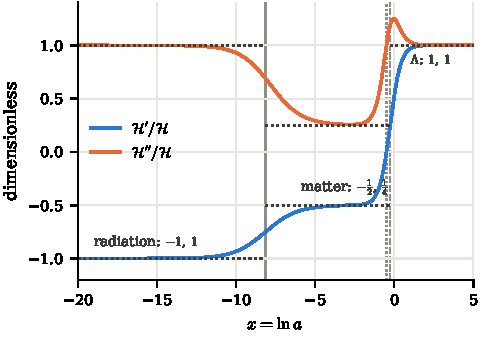
\includegraphics[width=\columnwidth]{m1_Hp_derivatives}
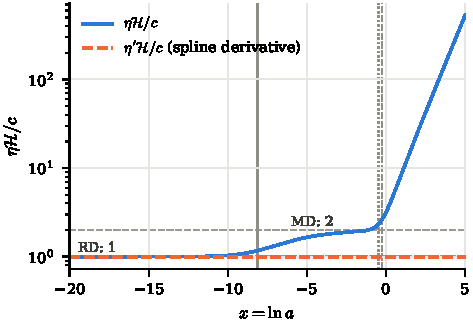
\includegraphics[width=\columnwidth]{m1_etaHp}
\caption{Tests of the background. \emph{Top:} $\Hp'/\Hp$ and $\Hp''/\Hp$. The short dotted lines are the analytic
values of Eq.~\eqref{eq:Hp_limits} in the radiation, matter and $\Lambda$ eras. \emph{Bottom:} $\eta\Hp/c$, which is
1 in RD and approaches 2 in MD, and $\eta'\Hp/c$ from the derivative of the spline, which should be exactly 1. In all
Milestone~I figures the vertical lines mark radiation--matter equality (solid), matter--$\Lambda$ equality (dashed) and
the onset of acceleration (dotted).}
\label{fig:Hp_tests}
\end{figure}

\subsection{Results}

The expansion history is shown in Figs.~\ref{fig:Hp}--\ref{fig:Omegas} and the key epochs are listed in
Table~\ref{tab:m1}.

\paragraph*{The three eras.} Figure~\ref{fig:Omegas} shows the succession of eras that follows from the different
dilution laws. Going back in time, radiation ($\propto a^{-4}$) eventually wins over matter ($\propto a^{-3}$), which
in turn wins over the constant $\rho_\Lambda$. Radiation dominates until $z=3400$, when the Universe was only
$51\,000$ years old. Matter then dominates for most of cosmic history, and $\Lambda$ only takes over at $z=0.29$. Before
$z\sim2$ the cosmological constant is completely negligible; that we happen to live just when $\Om_M$ and $\Om_\Lambda$
are comparable is the so-called coincidence problem. Today $\Om_{\Lambda0}=0.6829$, $\Om_{\gamma0}=5.51\times10^{-5}$
and $\Om_{\nu0}=3.81\times10^{-5}$.

\paragraph*{The conformal Hubble factor.} $\Hp$ (Fig.~\ref{fig:Hp}) falls as $e^{-x}$ in RD and as $e^{-x/2}$ in MD,
exactly as Eq.~\eqref{eq:Hp_limits} predicts. Because $\Hp=\dot a$, its slope is the sign of the acceleration: $\Hp$
has a minimum exactly at the onset of acceleration, $z=0.627$, and then grows as $e^{x}$. Acceleration starts well
before matter--$\Lambda$ equality at $z=0.292$, because the pressure of the cosmological constant counts twice in
Eq.~\eqref{eq:accel}: $\Lambda$ only needs half the matter density to make $\ddot a>0$. A falling $\Hp$ means the
comoving Hubble radius $c/\Hp$ grows and new scales enter the horizon; after $z=0.63$ this has reversed, and scales
are now leaving the horizon again.

\paragraph*{Age and horizon.} The age of the Universe is $t_0=13.85$\,Gyr (Fig.~\ref{fig:times}). This is
$0.949\,H_0^{-1}$, with $H_0^{-1}=14.59$\,Gyr. A flat matter-only (Einstein--de Sitter) universe with the same $H_0$
would be only $\tfrac23H_0^{-1}=9.7$\,Gyr old, younger than the oldest stars. The cosmological constant slowed the
expansion less in the past, so it took longer to reach today's expansion rate, and the Universe is older. The
conformal time today is $\eta_0/c=46.29$\,Gyr ($\eta_0=14\,192\Mpc=3.17\,c/H_0$). This is the comoving radius of the
observable Universe: light has travelled for 13.85\,Gyr, but the space it crossed has expanded in the meantime.

The radiation era is short in cosmic time but long in conformal time, because $\dd\eta=c\,\dd t/a$ weighs early times
by $1/a$. About $40\%$ of the conformal time at recombination accumulates before equality. The comoving horizon at
recombination is $\eta_*\approx280\Mpc$, only $2\%$ of the distance $\eta_0-\eta_*$ to the last-scattering surface. It
subtends an angle of about $1^\circ$ on the sky. Regions of the CMB separated by more than this were causally
disconnected at recombination, which is the horizon problem that inflation is invoked to solve. It is also why the
acoustic features of the CMB appear at $\ell\sim200$ (Sec.~\ref{sec:m4}).

\begin{table}
\caption{Key epochs of the fiducial background. The ages are cosmic times since the Big Bang.}
\label{tab:m1}
\begin{ruledtabular}
\begin{tabular}{lccc}
Event & $x$ & $z$ & $t$ \\
\hline
Radiation--matter equality & $-8.1319$ & $3400.3$ & $51\,029$\,yr \\
Onset of acceleration       & $-0.4865$ & $0.6267$ & $7.750$\,Gyr \\
Matter--$\Lambda$ equality  & $-0.2558$ & $0.2915$ & $10.371$\,Gyr \\
Today                       & $0$       & $0$      & $13.848$\,Gyr \\
\end{tabular}
\end{ruledtabular}
\end{table}

\begin{figure}
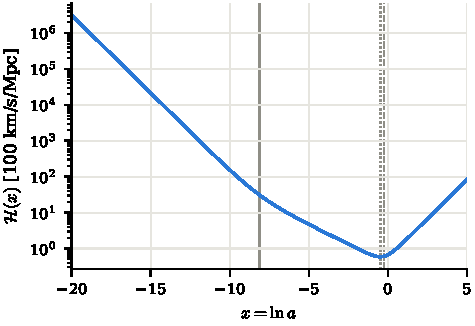
\includegraphics[width=\columnwidth]{m1_Hp}
\caption{The conformal Hubble factor $\Hp=aH=\dot a$ in units of $100$\,km\,s$^{-1}$\,Mpc$^{-1}$. It decreases during
RD and MD, when the expansion decelerates, and increases after the onset of acceleration (dotted line).}
\label{fig:Hp}
\end{figure}

\begin{figure}
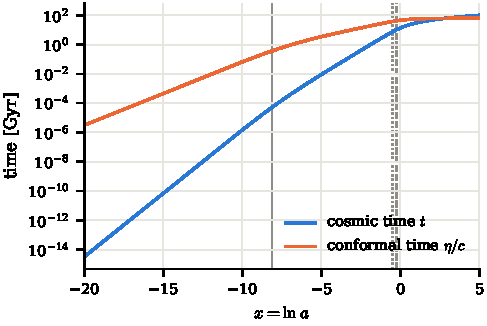
\includegraphics[width=\columnwidth]{m1_times}
\caption{Cosmic time $t$ and conformal time $\eta/c$ in Gyr. In RD $t\propto a^2$ and $\eta\propto a$; in MD
$t\propto a^{3/2}$ and $\eta\propto a^{1/2}$. $\eta$ freezes at $\eta_0/c=46.3$\,Gyr in the $\Lambda$ era, while $t$
grows logarithmically in $a$.}
\label{fig:times}
\end{figure}

\begin{figure}
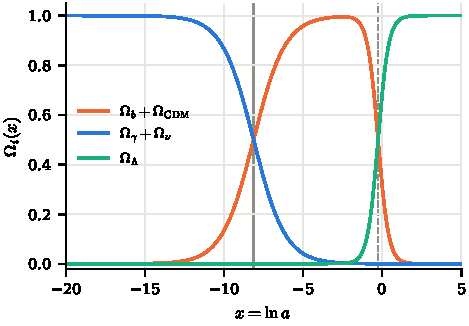
\includegraphics[width=\columnwidth]{m1_Omegas}
\caption{Density parameters of relativistic species ($\Om_\gamma+\Om_\nu$), matter ($\Om_b+\Om_{\rm CDM}$) and dark
energy ($\Om_\Lambda$) as functions of $x$. They always sum to one in a flat universe.}
\label{fig:Omegas}
\end{figure}

\paragraph*{Supernovae.} Type Ia supernovae are standardizable candles: after empirical corrections for light-curve
width and colour, their peak luminosities are nearly the same. Their fluxes therefore measure $d_L(z)$.
Figure~\ref{fig:sn} compares our luminosity distance with the binned JLA distances of Betoule et
al.~\cite{Betoule2014}, plotted as $d_L/z$. At low redshift $d_L/z\to c/H_0$, and the rise with $z$ measures
$1-q_0$. Our model has $q_0=-0.52$.

The fiducial model reproduces the shape of $d_L(z)$ but is about $4\%$ too far away at all redshifts, giving
$\chi^2=141.7$ for $N=31$ points. With the density parameters fixed, $d_L\propto1/h$ and $h$ only rescales the curve.
The best fit is then $h=0.699$ with $\chi^2=30.7$, a good fit. The data clearly require acceleration. For comparison,
the best fit of a flat matter-only universe (EdS, $q_0=+\frac12$) gives $\chi^2=317$, and even an empty, coasting
universe ($q_0=0$) gives $\chi^2=49$.

The preference for $h\approx0.70$ should not be read as a measurement of $H_0$. Supernovae measure \emph{relative}
distances. The absolute scale of the data comes from the absolute magnitude adopted when converting the distance
moduli to $d_L$, which is degenerate with $H_0$. A joint fit of $h$, $\Om_{M0}$ and $\Om_{K0}$ by MCMC is part of the
course project but omitted here.

\begin{figure}
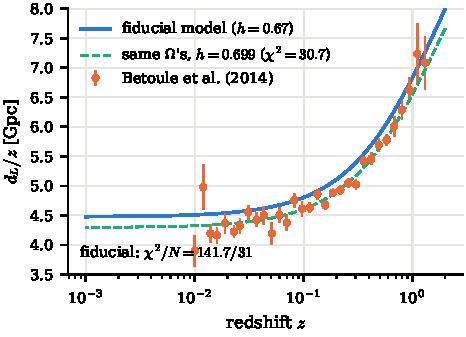
\includegraphics[width=\columnwidth]{m1_supernovae}
\caption{Luminosity distance divided by redshift for the fiducial model (solid), and for the same density parameters
with the best-fit $h$ (dashed), compared with the binned JLA supernova data~\cite{Betoule2014}. The intercept at $z\to0$
is $c/H_0$; the slope measures the acceleration of the expansion.}
\label{fig:sn}
\end{figure}

% ===========================================================================
\section{Milestone II: The recombination history}\label{sec:m2}
% ===========================================================================

Before recombination the Universe is filled with a plasma of photons, free electrons and nuclei. Thomson scattering off
the free electrons is so frequent that a photon travels only a tiny distance between collisions, and photons and
baryons move together as a single fluid. When the Universe has cooled enough for electrons to bind into neutral atoms,
the scattering stops: the photons decouple and stream freely towards us as the CMB. This milestone computes the free
electron fraction $X_e(x)$, and from it the optical depth $\tau$ and the visibility function $\gt$, which tells us
where the CMB photons last scattered.

\subsection{Theory}

We define $X_e=n_e/n_H$, where $n_H=(1-Y_p)\rho_b/m_H\propto a^{-3}$ is the number density of hydrogen nuclei, free or
bound, and $Y_p$ is the primordial helium mass fraction. Helium contributes $f_{\rm He}=n_{\rm He}/n_H=Y_p/[4(1-Y_p)]$
nuclei per hydrogen nucleus, so fully ionized hydrogen and helium give $X_e=1+2f_{\rm He}$.

\paragraph*{Saha equilibrium.} At early times the reaction $e^-+p\leftrightarrow{\rm H}+\gamma$ runs much faster than
the expansion and is in chemical equilibrium, $\mu_e+\mu_p=\mu_{\rm H}$ (photons have $\mu_\gamma=0$). The particles are
non-relativistic and non-degenerate, so each species has the Maxwell--Boltzmann density
$n_i=g_i(m_ik_BT/2\pi\hbar^2)^{3/2}e^{(\mu_i-m_ic^2)/k_BT}$. In the ratio $n_en_p/n_{\rm H}$ the chemical potentials
cancel, and the mass difference $m_e+m_p-m_{\rm H}=\epsilon_0/c^2$ leaves the binding energy $\epsilon_0=13.6$\,eV. With
$F=(m_ek_BT_b/2\pi\hbar^2)^{3/2}$ this gives the Saha equation. The same argument applies to the two ionization stages of
helium:
\begin{align}
\frac{n_e x_{\rm H^+}}{1-x_{\rm H^+}} &= F e^{-\epsilon_0/k_BT_b}, \label{eq:saha}\\
\frac{n_e x_{\rm He^+}}{x_{\rm He^0}} &= 4F e^{-\chi_0/k_BT_b},\qquad
\frac{n_e x_{\rm He^{++}}}{x_{\rm He^+}} = F e^{-\chi_1/k_BT_b}.\nonumber
\end{align}
Here $\chi_0=24.59$\,eV and $\chi_1=54.4$\,eV are the helium ionization energies, and the factors $4$ and $1$ are the
ratios of the spin degeneracies. The electron density
$n_e=n_H[x_{\rm H^+}+f_{\rm He}(x_{\rm He^+}+2x_{\rm He^{++}})]$ closes the system. For hydrogen alone,
Eq.~\eqref{eq:saha} is a quadratic in $X_e$.

Equation~\eqref{eq:saha} explains why recombination happens so late. Writing $n_e=X_en_H$ and $n_H\propto\eta_bn_\gamma$,
with $\eta_b\approx6\times10^{-10}$ baryons per photon, the right-hand side divided by $n_H$ is of order
$\eta_b^{-1}(k_BT/m_ec^2)^{3/2}e^{-\epsilon_0/k_BT}$. The huge factor $\eta_b^{-1}$ keeps hydrogen ionized until the
exponential has become very small, i.e.\ until $\epsilon_0/k_BT\approx40$--$50$. Physically, there are so many photons
per atom that even the far Wien tail of the Planck spectrum, above $13.6$\,eV, contains enough photons to ionize every
atom that forms.

\paragraph*{Peebles equation.} As $X_e$ drops, the rates fall below the expansion rate and equilibrium can no longer
be maintained. Recombination is moreover not a single-step process. A direct recombination to the ground state emits a
photon above $13.6$\,eV, which is immediately absorbed by a neighbouring atom and ionizes it again; such recombinations
achieve nothing. Recombination to an excited state cascades down to $n=2$. From $2p$ the atom emits a Lyman-$\alpha$
photon, but the Universe is extremely optically thick to Lyman-$\alpha$, so the photon is reabsorbed and the atom is
re-excited. Only two routes lead permanently to the ground state:
\begin{itemize}
\item the slow two-photon decay $2s\to1s$, with rate $\Lambda_{2s\to1s}=8.227\,{\rm s}^{-1}$;
\item the redshifting of a Lyman-$\alpha$ photon out of the line by the expansion, with rate $\Lambda_\alpha$.
\end{itemize}
Meanwhile the $n=2$ state, bound by only $\epsilon_0/4=3.4$\,eV, is easily photoionized again. Peebles' effective
three-level atom~\cite{Peebles1968} captures this physics:
\begin{equation}
\frac{\dd X_e}{\dd x} = \frac{C_r(T_b)}{H}\Big[\beta(T_b)(1-X_e) - n_H\alpha^{(2)}(T_b)X_e^2\Big].
\label{eq:peebles}
\end{equation}
The terms are as follows:
\begin{itemize}
\item The second term in the bracket is recombination. Its rate per hydrogen atom is $n_e\alpha^{(2)}$, where
      $\alpha^{(2)}$ is the case-B recombination coefficient. It counts only captures to $n\ge2$, the ones that can
      eventually lead to a neutral atom.
\item The first term is photoionization. Its rate $\beta$ follows from $\alpha^{(2)}$ by detailed balance,
      $\beta=\alpha^{(2)}Fe^{-\epsilon_0/k_BT_b}$, so that the bracket vanishes in Saha equilibrium. The rate out of
      $n=2$ is $\beta^{(2)}=\beta e^{3\epsilon_0/4k_BT_b}$.
\item The factor
\begin{equation}
C_r = \frac{\Lambda_{2s\to1s}+\Lambda_\alpha}{\Lambda_{2s\to1s}+\Lambda_\alpha+\beta^{(2)}},\quad
\Lambda_\alpha = \frac{H(3\epsilon_0)^3}{(8\pi)^2(\hbar c)^3 n_{1s}},
\end{equation}
      with $n_{1s}=(1-X_e)n_H$, is the probability that an atom in $n=2$ reaches the ground state before it is ionized
      again.
\end{itemize}
Early on $\beta^{(2)}\gg\Lambda$'s and $C_r\ll1$: this bottleneck makes recombination slower than in equilibrium. Late
on, the recombination rate $n_e\alpha^{(2)}$ drops below $H$ because both $n_e$ and $\alpha^{(2)}$ decrease. The few
remaining electrons can no longer find a proton within a Hubble time, and $X_e$ freezes out at a finite value. The rate
coefficients we use are those of Callin~\cite{Callin2006}.

\paragraph*{Baryon temperature.} The gas is kept at the photon temperature by Compton scattering of the abundant CMB
photons off the free electrons. A non-relativistic gas expanding adiabatically would instead cool as
$T_b\propto a^{-2}$, faster than $T_\gamma\propto a^{-1}$. The two effects combine to
\begin{equation}
\frac{\dd T_b}{\dd x} = -2T_b + \frac{8\sigma_Ta_RT_\gamma^4}{3m_ecH}\frac{X_e}{1+f_{\rm He}+X_e}(T_\gamma-T_b),
\end{equation}
where the second term is the Compton heating rate in units of $H$; the fraction counts the energy transferred per
particle in the gas. This rate is $\sim10^6$ at recombination, so $T_b=T_\gamma$ until the residual electrons become too
few. The baryon temperature enters Eq.~\eqref{eq:peebles} and matters mainly for the freeze-out value of $X_e$.

\paragraph*{Reionization.} The intergalactic medium is ionized today. Ultraviolet radiation from the first stars and
galaxies reionized hydrogen (and helium once) at $z\sim6$--$10$, and quasars reionized the second helium electron at
$z\sim3$. We do not model these sources. Instead we use the phenomenological CAMB/CLASS parametrization~\cite{Lewis2008}:
\begin{align}
X_e &= X_e^{\rm rec} + (1+f_{\rm He}-X_e^{\rm rec})\frac{1+\tanh u}{2} \nonumber\\
    &\quad + f_{\rm He}\frac{1+\tanh u_{\rm He}}{2},
\end{align}
with $u=(y_{\rm re}-y)/\Delta y$, $y=(1+z)^{3/2}$, $\Delta y=\tfrac32(1+z_{\rm re})^{1/2}\Delta z$, and
$u_{\rm He}=(z_{\rm He}-z)/\Delta z_{\rm He}$. The variable $y$ is proportional to the cosmic time during MD, so the
transition is symmetric in time. Hydrogen and the first helium electron are reionized at $z_{\rm re}=8$, and the second
helium electron at $z_{\rm He}=3.5$.

\paragraph*{Optical depth and visibility.} A photon travelling through a gas of free electrons scatters at the rate
$n_e\sigma_Tc$, where $\sigma_T$ is the Thomson cross section. The probability that a photon emitted at $x$ reaches
us without scattering is $e^{-\tau(x)}$, where the optical depth $\tau(x)=\int_x^0 n_e\sigma_Tc\,\dd t$ obeys
\begin{equation}
\tau'(x) = -\frac{c\,n_e\sigma_T}{H},\qquad \gt(x) = -\tau'e^{-\tau}.
\end{equation}
$|\tau'|$ is the number of scatterings per Hubble time. The visibility function $\gt$ is the probability density, per
unit $x$, that a photon observed today scattered for the last time at $x$, and $\int\gt\,\dd x=1$. It peaks where the
falling scattering rate and the growing transparency balance.

\paragraph*{The sound horizon and the drag epoch.} Before decoupling, photons and baryons form one fluid. The photons
provide the pressure, $P=\rho_\gamma c^2/3$, while both components provide the inertia. The sound speed is
$c_s^2=\delta P/\delta\rho=\tfrac{c^2}{3}(1+R_b)^{-1}$, with $R_b=3\rho_b/4\rho_\gamma$. Following
Ref.~\cite{Callin2006} we use the inverse, $R=1/R_b=4\Om_{\gamma0}/(3\Om_{b0}a)$, so
\begin{equation}
r_s(x) = \int_{-\infty}^x\frac{c_s}{\Hp}\dd x',\quad c_s=c\sqrt{\frac{R}{3(1+R)}}.
\end{equation}
$r_s$ is the comoving distance a sound wave travels before $x$. It is the length scale imprinted in both the CMB
peaks and the clustering of galaxies, the baryon acoustic oscillation (BAO) scale. The photons decouple at $\tau=1$.
The baryons are released later. There are $\sim10^9$ photons per baryon, so each baryon keeps being pushed by
scattering photons after a typical photon has stopped scattering. The rate at which the photons transfer momentum to
the baryons is $|\tau'|$ times the ratio of photon to baryon momentum density, $|\tau'|/R_b=|\tau'|R$. The drag epoch is
where the drag optical depth $\tau_d(x)=-\int_x^0\tau'R\,\dd x'$ reaches 1. Since $R>1$ at recombination, it comes
after decoupling.

\subsection{Implementation and tests}

\texttt{RecombinationHistory} solves on 40\,000 points in $x\in[-20,0]$. We use Saha for hydrogen and helium while the
hydrogen ionization fraction is above $0.99$, solving the coupled Saha system by root finding in $\ln n_e$. After that,
$x_{\rm H^+}$ follows the Peebles equation~\eqref{eq:peebles} together with $T_b$. Helium stays in Saha equilibrium, given
the electron density. The coupled $(X_e,T_b)$ system is stiff, because the Compton rate is $\sim10^6H$, so we use the
implicit multistep BDF method of GSL. $X_e$ is splined in $\ln X_e$, which varies over many decades. We integrate
$\tau$ backwards from $\tau(0)=0$, and take $\tau'$ analytically from $n_e$. The code can switch off helium,
reionization, $T_b$ evolution and the Peebles stage (pure Saha), and includes the RECFAST fudge factor $1.14$ on
$\alpha^{(2)}$ as an option~\cite{Seager1999}.

Tests (Figs.~\ref{fig:Xe}--\ref{fig:g}) include:
\begin{itemize}
\item $X_e=1+2f_{\rm He}=1.162$ before helium recombination and $1+f_{\rm He}$ on the He$^+$ plateau.
\item With $Y_p=0$ the full helium solver reproduces the hydrogen-only code exactly (maximum relative difference 0).
\item $\int\gt\,\dd x=1$ to machine precision.
\item $\tau'$, $\tau''$, $\gt'$ and $\gt''$ agree with finite differences of the splines.
\item $r_s$ agrees with an independent quadrature.
\item $T_b=T_\gamma$ at high $z$ and $T_b\propto a^{-2}$ at low $z$.
\item The optical depth to reionization agrees with the analytic estimate for instantaneous reionization in a
      matter+$\Lambda$ background (see below).
\end{itemize}

\subsection{Results}

\begin{figure*}
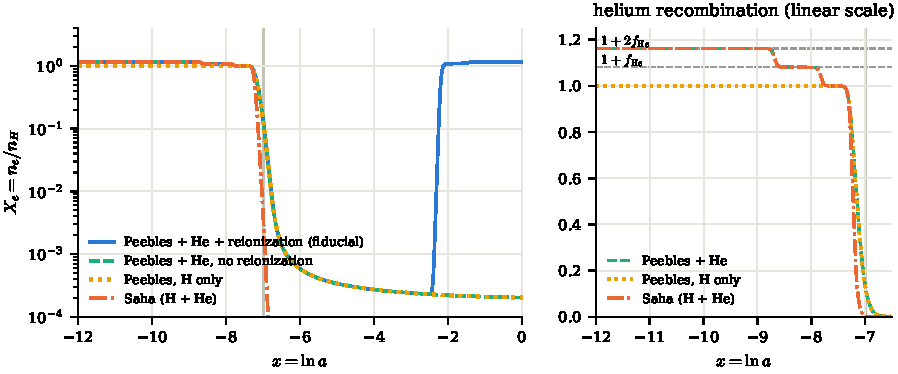
\includegraphics[width=\textwidth]{m2_Xe}
\caption{Free electron fraction. \emph{Left:} the fiducial model (Peebles hydrogen, Saha helium and reionization),
the same without reionization, the hydrogen-only Peebles solution, and the Saha solution for H and He. The vertical
line marks the last-scattering surface ($\tau=1$). \emph{Right:} the same on a linear scale, showing the two helium
recombinations at $z\approx6000$ and $z\approx2500$ before hydrogen recombination.}
\label{fig:Xe}
\end{figure*}

\paragraph*{Helium and hydrogen recombination.} Figure~\ref{fig:Xe} shows the free electron fraction. Helium
recombines first, in two steps, because its electrons are more tightly bound:
\begin{itemize}
\item He$^{++}\to$He$^+$ (54.4\,eV) at $z\approx6000$, the drop from $1.162$ to $1.081$;
\item He$^+\to$He (24.6\,eV) at $z\approx2500$, the drop from $1.081$ to $1$.
\end{itemize}
Both happen when $\chi/k_BT\approx40$, the same ``$\eta_b^{-1}$ delay'' as for hydrogen. Helium is fully neutral
long before hydrogen recombination starts. It therefore has no direct effect on the last-scattering surface; it
matters only by removing electrons at $z\gtrsim2000$, which affects the diffusion damping of small-scale anisotropies.
The hydrogen-only run gives the same numbers as the run with helium to better than $10^{-8}$ (both runs use the same
$n_H$).

Hydrogen recombines between $z\approx1500$ and $z\approx900$. With the Peebles equation $X_e=0.5$ at $z=1273$
($T=3475$\,K, $k_BT=0.30$\,eV), so indeed $\epsilon_0/k_BT\approx45$. Table~\ref{tab:m2} lists the key times. Here we
switch reionization off, so that $\tau$ measures the recombination surface alone.

\paragraph*{Saha versus Peebles.} The Saha approximation recombines far too early and too fast: $X_e=0.5$ at $z=1369$,
decoupling at $z=1291$, and $r_s$ is $11\%$ smaller. Saha assumes that the reactions are instantaneous. In reality the
$n=2$ bottleneck limits the net recombination rate: at $z=1200$ we find $C_r\approx0.007$, so most atoms that
reach $n=2$ are ionized again before they reach the ground state. Recombination therefore falls behind equilibrium.
The difference grows with time. In Saha equilibrium $X_e$ drops exponentially and reaches the numerical floor of
$10^{-30}$ in our code. In the Peebles solution the recombination rate per electron, $n_H\alpha^{(2)}X_e$, falls below
$H$ at $z\approx400$, and the residual ionization freezes at $X_e=2.0\times10^{-4}$ today. These residual electrons keep
$T_b$ coupled to $T_\gamma$ until $z\approx500$ and are important for the formation of the first molecules.

The RECFAST fudge factor 1.14 on $\alpha^{(2)}$ mimics the effect of a full multi-level atom. It speeds up recombination
slightly: $z_*$ changes by $+0.8$, $r_s$ by $0.05\%$, and the freeze-out value is lowered to $1.8\times10^{-4}$. These
small changes nevertheless matter at the precision of Planck.

\begin{table}
\caption{Recombination and decoupling without reionization for the Peebles (with Saha helium) and pure Saha
solutions. Times are cosmic times; $r_s$ is the comoving sound horizon.}
\label{tab:m2}
\begin{ruledtabular}
\begin{tabular}{lcc}
 & Peebles & Saha \\
\hline
$X_e=0.5$: $z$ & $1272.9$ & $1369.1$ \\
Recombination, $X_e=0.1$: $x$ & $-6.9696$ & $-7.1335$ \\
\phantom{Recombination,} $z$ & $1062.8$ & $1252.2$ \\
\phantom{Recombination,} $t$ [kyr] & $387.9$ & $294.1$ \\
Decoupling, $\tau=1$: $x$ & $-6.9943$ & $-7.1640$ \\
\phantom{Decoupling,} $z$ & $1089.4$ & $1291.0$ \\
\phantom{Decoupling,} $t$ [kyr] & $372.1$ & $279.2$ \\
Peak of $\gt$: $z$ & $1085.2$ & $1286.1$ \\
$r_s(\tau=1)$ [Mpc] & $144.46$ & $128.95$ \\
Drag epoch: $z_d$ & $1059.8$ & $1259.5$ \\
$r_s(z_d)$ [Mpc] & $147.08$ & $131.13$ \\
$X_e$ today & $2.03\times10^{-4}$ & $\to0$ \\
\end{tabular}
\end{ruledtabular}
\end{table}

\paragraph*{Decoupling.} The photons decouple ($\tau=1$) at $z=1090$, when the Universe is $372\,000$ years old and
$T=2970$\,K. At that moment $X_e=0.13$: decoupling does not require the gas to be fully neutral, only that the
scattering rate drops below the expansion rate. Indeed $|\tau'|=13$ at $\tau=1$, so a photon still scatters a few
more times per Hubble time, but $X_e$ is dropping so fast that these scatterings stop within $\Delta x\sim0.1$. The
comoving mean free path at that time is $16\Mpc$, compared with the horizon $\eta_*=280\Mpc$. Decoupling is at lower
$z$ than $X_e=0.5$ and higher $z$ than $X_e=0.1$ ($z=1063$). Within a few percent, ``recombination'' and ``last
scattering'' are the same event for the purpose of the CMB.

\begin{figure}
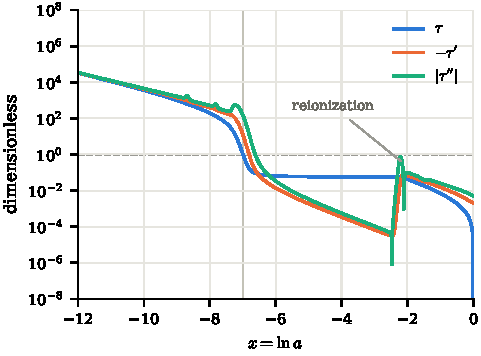
\includegraphics[width=\columnwidth]{m2_tau}
\caption{Optical depth $\tau$ and its derivatives for the fiducial model. $\tau$ drops by many orders of magnitude
during recombination. Reionization gives the shoulder at $x\approx-2$ and the total $\tau_{\rm reion}=0.058$.}
\label{fig:tau}
\end{figure}

\begin{figure*}
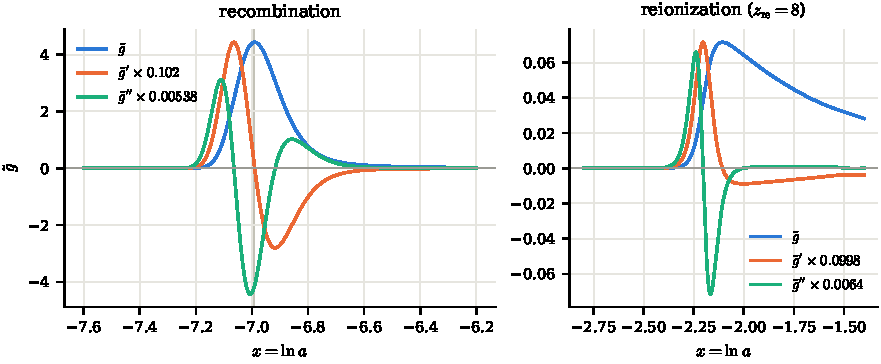
\includegraphics[width=\textwidth]{m2_g}
\caption{Visibility function $\gt$ and its first two derivatives (rescaled to the same amplitude) around recombination
(\emph{left}) and reionization (\emph{right}). The vertical line in the left panel marks $\tau=1$.}
\label{fig:g}
\end{figure*}

\paragraph*{Optical depth and visibility.} Figure~\ref{fig:tau} shows the optical depth. Before recombination
$\tau\propto$ a high power of $a^{-1}$, because $n_e\propto a^{-3}$ and $H\propto a^{-2}$ in RD. Across recombination
$|\tau'|$ drops by more than three orders of magnitude, so the Universe goes from opaque to transparent within a
small fraction of a Hubble time. Figure~\ref{fig:g} shows the visibility function. It is sharply peaked around
$x\approx-7$, with a full width at half maximum of $\Delta x\approx0.18$ ($\Delta z\approx200$). This corresponds to
a comoving thickness of $\approx39\Mpc$, about a quarter of the sound horizon. About two thirds of the CMB photons last
scattered between $z=1000$ and $z=1200$. The finite thickness of the last-scattering surface has two observable
consequences: anisotropies on scales smaller than its thickness are washed out, and polarization is generated only
within it (Sec.~\ref{sec:m3}). The derivatives $\gt'$ and $\gt''$, which appear in the source function, are smooth and
well resolved by our grid.

\paragraph*{Sound horizon and drag epoch.} At decoupling $R_b=0.62$, so the sound speed is $c_s=0.45c$, below the
relativistic value $c/\sqrt3=0.58c$. The sound horizon $r_s(z_*)=144.5\Mpc$ is therefore about half the particle
horizon. The baryons are released at the drag epoch $z_d=1060$, when the sound horizon has grown to $147.1\Mpc$. This
is the BAO scale measured in galaxy surveys.

\paragraph*{Reionization.} Reionization adds a second, broad and much lower bump in $\gt$ at $z\lesssim10$
(Fig.~\ref{fig:g}, right). The optical depth to reionization (from $z=0$ to the start of reionization,
$z_{\rm re}+8\Delta z$, as CLASS's $\tau_{\rm reio}$) is $\tau_{\rm reion}=0.0578$. For an instantaneous
reionization at $z_{\rm re}=8$ in a matter+$\Lambda$ universe,
$\tau=\int_0^{z_{\rm re}}c\sigma_Tn_e(z)\,\dd z/[(1+z)H(z)]$ gives $0.0578$ with our parameters, in agreement. This is
close to the Planck value $0.054\pm0.007$~\cite{Planck2018params}. About $1-e^{-\tau}\approx6\%$ of the CMB photons
scatter again after reionization. On scales smaller than the horizon at reionization, rescattering mixes photons from
different directions, which damps the primary anisotropies by $e^{-\tau_{\rm reion}}$ in amplitude. On larger scales it
creates new polarization: the low-$\ell$ ``reionization bump'' in $C_\ell^{EE}$ (Sec.~\ref{sec:m4}). With reionization
the electron fraction today is $X_e=1.162=1+2f_{\rm He}$.

With reionization the $\tau=1$ surface also moves slightly: $\tau_{\rm reion}$ is added to the total, so $\tau=1$ is
reached at $z_*=1084.9$ with $r_s(z_*)=144.85\Mpc$. These are the numbers to compare with CLASS, which gives
$z_*=1084.70$ and $r_s=144.87\Mpc$ (Sec.~\ref{sec:validation}).

% ===========================================================================
\section{Milestone III: Evolution of the perturbations}\label{sec:m3}
% ===========================================================================

The Universe is not perfectly homogeneous. The CMB temperature varies across the sky at the level of $10^{-5}$, and
these tiny primordial fluctuations have grown into the galaxies and clusters we see today. The third milestone follows
the fluctuations from the radiation era until today. Since they are small, we expand Einstein's equations and the
Boltzmann equations for every species to first order around the FLRW background of Milestone~I. The background is
translation invariant, so in Fourier space each wavenumber evolves independently, and isotropy means that only the
magnitude $k$ matters. The output is a set of transfer functions and source functions that the line-of-sight
integration of Milestone~IV turns into the observed spectra.

\subsection{Theory}

\paragraph*{The perturbed metric.} We work in the conformal Newtonian gauge,
\begin{equation}
\dd s^2 = a^2(\eta)\big[-(1+2\Psi)c^2\dd\eta^2 + (1+2\Phi)\delta_{ij}\dd x^i\dd x^j\big],
\end{equation}
with the variables and sign conventions of Callin~\cite{Callin2006}, which follow Dodelson~\cite{Dodelson2003}. $\Psi$
plays the role of the Newtonian gravitational potential: it governs the motion of non-relativistic particles and the
redshift of light climbing out of a potential well. $\Phi$ is a perturbation of the spatial curvature, so a changing
$\Phi$ stretches space locally and redshifts photons in the same way the background expansion does. In the absence of
anisotropic stress the two are equal and opposite, $\Psi=-\Phi$.

We write $\kappa\equiv ck/\Hp$, the wavenumber in units of the comoving Hubble scale. A mode is outside the horizon when
$\kappa\ll1$ and inside when $\kappa\gg1$; most of the interesting physics happens at horizon entry, $\kappa\approx1$.

\paragraph*{The Boltzmann equation for photons.} The photon distribution function is a Planck spectrum with a
direction-dependent temperature, $f=[\exp(p/k_BT(1+\Theta))-1]^{-1}$, where the fractional temperature perturbation
$\Theta(\bm{x},\hat{\bm p},\eta)$ depends on position and on the direction of the photon momentum. In Fourier space
$\Theta$ depends on $k$ and on $\mu=\hat{\bm k}\cdot\hat{\bm p}$. The linearized Boltzmann equation
$\dd f/\dd\eta=C[f]$ becomes
\begin{align}
\Theta' + i\kappa\mu\Theta &= -\Phi' - i\kappa\mu\Psi \nonumber\\
 &\quad - \tau'\Big[\Theta_0 - \Theta + i\mu v_b - \tfrac12P_2(\mu)\Pi\Big].
\label{eq:boltz_photon}
\end{align}
Each term has a clear physical meaning:
\begin{itemize}
\item $i\kappa\mu\Theta$ is free streaming. Photons move in direction $\hat{\bm p}$, so an inhomogeneity in space turns
      into an anisotropy in direction.
\item $-\Phi'$ is the redshift caused by the local change of spatial curvature.
\item $-i\kappa\mu\Psi$ is the gravitational redshift (or blueshift) of photons that climb out of (or fall into) a
      potential gradient.
\item The last term is Thomson scattering, at rate $-\tau'$ per unit $x$. Scattering drives the distribution towards
      isotropy, $\Theta\to\Theta_0$. Electrons moving with velocity $v_b$ Doppler shift the scattered photons, which
      gives the $\mu v_b$ term. Thomson scattering is not isotropic but goes as $1+\cos^2$ of the scattering angle, which
      gives the quadrupole term $P_2\Pi$.
\end{itemize}
We expand in Legendre polynomials,
$\Theta_\ell=\frac{1}{(-i)^\ell}\int_{-1}^1\frac{\dd\mu}{2}P_\ell(\mu)\Theta(\mu)$, and the low multipoles are the familiar
fluid quantities:
\begin{itemize}
\item the monopole $\Theta_0$ gives the density, $\delta_\gamma=4\Theta_0$ since $\rho_\gamma\propto T^4$;
\item the dipole gives the velocity, $v_\gamma=-3\Theta_1$;
\item the quadrupole $\Theta_2$ is the anisotropic stress.
\end{itemize}
Multiplying Eq.~\eqref{eq:boltz_photon} by $P_\ell$ and integrating, the $\mu\Theta$ term couples each $\ell$ to
$\ell\pm1$, because $\mu P_\ell$ is a combination of $P_{\ell-1}$ and $P_{\ell+1}$. This gives the hierarchy
\begin{align}
\Theta_0' &= -\kappa\Theta_1 - \Phi', \\
\Theta_1' &= \frac{\kappa}{3}(\Theta_0 - 2\Theta_2 + \Psi) + \tau'\Big(\Theta_1 + \frac{v_b}{3}\Big), \\
\Theta_\ell' &= \frac{\kappa\big[\ell\Theta_{\ell-1} - (\ell+1)\Theta_{\ell+1}\big]}{2\ell+1}
               + \tau'\Big(\Theta_\ell - \frac{\Pi}{10}\delta_{\ell2}\Big),
\end{align}
where the factors of $i$ have been absorbed into the definition of the velocities. The monopole equation is the
continuity equation of the photon fluid, and the dipole equation is its Euler equation. Free streaming moves power from
low to high $\ell$: an inhomogeneity on scale $1/k$ viewed from a distance $d$ appears as an anisotropy at
$\ell\sim kd$. Scattering instead damps all $\ell\ge2$ multipoles and locks $\Theta_1$ to the baryon velocity.

\paragraph*{Polarization.} Thomson scattering of radiation with a quadrupole anisotropy produces linearly polarized
light: the scattered wave is polarized perpendicular to the plane of scattering, and an incoming quadrupole makes
the polarization from different directions not cancel. Its multipoles $\Theta^P_\ell$ obey a similar
hierarchy~\cite{Zaldarriaga1995}, sourced by $\Pi=\Theta_2+\Theta^P_0+\Theta^P_2$:
\begin{align}
\Theta^{P\prime}_\ell &= \frac{\kappa\big[\ell\Theta^P_{\ell-1} - (\ell+1)\Theta^P_{\ell+1}\big]}{2\ell+1} \nonumber\\
      &\quad + \tau'\Big[\Theta^P_\ell - \frac{\Pi}{2}\Big(\delta_{\ell0}+\frac{\delta_{\ell2}}{5}\Big)\Big].
\end{align}
Polarization has no gravitational source: it is created only by scattering of a quadrupole.

\paragraph*{Neutrinos.} Neutrinos decoupled long before the earliest time we consider, so their Boltzmann equation is
Eq.~\eqref{eq:boltz_photon} without the collision term. Their multipoles $\mathcal{N}_\ell$ obey the photon hierarchy
with $\tau'=0$. Massless neutrinos therefore free-stream from the start. Their quadrupole $\mathcal{N}_2$ is a large
anisotropic stress during the radiation era, when they make up $41\%$ of the radiation density.

\paragraph*{Dark matter and baryons.} Cold dark matter is collisionless and non-relativistic. The first two moments of
its Boltzmann equation (equivalently, energy--momentum conservation) are the continuity and Euler equations,
\begin{equation}
\delta_{\rm CDM}' = \kappa v_{\rm CDM} - 3\Phi', \qquad v_{\rm CDM}' = -v_{\rm CDM} - \kappa\Psi.
\end{equation}
In the continuity equation $\kappa v$ is the inflow of matter, and $-3\Phi'$ the change of the local volume when the
spatial metric is perturbed. In the Euler equation $-v$ is the Hubble drag, which redshifts peculiar momenta as
$a^{-1}$, and $-\kappa\Psi$ is the gravitational force. Baryons obey the same equations plus the momentum they
exchange with the photons through Thomson scattering:
\begin{align}
\delta_b' &= \kappa v_b - 3\Phi', \\
v_b' &= -v_b - \kappa\Psi + \tau'R(3\Theta_1+v_b).
\end{align}
The factor $R=4\rho_\gamma/3\rho_b$ ensures momentum conservation. The momentum the photons lose (the $\tau'$ term in
the $\Theta_1$ equation) is gained by the baryons, whose momentum density is smaller by $\rho_b/(\tfrac43\rho_\gamma)$.

\paragraph*{Einstein equations.} The perturbed Einstein equations relate the potentials to the matter. The $00$
component, together with the $0i$ component, gives
\begin{align}
\Phi' &= \Psi - \frac{\kappa^2}{3}\Phi + \frac{H_0^2}{2\Hp^2}\Big[\frac{\Om_{\rm CDM}\delta_{\rm CDM}+\Om_b\delta_b}{a} \nonumber\\
      &\qquad + \frac{4(\Om_\gamma\Theta_0+\Om_\nu\mathcal{N}_0)}{a^2}\Big], \label{eq:einstein1}
\end{align}
where $\Om_i$ are today's values. Deep inside the horizon ($\kappa\gg1$) this reduces to the Poisson equation,
$k^2\Phi\propto a^2\delta\rho$. The traceless part of the $ij$ components gives
\begin{equation}
\Psi = -\Phi - \frac{12H_0^2}{c^2k^2a^2}\big[\Om_\gamma\Theta_2+\Om_\nu\mathcal{N}_2\big],
\label{eq:einstein2}
\end{equation}
so $\Psi\neq-\Phi$ only if there is anisotropic stress: the quadrupoles of the photons and neutrinos.

\paragraph*{Truncation.} We truncate the hierarchies at $\ell_{\max}$ with the closure of Ma \&
Bertschinger~\cite{Ma1995}. It assumes the free-streaming solution $\Theta_\ell\propto j_\ell(k\eta)$ for the highest
multipole, to avoid an artificial reflection of power back down to low $\ell$:
\begin{equation}
\Theta_{\ell_{\max}}' = \kappa\Theta_{\ell_{\max}-1} - \frac{c(\ell_{\max}+1)}{\Hp\eta}\Theta_{\ell_{\max}}
+\tau'\Theta_{\ell_{\max}}.
\end{equation}

\paragraph*{Initial conditions.} At $x=-18$ every mode is far outside the horizon ($\kappa\ll1$) and the Universe is
radiation dominated. Inflation produces \emph{adiabatic} fluctuations: the whole Universe is locally the same, but
slightly ahead of or behind in time. Then the number densities of all species are perturbed equally,
$\delta_{\rm CDM}=\delta_b=\tfrac34\delta_\gamma=\tfrac34\delta_\nu$. Solving the equations to lowest order in $\kappa$
gives $\Phi'=0$ and $\Theta_0=-\Psi/2$. The neutrino quadrupole in Eq.~\eqref{eq:einstein2} gives
$\Phi=-(1+2f_\nu/5)\Psi$, with $f_\nu=\Om_\nu/(\Om_\gamma+\Om_\nu)$. We normalize to a primordial comoving curvature
perturbation $\mathcal{R}=1$, which is conserved outside the horizon and is the quantity inflation predicts. Then
\begin{align}
\Psi &= -\frac{1}{\tfrac32+\tfrac25f_\nu}, \quad \Phi = -\Big(1+\frac{2f_\nu}{5}\Big)\Psi, \nonumber\\
\delta_{\rm CDM} &=\delta_b=-\frac32\Psi,\quad v_{\rm CDM} = v_b = -\frac{\kappa}{2}\Psi, \nonumber\\
\Theta_0 &=\mathcal{N}_0=-\frac{\Psi}{2},\quad \Theta_1=\mathcal{N}_1=\frac{\kappa}{6}\Psi, \nonumber\\
\mathcal{N}_2 &= -\frac{(cka)^2\Phi}{12H_0^2\Om_\nu}\Big(1+\frac{5}{2f_\nu}\Big)^{-1},
\end{align}
and $\mathcal{N}_\ell=\kappa\mathcal{N}_{\ell-1}/(2\ell+1)$ for $\ell\ge3$. The actual amplitude of each mode is
restored in Milestone~IV through the primordial power spectrum $\mathcal{P}_{\mathcal{R}}(k)$.

\paragraph*{Tight coupling and acoustic oscillations.} At early times $|\tau'|\gg1$: a photon scatters thousands of
times per Hubble time. The scattering terms force $\Theta_1\simeq-v_b/3$, and the photon multipoles with $\ell\ge2$ are
suppressed by powers of $\kappa/\tau'$. The photons and baryons then behave as one fluid. Combining the $\Theta_0$,
$\Theta_1$ and $v_b$ equations at leading order in $1/\tau'$ gives, in conformal time,
\begin{align}
\frac{\dd}{\dd\eta}\Big[(1+R_b)\dot\Theta_0\Big] + \frac{c^2k^2}{3}\Theta_0
 &= -\frac{c^2k^2}{3}(1+R_b)\Psi \nonumber\\
 &\quad - \frac{\dd}{\dd\eta}\Big[(1+R_b)\dot\Phi\Big],
\label{eq:oscillator}
\end{align}
with $R_b=1/R=3\rho_b/4\rho_\gamma$. This is a driven harmonic oscillator. Photon pressure provides the restoring force,
baryons add inertia ($1+R_b$) and lower the sound speed to $c_s=c/\sqrt{3(1+R_b)}$, and gravity drives it. For slowly
varying potentials and $R_b$ the adiabatic solution is
\begin{equation}
\Theta_0+(1+R_b)\Psi \simeq A\cos(kr_s),
\label{eq:acoustic}
\end{equation}
where $r_s$ is the sound horizon of Milestone~II. These are the acoustic oscillations of the photon--baryon fluid. Two
features are important for the CMB:
\begin{itemize}
\item The observed temperature includes the gravitational redshift, $\Theta_0+\Psi=A\cos(kr_s)-R_b\Psi$. Baryons shift
      the zero point of the oscillation, so compressions in potential wells are enhanced relative to rarefactions.
\item When a mode enters the horizon in RD, the potentials decay just as the fluid is first compressed. The decay
      removes the gravitational pull that would otherwise slow the rebound, which boosts the oscillation amplitude
      (``radiation driving'').
\end{itemize}

At next order in $1/\tau'$ photons diffuse over their mean free path and smooth out the oscillations (Silk damping):
$\Theta_0\propto e^{-k^2/k_D^2}$ with~\cite{HuSugiyama1995}
\begin{equation}
k_D^{-2} = \int_0^\eta \frac{c\,\dd\eta'}{6(1+R_b)\,n_e\sigma_Ta}\Big[\frac{R_b^2}{1+R_b}+\frac{16}{15}\Big].
\label{eq:silk}
\end{equation}
This is a random walk: the diffusion length is the geometric mean of the mean free path and the horizon.

Numerically, the tight-coupling regime is too stiff to integrate the full hierarchy. We evolve only
$\delta_{\rm CDM},v_{\rm CDM},\delta_b,v_b,\Phi,\Theta_0,\Theta_1$ (and the neutrinos), and set
\begin{equation}
\Theta_2 = -\frac{8}{15}\frac{\kappa}{\tau'}\Theta_1, \quad \Theta^P_0=\frac54\Theta_2, \quad \Theta^P_2=\frac14\Theta_2,
\end{equation}
with $\Theta_\ell=-\frac{\ell}{2\ell+1}\frac{\kappa}{\tau'}\Theta_{\ell-1}$ for $\ell\ge3$ (and the same for
$\Theta^P$). These are the quasi-static solutions of the hierarchy when the $\tau'$ terms dominate. Without polarization,
$8/15$ becomes $20/45$. Polarization feeds back on $\Theta_2$ through $\Pi$, which raises the quadrupole by a factor
$6/5$. The baryon velocity and $\Theta_1$ follow from the second-order expansion of Ref.~\cite{Callin2006}, which
eliminates the large $\tau'$ terms in favour of the slip $q\equiv3\Theta_1'+v_b'$:
\begin{align}
q &= \Big\{-[(1-R)\tau'+(1+R)\tau'']\,(3\Theta_1+v_b) - \kappa\Psi \nonumber\\
  &\qquad + \Big(1-\frac{\Hp'}{\Hp}\Big)\kappa(-\Theta_0+2\Theta_2) - \kappa\Theta_0'\Big\} \nonumber\\
  &\quad \Big/\Big[(1+R)\tau'+\frac{\Hp'}{\Hp}-1\Big], \nonumber\\
v_b' &= \frac{-v_b - \kappa\Psi + R\big[q + \kappa(-\Theta_0+2\Theta_2) - \kappa\Psi\big]}{1+R}, \nonumber\\
\Theta_1' &= \frac{1}{3}(q - v_b').
\end{align}
Tight coupling ends when $|\tau'|<10$, when $|\kappa/\tau'|>0.1$, or at $z=1700$ (before recombination starts),
whichever comes first.

\paragraph*{Analytic limits.} A few exact results guide the interpretation and serve as tests:
\begin{itemize}
\item Outside the horizon $\Phi$ is constant within each era. Through radiation--matter equality it drops by the factor
      $9/10$ (without neutrinos). With $\mathcal{R}=1$, $\Phi=3/5$ in MD. The full superhorizon solution through
      equality is known analytically~\cite{Kodama1984}.
\item Inside the horizon in RD, the potential obeys $\Phi=3\Phi_0(\sin y-y\cos y)/y^3$ with $y=k\eta/\sqrt3$. It
      oscillates and decays as $a^{-2}$, because radiation pressure prevents the density contrast from growing while
      the background density falls as $a^{-4}$.
\item In MD $\Phi$ is constant on all scales: $\delta\propto a$ and $\rho_Ma^2\propto a^{-1}$ cancel in the Poisson
      equation. In the $\Lambda$ era $\Phi\propto D(a)/a$ decays, where $D$ is the linear growth factor.
\item Sub-horizon dark matter obeys $\ddot\delta+2H\dot\delta=4\pi G\rho_M\delta$ (ignoring the radiation
      perturbations). In RD the source is negligible and $\delta\propto\ln a$ (the M\'esz\'aros effect). In MD
      $\delta\propto a$. In general the growth rate is $f=\dd\ln\delta/\dd\ln a\approx\Om_M(x)^{0.55}$.
\end{itemize}

\paragraph*{Source functions.} After the evolution we build the temperature and $E$-mode source functions:
\begin{align}
S_T(k,x) &= \gt\Big[\Theta_0+\Psi+\frac{\Pi}{4}\Big] + e^{-\tau}(\Psi'-\Phi') \nonumber\\
 &\quad - \frac{1}{ck}\frac{\dd}{\dd x}(\Hp\gt v_b)
  + \frac{3}{4c^2k^2}\frac{\dd}{\dd x}\Big[\Hp\frac{\dd}{\dd x}(\Hp\gt\Pi)\Big], \label{eq:ST}\\
S_E(k,x) &= \frac{3\gt\,\Pi}{4k^2(\eta_0-\eta)^2}. \label{eq:SE}
\end{align}
They come from integrating Eq.~\eqref{eq:boltz_photon} along the line of sight (Sec.~\ref{sec:m4}); the derivatives
arise from integrating the $\mu$-dependent terms by parts. They express the temperature we see as a sum over all
places where a photon last scattered (weighted by $\gt$) or was redshifted on its way (weighted by $e^{-\tau}$). The
four terms are, in order:
\begin{itemize}
\item the Sachs--Wolfe (SW) term: the intrinsic temperature at last scattering plus the gravitational redshift out of
      the potential well there;
\item the integrated Sachs--Wolfe (ISW) term: the net energy change of a photon crossing a time-varying potential;
\item the Doppler term: from the velocity of the electrons that last scattered the photon;
\item a small correction from the anisotropic, polarization-dependent nature of Thomson scattering.
\end{itemize}

\subsection{Implementation and tests}

\texttt{Perturbations} solves 400 modes, logarithmically spaced in $k\in[5\times10^{-5},0.3]\Mpc^{-1}$, on a
non-uniform grid of 2100 points in $x\in[-18,0]$ that is dense around recombination. The modes run in parallel with
OpenMP. We keep $\ell_{\max}=8$ for $\Theta_\ell$ and $\Theta^P_\ell$, and $\ell_{\max,\nu}=22$ for the neutrinos;
going to $\ell_{\max,\nu}=30$ changes the spectra by less than $5\times10^{-4}$. Only the low photon multipoles enter
the sources, so a small $\ell_{\max}$ is enough. The tight-coupling system is solved with an explicit Runge--Kutta
method (RK8PD). The full system is stiff, because $|\tau'|$ is still large when tight coupling ends, so we use the
implicit BDF method of GSL with a finite-difference Jacobian. The relative tolerance is $10^{-8}$. At the switch we
initialize the full hierarchy from the tight-coupling expressions above. The derivatives in $S_T$ come from splines in
$x$, and all quantities are stored as 2D bicubic splines in $(x,k)$.

The tests (Fig.~\ref{fig:m3_tests} and the unit tests) check the analytic limits listed above:
\begin{itemize}
\item On superhorizon scales the solution matches the exact Kodama--Sasaki solution through equality, and
      $\Phi\to3/5$ in MD.
\item For modes that enter in RD, $\Phi$ follows the analytic radiation-era solution until equality approaches
      (middle panel).
\item Before decoupling, $\Theta_0+\Psi$ oscillates as $\cos(kr_s)$, with the phase given by the sound horizon of
      Milestone~II (left panel). This tests the sound speed, and with it $R$.
\item In matter and $\Lambda$ domination the growth rate $\dd\ln\delta_{\rm CDM}/\dd x$ of small-scale modes follows
      $\Om_M(x)^{0.55}$ (right panel).
\end{itemize}
In addition, the Poisson equation holds on subhorizon scales today, the tight-coupling and full solutions are
continuous at the switch, and the neutrino multipoles free-stream as expected. All perturbations agree with CLASS to
$\sim0.1\%$.

\begin{figure*}
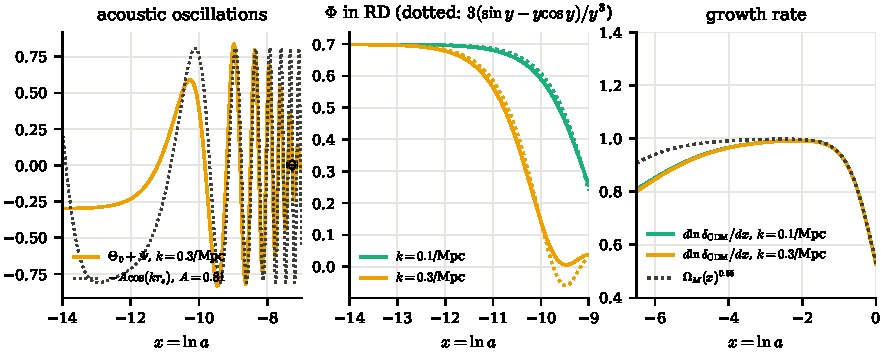
\includegraphics[width=\textwidth]{m3_tests}
\caption{Tests of the perturbations. \emph{Left:} $\Theta_0+\Psi$ for $k=0.3\Mpc^{-1}$ during the radiation era
compared with $-A\cos(kr_s)$, using the sound horizon $r_s$ from Milestone~II. After horizon entry the decaying
potential drives the oscillator, so the amplitude $A$ is fitted; the test is the phase. \emph{Middle:} $\Phi$ for
modes that enter in RD, compared with the analytic radiation-era solution (dotted). \emph{Right:} the growth rate of
$\delta_{\rm CDM}$ compared with $\Om_M(x)^{0.55}$.}
\label{fig:m3_tests}
\end{figure*}

\subsection{Results}

We show four modes, chosen to probe the different regimes:
\begin{itemize}
\item $k=0.001\Mpc^{-1}$ enters the horizon ($\kappa=1$) at $x=-4.13$ ($z\approx61$), well into MD. It is
      outside the horizon at recombination and probes the largest scales in the CMB.
\item $k=0.01\Mpc^{-1}$ enters at $x=-8.08$, close to equality.
\item $k=0.1\Mpc^{-1}$ enters at $x=-10.71$ and $k=0.3\Mpc^{-1}$ at $x=-11.83$, both deep in RD. They oscillate many
      times before recombination.
\end{itemize}
Tight coupling ends at $x=-7.44$ ($z=1700$) for the first three modes, and at $x=-7.89$ for $k=0.3\Mpc^{-1}$, where
$\kappa/\tau'$ becomes large first. Horizon entry is marked by coloured dotted lines in the figures, and grey lines mark
radiation--matter equality and decoupling.

\begin{figure*}
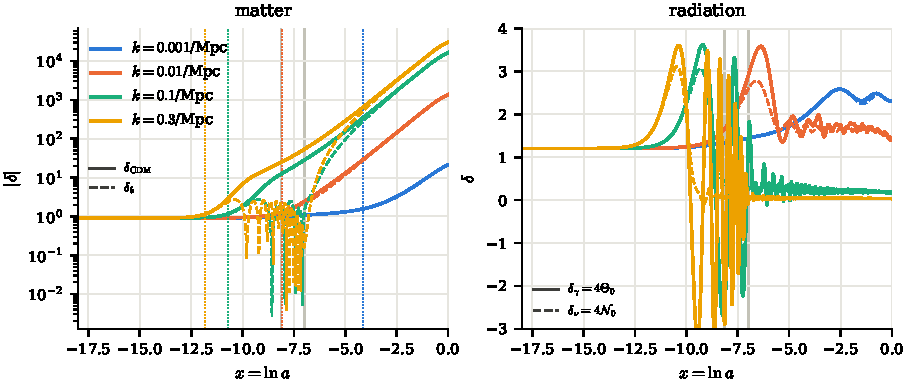
\includegraphics[width=\textwidth]{m3_delta}
\caption{Density perturbations. \emph{Left:} $|\delta_{\rm CDM}|$ (solid) and $|\delta_b|$ (dashed). The coloured
dotted lines mark horizon entry of each mode. \emph{Right:} photon $\delta_\gamma=4\Theta_0$ (solid) and neutrino
$\delta_\nu=4\mathcal{N}_0$ (dashed). Grey lines mark radiation--matter equality and decoupling ($\tau=1$).}
\label{fig:delta}
\end{figure*}

\begin{figure*}
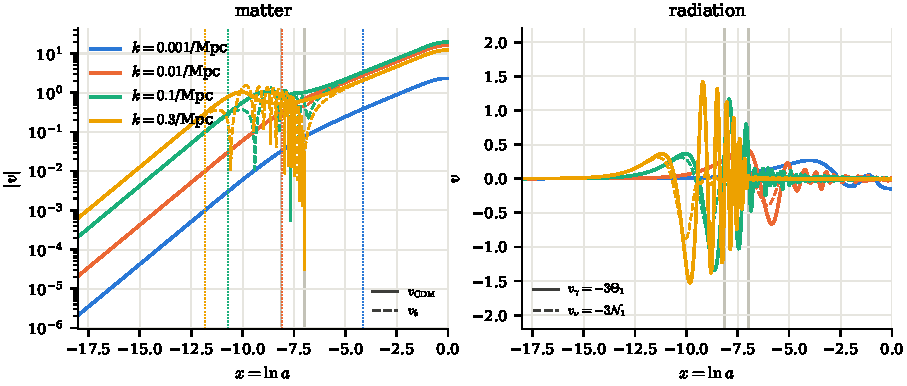
\includegraphics[width=\textwidth]{m3_velocity}
\caption{Velocities. \emph{Left:} $|v_{\rm CDM}|$ (solid) and $|v_b|$ (dashed). \emph{Right:} photon
$v_\gamma=-3\Theta_1$ (solid) and neutrino $v_\nu=-3\mathcal{N}_1$ (dashed).}
\label{fig:velocity}
\end{figure*}

\paragraph*{Dark matter.} Figure~\ref{fig:delta} shows the density contrasts. Outside the horizon all $\delta$'s are
nearly constant at $\delta=-\frac32\Psi$. There is no causal mechanism to change them, and in our gauge the
superhorizon density contrast only changes through the changing potential at equality. After horizon entry the
behaviour of $\delta_{\rm CDM}$ depends on when the mode entered:
\begin{itemize}
\item Modes that enter in RD ($k=0.1$, $0.3\Mpc^{-1}$) receive a kick from the decaying potential at horizon entry.
      After that they grow only slowly, because the dark matter's self-gravity is negligible compared with the
      expansion driven by the smooth radiation. The dark matter coasts on the velocity it got at entry, and
      $\delta_{\rm CDM}$ grows logarithmically (the M\'esz\'aros effect).
\item After equality, matter dominates gravity and all modes grow as $\delta_{\rm CDM}\propto a$.
\item In the $\Lambda$ era growth slows down (Fig.~\ref{fig:m3_tests}, right). For $k=0.1\Mpc^{-1}$, $\delta_{\rm CDM}$
      grows by a factor 107 from $x=-5$ to today, instead of $e^5=148$ for $\delta\propto a$.
\item The mode $k=0.001\Mpc^{-1}$ starts to grow as it approaches horizon entry in MD and has not reached the
      $\delta\propto a$ regime until late.
\end{itemize}
Small scales enter earlier and spend more time inside the horizon, but the time they spend in RD is lost to the
M\'esz\'aros stagnation. This suppression of modes with $k>k_{\rm eq}$ is the origin of the turnover in $P(k)$
(Sec.~\ref{sec:m4}).

\paragraph*{Baryons.} As long as they are tightly coupled to the photons, the baryons share the photon acoustic
oscillations, and adiabaticity gives $\delta_b\simeq\frac34\delta_\gamma$. Their density contrast is stuck at the photon
level, while $\delta_{\rm CDM}$ already grows. After decoupling the baryons lose the photon pressure and fall into the
potential wells that the dark matter has built. In MD the solution is $\delta_b\simeq\delta_{\rm CDM}(1-a_d/a)$, so
within a few $e$-folds $\delta_b$ catches up. For $k=0.1\Mpc^{-1}$, $\delta_b/\delta_{\rm CDM}$ goes from $0.04$ at
$x=-7$ to $0.29$ at $x=-6$ and $0.93$ at $x=-3$; today they are equal to within $0.5\%$. The remaining difference is the
acoustic imprint, the BAO. Without dark matter the baryon perturbations would have had to grow from their value at
decoupling, $\delta_b\sim10^{-5}\times$ (a few), by only the factor $\sim10^3$ available since recombination. That is
not enough to form galaxies. Dark matter is needed to give structure a head start.

\paragraph*{Photons and neutrinos.} The photons (Fig.~\ref{fig:delta}, right) oscillate after horizon entry: these
are the acoustic oscillations of Eq.~\eqref{eq:acoustic}. The amplitude grows at horizon entry because of radiation
driving, and the oscillation is offset from zero by the baryon loading term $-R_b\Psi$. Diffusion then damps the
oscillation. At decoupling $k_D\approx0.14\Mpc^{-1}$ (Eq.~\ref{eq:silk}), so the $k=0.3\Mpc^{-1}$ mode has lost most
of its amplitude: $|\Theta_0+\Psi|$ drops from $0.84$ at $x\approx-9$ to $0.2$ at decoupling. The $k=0.1\Mpc^{-1}$ mode
is only mildly damped. After decoupling the photons free-stream, $\Theta_0$ decays, and the power moves to higher
multipoles; at late times $\Theta_0\approx-\Psi$, so that the observed
$\Theta_0+\Psi$ averages to zero inside the horizon.

The neutrinos have been free-streaming all along. They have no pressure that can restore an acoustic oscillation, so
$\delta_\nu$ oscillates with decaying amplitude like a Bessel function as soon as the mode enters the horizon.

\paragraph*{Velocities.} The velocities (Fig.~\ref{fig:velocity}) tell the same story. Outside the horizon
$v\propto\kappa$ grows as the mode approaches the horizon. In MD the continuity equation gives $v=\delta'/\kappa
\propto a/a^{1/2}=a^{1/2}$: $v_{\rm CDM}$ grows by a factor 2.65 between $x=-3$ and $x=-1$ for $k=0.1\Mpc^{-1}$, close to
$e^{1}=2.72$. Growth slows in the $\Lambda$ era. $v_b$ oscillates with the photons until decoupling (as $\Theta_1$, out
of phase with $\Theta_0$) and then quickly joins $v_{\rm CDM}$. The photon velocity $-3\Theta_1$ oscillates in
quadrature with the density, which is the origin of the Doppler term in the CMB.

\begin{figure}
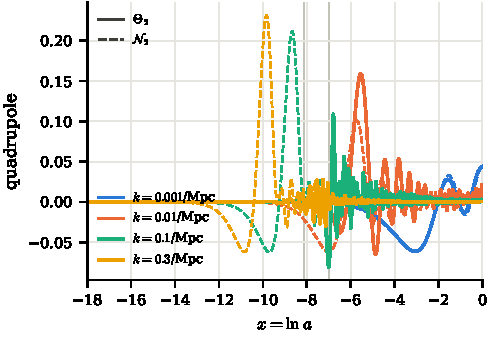
\includegraphics[width=\columnwidth]{m3_quadrupole}
\caption{Photon quadrupole $\Theta_2$ (solid) and neutrino quadrupole $\mathcal{N}_2$ (dashed).}
\label{fig:quadrupole}
\end{figure}

\begin{figure}
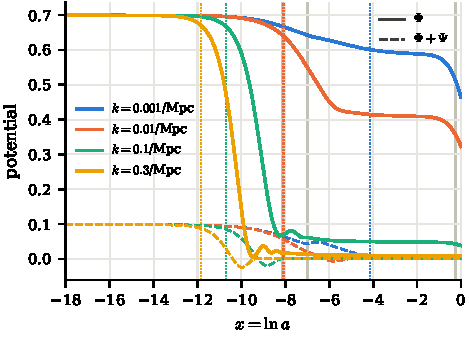
\includegraphics[width=\columnwidth]{m3_Phi}
\caption{Potentials $\Phi$ (solid) and $\Phi+\Psi$ (dashed). $\Phi+\Psi\neq0$ is the anisotropic stress of the
neutrinos, which is significant only during RD.}
\label{fig:Phi}
\end{figure}

\paragraph*{Quadrupoles.} The photon quadrupole (Fig.~\ref{fig:quadrupole}) is suppressed by scattering until
recombination, $\Theta_2\propto(\kappa/\tau')\Theta_1$: every scattering erases the anisotropy. As $|\tau'|$ falls
during recombination it grows rapidly, and after decoupling it reaches about a quarter of $\Theta_0$ as the photons
free-stream. The neutrino quadrupole is present from the start, since nothing isotropizes the neutrinos.

\paragraph*{Potentials.} Figure~\ref{fig:Phi} shows the potentials.
\begin{itemize}
\item $\Phi$ is constant outside the horizon. The neutrino anisotropic stress makes $\Phi+\Psi\neq0$: in RD
      $\Phi/\Psi=-(1+2f_\nu/5)$, a $16\%$ effect. As matter takes over, the neutrinos' share of the energy, and with it
      $\Phi+\Psi$, falls; it also decays once a mode is inside the horizon and the neutrinos have dispersed.
\item For modes that enter in RD, $\Phi$ decays and oscillates after horizon entry, as in the analytic solution.
      Radiation pressure keeps the photon density perturbation from growing while the background radiation density
      falls as $a^{-4}$, so the potential it sources decays as $a^{-2}$.
\item Once matter dominates, $\Phi$ is constant on all scales: the growing matter perturbation exactly compensates the
      dilution of the background. This is why $\Phi$ for $k=0.1$ and $0.3\Mpc^{-1}$ freezes at a small value after
      equality.
\item For $k=0.001\Mpc^{-1}$ we see the superhorizon transition from $0.699$ in RD to $0.586$ at $x=-1.5$, close to the
      MD value $3/5$; the ratio $0.84$ differs from $9/10$ because of the neutrinos.
\item When $\Lambda$ takes over, growth slows down and all potentials decay, by about $20\%$ today. This late decay is
      the source of the late ISW effect in the CMB.
\end{itemize}

\begin{figure*}
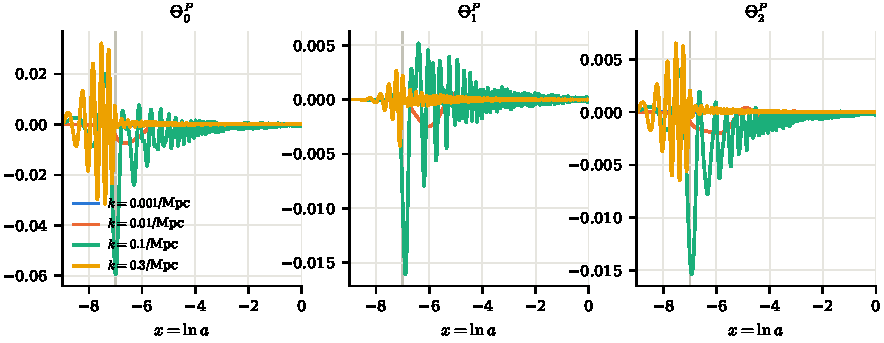
\includegraphics[width=\textwidth]{m3_polarization}
\caption{Polarization multipoles $\Theta^P_0$, $\Theta^P_1$ and $\Theta^P_2$ from shortly before decoupling (grey
line) until today.}
\label{fig:polarization}
\end{figure*}

\paragraph*{Polarization.} The polarization multipoles (Fig.~\ref{fig:polarization}) are generated only by Thomson
scattering of a quadrupole. Polarization therefore needs two things at once: scattering, and a quadrupole. Before
recombination the scattering is so efficient that the quadrupole is tiny, $\Theta_2\sim(\kappa/\tau')\Theta_1$. After
decoupling the quadrupole is large, but there is no more scattering. Polarization is produced only during the short
interval when the photons are starting to free-stream but still scattering occasionally, i.e.\ during the width of the
visibility function. Since $\Theta_2\propto\kappa\Theta_1$, the polarization traces the photon \emph{velocity}, not the
density, at last scattering. As a result:
\begin{itemize}
\item the $E$-mode signal is about a factor 10 weaker than the temperature signal;
\item it is very sensitive to the duration of recombination;
\item its acoustic peaks are out of phase with those of the temperature (Sec.~\ref{sec:m4}).
\end{itemize}
After decoupling the multipoles free-stream and decay. Reionization gives a small second burst at $x\approx-2$,
which is responsible for the low-$\ell$ $E$-mode bump.

% ===========================================================================
\section{Milestone IV: The CMB and matter power spectra}\label{sec:m4}
% ===========================================================================

The last milestone turns the source functions of Milestone~III into observables: the angular power spectra of the
CMB temperature and polarization, and the matter power spectrum today. We also interpret the shapes of these spectra
in terms of the physics of the earlier milestones.

\subsection{Theory}

\paragraph*{Statistics of the CMB sky.} The temperature fluctuation in direction $\hat{\bm n}$ is expanded in
spherical harmonics, $\Theta(\hat{\bm n})=\sum_{\ell m}a_{\ell m}Y_{\ell m}(\hat{\bm n})$. Multipole $\ell$ corresponds
to an angular scale $\theta\approx\pi/\ell$. The primordial fluctuations are a statistically homogeneous and
isotropic random field, so the $a_{\ell m}$ are uncorrelated and their variance depends only on $\ell$:
$\langle a_{\ell m}a^*_{\ell'm'}\rangle=\delta_{\ell\ell'}\delta_{mm'}C_\ell$. All the information in a Gaussian field is
in the power spectrum $C_\ell$. Since only $2\ell+1$ values of $m$ are available for each $\ell$, $C_\ell$ can only be
measured with a relative precision of $\sqrt{2/(2\ell+1)}$ (cosmic variance), which dominates the error bars at
low $\ell$.

The primordial curvature perturbation has the power spectrum
$\langle\mathcal{R}(\bm k)\mathcal{R}^*(\bm k')\rangle=(2\pi)^3\delta^3(\bm k-\bm k')\,2\pi^2\mathcal{P}_{\mathcal{R}}(k)/k^3$,
with $\mathcal{P}_{\mathcal{R}}=A_s(k/k_{\rm pivot})^{n_s-1}$. Inflation predicts a nearly scale-invariant spectrum,
$n_s\simeq1$, in which every logarithmic interval of $k$ contributes equally to the curvature fluctuations. Because the
evolution is linear and every mode in Milestone~III was normalized to $\mathcal{R}=1$, every observable is a
primordial amplitude times a transfer function.

\paragraph*{The line-of-sight integral.} A direct solution of the photon hierarchy up to $\ell\sim2500$ would need
thousands of coupled equations per mode. Seljak and Zaldarriaga~\cite{Seljak1996} noticed that Eq.~\eqref{eq:boltz_photon}
is a linear first-order equation in $\Theta$ that can be integrated formally. In conformal time it has the form
$\dot\Theta+(ik\mu-\dot\tau)\Theta=\tilde S$, where $\tilde S$ collects all terms that do not contain $\Theta$
itself. With the integrating factor $e^{ik\mu\eta-\tau}$ and $\tau(\eta_0)=0$,
\begin{equation}
\Theta(k,\mu,\eta_0)=\int_0^{\eta_0}\tilde S(k,\mu,\eta)\,e^{-\tau(\eta)}\,e^{-ik\mu(\eta_0-\eta)}\,\dd\eta .
\end{equation}
The temperature today is a sum of contributions emitted along the photon path, each attenuated by the probability
$e^{-\tau}$ that the photon is not scattered again. The phase factor is a plane wave, which the Rayleigh formula
$e^{-ik\mu\chi}=\sum_\ell(-i)^\ell(2\ell+1)j_\ell(k\chi)P_\ell(\mu)$ expands into spherical Bessel functions. After
integrating the $\mu$-dependent terms of the source by parts we obtain
\begin{align}
\Theta_\ell(k) &= \int_{-\infty}^{0} S_T(k,x)\,j_\ell[k(\eta_0-\eta)]\,\dd x, \label{eq:los}\\
\Theta^E_\ell(k) &= \sqrt{\frac{(\ell+2)!}{(\ell-2)!}}\int_{-\infty}^{0} S_E(k,x)\,j_\ell[k(\eta_0-\eta)]\,\dd x,
\end{align}
with the source functions of Eqs.~\eqref{eq:ST} and \eqref{eq:SE}. This separates the problem into physics
(the source $S$, which only needs the low multipoles and is smooth in $k$) and geometry (the Bessel function, which
projects a plane wave at distance $\eta_0-\eta$ onto multipole $\ell$). The function $j_\ell(z)$ peaks near $z\approx\ell$,
so a perturbation of wavenumber $k$ on the last-scattering surface at distance $\chi_*=\eta_0-\eta_*$ is seen mainly at
$\ell\approx k\chi_*$. The angular power spectra are
\begin{equation}
C_\ell^{XY} = 4\pi\int_0^\infty\frac{\dd k}{k}\,\mathcal{P}_{\mathcal{R}}(k)\,\Theta^X_\ell(k)\,\Theta^Y_\ell(k),
\label{eq:cl}
\end{equation}
with $X,Y\in\{T,E\}$. We plot $D_\ell=\ell(\ell+1)C_\ell/2\pi$ in $\mu$K$^2$, multiplying by $(10^6T_{\rm CMB})^2$;
$D_\ell$ is the variance of the temperature per logarithmic interval in $\ell$.

\paragraph*{The Sachs--Wolfe plateau.} On scales larger than the sound horizon at decoupling the photons have not
oscillated, and only the SW term contributes, $\Theta_\ell\approx(\Theta_0+\Psi)(k,\eta_*)\,j_\ell(k\chi_*)$. In MD the
adiabatic initial conditions give $\Theta_0=-\tfrac23\Psi$, so the observed temperature is $\Theta_0+\Psi=\Psi/3$: the
photons from a potential well start out hotter, but lose more energy climbing out. With $\Psi=-\tfrac35\mathcal{R}$,
$\Theta_0+\Psi=-\mathcal{R}/5$. Using $\int_0^\infty j_\ell^2(z)\,\dd z/z=1/[2\ell(\ell+1)]$ we find, for $n_s=1$,
\begin{equation}
D_\ell^{\rm SW} = \frac{A_s}{25}T_{\rm CMB}^2 \approx 620\muK,
\label{eq:SWplateau}
\end{equation}
independent of $\ell$. A scale-invariant primordial spectrum gives a flat $D_\ell$ on large scales.

\paragraph*{Acoustic peaks.} On smaller scales the SW term is the acoustic oscillation of Eq.~\eqref{eq:acoustic},
frozen at decoupling, $\Theta_0+\Psi\propto\cos(kr_{s*})$. Modes that are at an extremum at decoupling,
$k_nr_{s*}=n\pi$, give peaks in the spectrum. They project to
\begin{equation}
\ell_n\approx n\,\ell_A - \phi_n,\qquad \ell_A=\frac{\pi\chi_*}{r_{s*}},
\label{eq:lA}
\end{equation}
where $\phi_n$ is a phase shift caused by the driving potentials and by the projection. Odd peaks ($n=1,3,\dots$) are
compressions in potential wells and even peaks are rarefactions. The Doppler term $\propto v_b\propto\sin(kr_s)$ is
out of phase with the density and fills in the troughs between the peaks. On small scales diffusion damping suppresses
the power by $\sim e^{-2(\ell/\ell_D)^2}$, with $\ell_D=k_D\chi_*$.

\paragraph*{The matter power spectrum.} The matter power spectrum follows from $\Phi$ through the Poisson equation.
We use the comoving-gauge density contrast, which is the gauge-invariant quantity that reduces to the Newtonian density
contrast inside the horizon (in the code we evaluate it directly as
$\sum_i\rho_i[\delta_i-3\Hp v_i/(ck)]/\sum_i\rho_i$ for CDM and baryons, which is the same up to radiation terms of
order $10^{-3}$ on the largest scales; Sec.~\ref{sec:neutrinos}),
\begin{equation}
\Delta_M(k,x) = \frac{2}{3}\frac{c^2k^2}{\Hp^2}\frac{\Phi(k,x)}{\Om_M(x)},
\label{eq:DeltaM}
\end{equation}
and $P(k,x)=|\Delta_M(k,x)|^2\,2\pi^2\mathcal{P}_{\mathcal{R}}(k)/k^3$. Its shape follows from Milestone~III:
\begin{itemize}
\item For $k\ll k_{\rm eq}$ the mode entered during MD, $\Phi$ is constant and the same for all such $k$. Then
      $\Delta_M\propto k^2$ and $P\propto k^4\mathcal{P}_{\mathcal{R}}/k^3\propto k^{n_s}$.
\item For $k\gg k_{\rm eq}$ the potential decayed in RD by $\sim(k_{\rm eq}/k)^2$, partly compensated by the
      logarithmic M\'esz\'aros growth. This gives $P\propto k^{n_s-4}\ln^2(k/k_{\rm eq})$.
\end{itemize}
The spectrum therefore peaks near $k_{\rm eq}$. Because $k_{\rm eq}\propto\Om_{M0}h^2$ in units of Mpc$^{-1}$, the
peak position measures the matter density.

\subsection{Implementation and tests}

\texttt{PowerSpectrum} first tabulates $j_\ell(z)$ for all needed $\ell$ on a uniform grid with 32 points per
$2\pi$, and $j_\ell(z)/z^2$ for the $E$-mode source of Eq.~\eqref{eq:SE}. Uniform grids allow $O(1)$ spline lookups.
We evaluate Eq.~\eqref{eq:los} by the trapezoidal rule on an $x$-grid that starts at $x=-8.5$, when $e^{-\tau}$ makes
the source negligible. The grid has spacing $\Delta x=0.003$ around recombination, to resolve $\gt$, and is uniform in
$\eta$ elsewhere, with five points per Bessel oscillation at $k_{\max}$. The $k$-integral uses four points per period
$2\pi/\eta_0$ of the transfer functions (and $\Delta\ln k\le0.02$ at small $k$), up to $k_{\max}=0.3\Mpc^{-1}$, i.e.\
$k\eta_0\approx4300$. We compute $C_\ell$ at 97 multipoles between 2 and 2500 and spline in $\ell$. The full run
(background, recombination, perturbations and spectra) takes about 60\,s on two cores.

Tests include:
\begin{itemize}
\item The SW term alone gives the plateau of Eq.~\eqref{eq:SWplateau} at low $\ell$, corrected for the effects
      discussed below.
\item The peak spacing agrees with $\ell_A$ from the sound horizon and $\chi_*$.
\item $C_\ell^{EE}\ge0$ and $|C_\ell^{TE}|\le\sqrt{C_\ell^{TT}C_\ell^{EE}}$.
\item Doubling the LOS and $k$ sampling changes the spectra by less than $5\times10^{-5}$.
\item $P(k)$ has slope $n_s$ at small $k$ and turns over at $k_{\rm eq}$.
\end{itemize}

\subsection{Results}

\begin{figure}
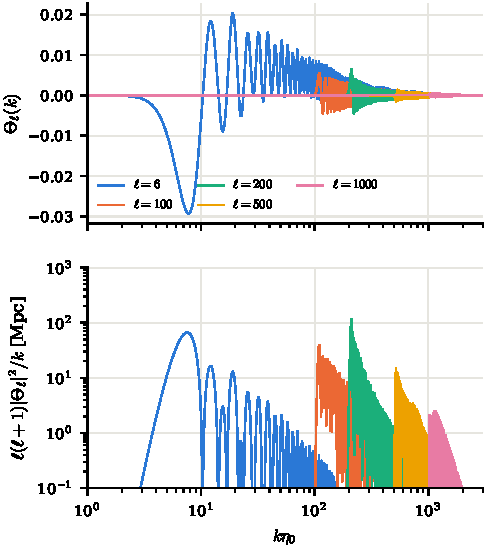
\includegraphics[width=\columnwidth]{m4_transfer}
\caption{Photon transfer functions $\Theta_\ell(k)$ (\emph{top}) and the integrand $\ell(\ell+1)\Theta_\ell^2/k$ of
$C_\ell$ (\emph{bottom}) for $\ell=6$, 100, 200, 500 and 1000, as functions of $k\eta_0$.}
\label{fig:transfer}
\end{figure}

\paragraph*{Transfer functions.} Figure~\ref{fig:transfer} shows the projection at work. $\Theta_\ell(k)$ is zero for
$k\eta_0<\ell$, where $j_\ell$ vanishes: a wave cannot produce structure on angles smaller than its own projected
wavelength. It peaks at $k\eta_0\simeq\ell$ (more precisely $k\chi_*\simeq\ell$), where the wave vector is
perpendicular to the line of sight. It then oscillates with a slowly decaying tail from waves whose wave vector is
inclined to the line of sight; their crests are farther apart on the sky, so they project onto larger angles. Each
multipole therefore receives contributions from a range of $k$, which smears the acoustic features: the peaks in $C_\ell$
are much broader than the oscillations of $\Theta_0(k)$ at recombination. The integrand of $C_\ell$ (bottom panel) is
dominated by the first peak at $k\chi_*\approx\ell$. Its height follows the acoustic oscillations: $\ell=200$ sits on
the first peak and has a much larger integrand than $\ell=100$, while $\ell=1000$ is suppressed by damping.

\begin{figure}
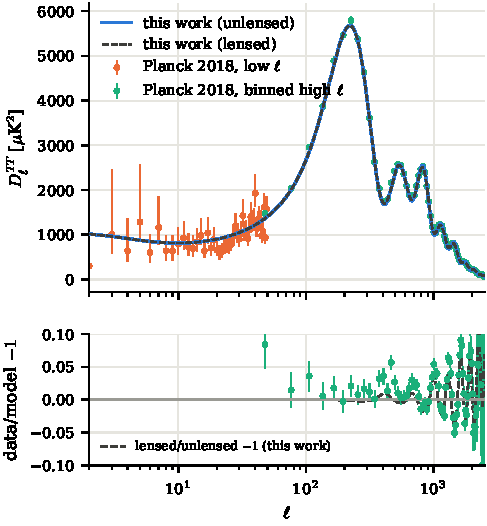
\includegraphics[width=\columnwidth]{m4_TT_planck}
\caption{\emph{Top:} our TT spectrum, unlensed and lensed, compared with Planck 2018 data~\cite{Planck2018spectra}:
the low-$\ell$ spectrum with asymmetric error bars and the binned high-$\ell$ spectrum. \emph{Bottom:} residuals of the
high-$\ell$ data relative to our unlensed model. The dashed line is our own lensed/unlensed ratio minus one
(Sec.~\ref{sec:lensing}), which follows the oscillating residuals.}
\label{fig:TT}
\end{figure}

\paragraph*{The temperature spectrum.} Figure~\ref{fig:TT} compares our TT spectrum with Planck. The model reproduces the
Sachs--Wolfe plateau, the positions of the seven acoustic peaks visible in the data, and the damping tail. The main
features have the following physical explanation:
\begin{itemize}
\item \emph{Plateau.} At $\ell=10$, $D_\ell=815\muK$, higher than the estimate $620\muK$ of
      Eq.~\eqref{eq:SWplateau}. Two effects account for most of the difference. First, at decoupling radiation still
      makes up $24\%$ of the density, so the largest modes have $\Theta_0+\Psi=-0.236$ instead of the MD value $-0.2$.
      Second, the red tilt $n_s<1$ gives more power at $k\sim\ell/\chi_*\ll k_{\rm pivot}$, a factor $1.16$ at
      $\ell=10$. Reionization lowers the plateau only marginally, since the scales it affects are smaller.
\item \emph{Peak positions.} The first peak is at $\ell=221$ and the next ones at $\ell=538$, 817, 1133, 1432, 1745 and
      2046. Their spacing, $\approx300$, agrees with $\ell_A=\pi\chi_*/r_{s*}=303$ for $\chi_*=13\,911\Mpc$ and
      $r_{s*}=144.4\Mpc$. The angular size of the sound horizon at last scattering is thus about $0.6^\circ$. The first
      peak lies at $\approx0.73\,\ell_A$ because of the phase shift from the decaying potentials. The peak positions
      measure the angle $r_{s*}/\chi_*$: in a curved universe the same ruler would appear at a different angle, so the
      peak positions are the CMB's main constraint on spatial curvature.
\item \emph{Peak heights.} The first peak is boosted by radiation driving. The second peak (a rarefaction) is lower
      than the first and third relative to a smooth envelope, because the baryons shift the zero point of the
      oscillation towards compression. The ratio of odd to even peaks measures $\Om_bh^2$.
\item \emph{Damping tail.} Above $\ell\sim1000$ the power falls steeply. From Eq.~\eqref{eq:silk} we find
      $k_D=0.14\Mpc^{-1}$ at decoupling, i.e.\ $\ell_D=k_D\chi_*\approx2000$. The finite thickness of the
      last-scattering surface ($\approx40\Mpc$, Sec.~\ref{sec:m2}) adds to the suppression, since fluctuations smaller
      than the thickness average out along the line of sight.
\end{itemize}
The fiducial parameters are not fitted to the data, and the residuals are at the few-percent level. Against the 83
binned high-$\ell$ points we find $\chi^2=780.7$. The residuals oscillate for $\ell\gtrsim1000$: the data are above
the model in the troughs and below it at the peaks. This is the signature of weak gravitational lensing by
large-scale structure~\cite{Lewis2006}. The deflections of CMB photons are only $\sim2'$, but they are coherent over
degrees and remap the temperature field. In harmonic space this convolves the spectrum with the lensing kernel, which
smooths the acoustic peaks and moves power into the troughs and the damping tail. With lensing included
(Sec.~\ref{sec:lensing}) we find $\chi^2=220.2$ for the same 83 bins. Most of the residual mismatch of the unlensed
model is therefore lensing; the remainder comes from the parameters, which are not the best fit, and from the
simple recombination model.

\paragraph*{Gravitational lensing.}\label{sec:lensing}
Photons from the last-scattering surface are deflected by the gravitational potentials of the intervening structure.
To first order the observed temperature in direction $\hat{\mathbf n}$ is the unlensed one at
$\hat{\mathbf n}+\nabla\phi$, where the lensing potential is a projection of the Weyl potential $\Psi-\Phi$ (the
combination that bends light, since both potentials contribute to the null geodesic),
\begin{equation}
\phi(\hat{\mathbf n})=-\int_0^{\chi_*}\!d\chi\,\frac{r(\chi_*-\chi)}{r(\chi_*)\,r(\chi)}\,
\bigl(\Psi-\Phi\bigr)\bigl(\chi\hat{\mathbf n},\eta_0-\chi\bigr),
\label{eq:phi}
\end{equation}
with $r(\chi)$ the comoving angular distance ($r=\chi$ when flat; Sec.~\ref{sec:curvature}). The geometric kernel
peaks halfway to the source, so lenses at $z\sim2$ dominate. We treat the last-scattering surface as a single source
plane at the peak of the visibility function. $C_\ell^{\phi\phi}$ follows from the same line-of-sight machinery as
the temperature, with source~\eqref{eq:phi}, for $\ell<30$; above that we use the Limber approximation
$C_\ell^{\phi\phi}\simeq\int d\chi\,W^2(\chi)\,P_{\Psi-\Phi}\bigl((\ell+\tfrac12)/r(\chi),\chi\bigr)/r^2(\chi)$, which
avoids integrating to large $k$ (the Weyl potential is extrapolated beyond our $k_{\max}$ as $\ln k/k^2$, its
asymptotic form in the radiation-to-matter transfer function). The two agree to $0.2\%$ at $40\le\ell\le200$.
$[\ell(\ell+1)]^2C_\ell^{\phi\phi}/2\pi$ peaks at $\ell=34$ with value
$1.41\times10^{-7}$, and the rms deflection is $2.5'$ (Fig.~\ref{fig:lensing}).

Because the deflections are small but coherent over degrees, we lens the spectra with the full-sky
correlation-function method of Challinor and Lewis~\cite{Challinor2005}, as implemented in CLASS. The lensed
correlation function is the unlensed one evaluated with the deflection field averaged over: e.g.\ for temperature
$\tilde\xi(\beta)=\sum_\ell\frac{2\ell+1}{4\pi}C_\ell\,e^{-\ell(\ell+1)\sigma^2(\beta)/2}\,d^\ell_{00}(\beta)+\dots$,
where $\sigma^2(\beta)$ is the variance of the relative deflection of two points separated by $\beta$ and the dots are
terms of first and second order in the anisotropic part $C_{{\rm gl},2}(\beta)$ of the deflection correlation. The
Gaussian factor is exact for Gaussian deflections; only the anisotropic part is expanded. Polarization uses the
spin-2 correlation functions $\xi_\pm$ and $\xi_\times$ with the Wigner functions $d^\ell_{22}$, $d^\ell_{2-2}$,
$d^\ell_{20}$, which we compute by the three-term recurrence in $\ell$. The lensed spectra follow by Gauss--Legendre
integration over $\cos\beta$. Since lensing couples multipoles over $\Delta\ell\sim$ a few hundred, the unlensed
spectra are computed to $\ell_{\max}+500$.

The effects are those of a remapping of the sky (Fig.~\ref{fig:TT}). The acoustic peaks are smoothed: at $\ell=1000$
(a trough) the power rises by $3.4\%$ and at the fifth peak ($\ell=1500$) it drops by $2.8\%$, while scales larger
than the coherence of the deflections ($\ell\lesssim200$) change by less than $0.1\%$. In the damping tail lensing
transfers power from larger scales, $+7\%$ at $\ell=2500$. The total variance $\sum(2\ell+1)C_\ell$ is almost
unchanged. The deflections also distort the E-mode pattern without respecting its parity, creating B modes from pure
E: $D_\ell^{BB}$ rises to $0.094\,\muK$ at $\ell\approx900$, with an almost white
$C_\ell^{BB}$ at low $\ell$ (Fig.~\ref{fig:lensing}). This lensing B-mode is a foreground for primordial
gravitational waves and has been measured by several experiments.

\begin{figure}
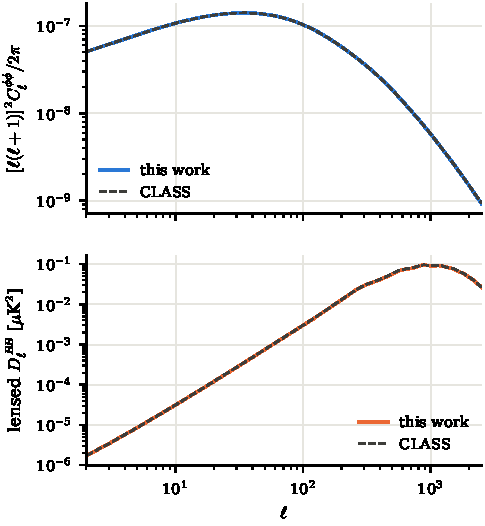
\includegraphics[width=\columnwidth]{m4_lensing}
\caption{\emph{Top:} lensing potential power spectrum. \emph{Bottom:} B-mode spectrum generated by lensing of the E
modes (no primordial B modes). Dashed: CLASS run with the same parameters.}
\label{fig:lensing}
\end{figure}

\begin{figure}
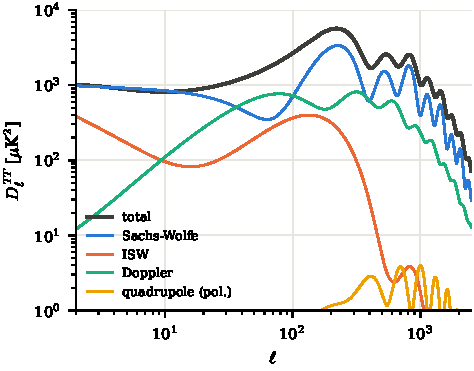
\includegraphics[width=\columnwidth]{m4_TT_components}
\caption{Contributions to the TT spectrum from the four terms of the source function~\eqref{eq:ST}, each computed
alone. They add in amplitude, not in power, so the cross terms make the total differ from the sum of the curves.}
\label{fig:TTcomp}
\end{figure}

\paragraph*{Decomposition.} Figure~\ref{fig:TTcomp} splits the TT spectrum into the four terms of Eq.~\eqref{eq:ST}:
\begin{itemize}
\item The SW term, $\Theta_0+\Psi$ at last scattering, dominates on all scales. It gives the plateau
      ($843\muK$ at $\ell=10$) and the acoustic peaks.
\item The Doppler term, from the baryon velocity at last scattering, is out of phase with the density by $\pi/2$. It
      fills in the troughs: at $\ell=400$ it is as large as the SW term. Its amplitude is reduced relative to the
      density term by $\sqrt{3}c_s/c=(1+R_b)^{-1/2}$, so the peaks remain visible. On the largest scales it vanishes,
      because the velocity is $\propto\kappa$ outside the horizon.
\item The ISW term has two parts:
      \begin{itemize}
      \item The early ISW effect comes from the potentials still decaying just after recombination, because radiation
            is not yet negligible. It adds power near the first peak ($270\muK$ at $\ell=220$), and since it adds
            coherently with the SW term, it raises the first peak considerably.
      \item The late ISW effect comes from the decay of $\Phi$ in the $\Lambda$ era. A photon crossing a decaying
            potential well gains more energy falling in than it loses climbing out. The potentials decay only on very
            large scales today, so the late ISW dominates the rise at the lowest multipoles ($385\muK$ at $\ell=2$). It is
            a direct signature of dark energy.
      \end{itemize}
\item The polarization/quadrupole term is very small, $\sim10^{-3}$ of the total.
\end{itemize}

\begin{figure}
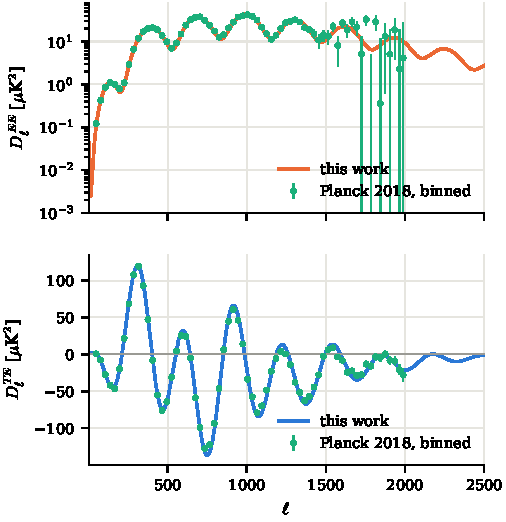
\includegraphics[width=\columnwidth]{m4_EE_TE}
\caption{$E$-mode polarization (\emph{top}) and temperature--polarization cross spectrum (\emph{bottom}) compared with
binned Planck 2018 data.}
\label{fig:EETE}
\end{figure}

\paragraph*{Polarization.} The EE and TE spectra (Fig.~\ref{fig:EETE}) agree well with Planck. Their shapes follow from
the fact that polarization is created by the quadrupole during the brief decoupling, $\Pi\propto(\kappa/\tau')\Theta_1$
(Sec.~\ref{sec:m3}):
\begin{itemize}
\item The $E$-mode peaks at $\ell=395$, 690, 994 and 1304 lie between the temperature peaks, close to the TT
      troughs, because they trace the velocity $\propto\sin(kr_s)$ rather than the density $\propto\cos(kr_s)$.
\item The EE amplitude grows from large to small scales up to $\ell\approx1000$, because the quadrupole is generated
      by free streaming over one mean free path, which is more effective for short wavelengths ($\propto k$). It then
      falls with the damping. The EE peaks are about 100 times lower than the TT peaks.
\item At $\ell\lesssim10$ the reionization bump ($D_\ell\approx0.04\muK$) comes from rescattering at $z\lesssim10$.
      The relevant quadrupole is the large-scale temperature anisotropy seen by the free electrons at reionization,
      and the horizon at $z=8$ projects to $\ell\sim$ a few. The amplitude scales as $\tau_{\rm reion}^2$, so this bump is
      the main handle on reionization.
\item The TE spectrum correlates the density and velocity terms, $\propto\cos(kr_s)\sin(kr_s)\propto\sin(2kr_s)$. It
      therefore changes sign twice as often as the TT peaks repeat: at $\ell=52$, 211, 401, 550, \dots. Its largest
      values are $+120\muK$ at $\ell=310$ and $-137\muK$ at $\ell=751$. The anti-correlation at $\ell\sim50$--$200$, on
      scales larger than the sound horizon, is a key signature that the fluctuations were adiabatic and present
      before they entered the horizon, as inflation predicts.
\end{itemize}

\begin{figure}
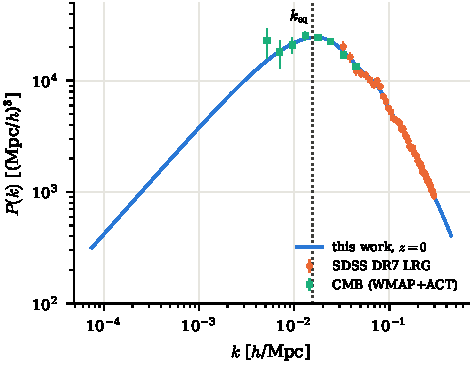
\includegraphics[width=\columnwidth]{m4_Pk}
\caption{Matter power spectrum today compared with the SDSS DR7 luminous red galaxy power spectrum~\cite{Reid2010} and
with the estimate from WMAP and ACT CMB data. The vertical dotted line marks $k_{\rm eq}$.}
\label{fig:Pk}
\end{figure}

\paragraph*{Matter power spectrum.} The matter power spectrum (Fig.~\ref{fig:Pk}) peaks at $k=0.0167\hMpc$ with
$P=2.46\times10^4\,(h^{-1}\Mpc)^3$, close to $k_{\rm eq}=0.0155\hMpc$ from Milestone~I. On large scales the slope is
$0.95\approx n_s$, the primordial spectrum. On small scales the spectrum falls as modes that entered during RD were
suppressed. Between $0.1$ and $0.4\hMpc$ the local slope is $-1.7$; the asymptotic $k^{n_s-4}\ln^2k$ is only reached at
much larger $k$. The peak is not sharp, because the transition from RD to MD is gradual.

The baryon acoustic oscillations appear as small wiggles at $k\sim0.05$--$0.3\hMpc$, with period
$2\pi/r_s(z_d)\approx0.064\hMpc$. They are the same sound waves as in the CMB, frozen into the baryon distribution at
the drag epoch, and then imprinted in the dark matter as the baryons fell into the dark matter wells. Their amplitude is
small because the baryons are only $16\%$ of the matter.

The model matches the CMB-derived points and the SDSS DR7 LRG spectrum, with $\chi^2=12.2$ for the 45 LRG points
(compared directly, without a free bias or amplitude parameter). The LRG data cover the turnover only partially, but
they clearly favour the decline at $k>k_{\rm eq}$ predicted by a universe dominated by cold dark matter. In a
baryon-only universe there would be no turnover near $k_{\rm eq}$ of this form, and the BAO wiggles would be large.

\begin{figure*}
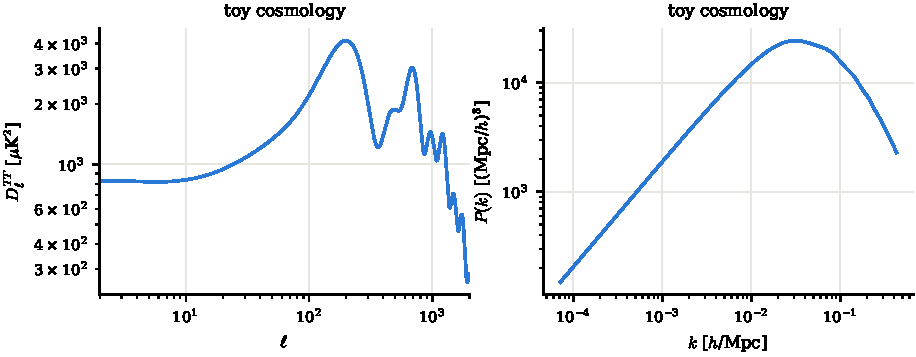
\includegraphics[width=\textwidth]{m4_toy}
\caption{TT spectrum (\emph{left}) and matter power spectrum (\emph{right}) for the toy cosmology of the course
reference figures ($h=0.7$, $\Om_b=0.05$, $\Om_{\rm CDM}=0.45$, $\Om_\Lambda=0.5$, no neutrinos, no helium, no
reionization, no polarization).}
\label{fig:toy}
\end{figure*}

\paragraph*{Toy cosmology.} As a cross-check with the reference figures of the course, we also ran a matter-heavy toy
model (Fig.~\ref{fig:toy}). The TT peaks are at $\ell=199$, 485 and 685, compared with $\approx199$, 491 and 690 read off
the reference figure. The differences from the fiducial model are what the physics above predicts:
\begin{itemize}
\item With $\Om_M=0.5$ and no neutrinos, equality is at $z\approx9900$ instead of 3400. The potentials have decayed
      less by recombination, so radiation driving and the early ISW effect are weaker.
\item The baryon loading term then dominates the peak heights, and the third peak is much higher than the second.
\item The peaks shift to lower $\ell$ because the larger matter density reduces the distance to the last-scattering
      surface ($\chi_*\approx11\,090\Mpc$, $20\%$ less) more than the sound horizon ($136\Mpc$, $6\%$ less), so
      $\ell_A\approx256$ instead of 303.
\item $P(k)$ peaks at $k=0.031\hMpc$, as expected from $k_{\rm eq}\propto\Om_M/\sqrt{\Om_r}$ in units of $h$/Mpc,
      which is larger by a factor 2.1.
\end{itemize}
The overall amplitude of both $C_\ell$ and $P(k)$ is a constant factor $\approx2.1$ higher than the reference. A constant
factor in both spectra is what a different $A_s$ would give, and the factor is consistent with the reference using
$A_s=10^{-9}$ (this is our inference; the reference does not state $A_s$).

% ===========================================================================
\section{Validation against CLASS}\label{sec:validation}
% ===========================================================================

As an end-to-end test, we ran CLASS~\cite{Lesgourgues2011,Blas2011} (through its Python wrapper) with the same
parameters and physics: massless neutrinos and the same tanh reionization, unlensed unless stated otherwise. This
section uses the Peebles recombination model of Sec.~\ref{sec:m2}; with RECFAST (Sec.~\ref{sec:recfast}), the
code's default, the recombination-driven differences below drop by an order of magnitude in TT and by a factor of four in EE. The comparison
(Fig.~\ref{fig:class}) is:
\begin{itemize}
\item \textbf{Background.} $H$, $t$ and $\eta$ agree to $\sim10^{-7}$. The age (13.8483\,Gyr) and $\eta_0$
      ($14\,191.6\Mpc$) agree in all printed digits.
\item \textbf{Recombination.} CLASS uses HyRec, which includes the multi-level atom and non-equilibrium helium
      recombination. Our $X_e$ agrees to $\sim0.1\%$ during hydrogen recombination. It differs by 3--4\% during
      He$^+$ recombination at $z\approx2000$--$2500$, where our Saha helium recombines too fast, and by $+15\%$ in the
      freeze-out tail. These differences have little effect on the observables:
      \begin{itemize}
      \item $z_*=1084.32$ versus $1084.70$, and $r_s(z_*)=144.90$ versus $144.87\Mpc$;
      \item $z_d=1059.83$ versus $1060.03$, and $r_s(z_d)=147.08$ versus $147.06\Mpc$;
      \item $\tau_{\rm reion}=0.0580$ versus $0.0578$.
      \end{itemize}
\item \textbf{Angular spectra.}
      \begin{itemize}
      \item TT agrees to $1.1\%$ for $2\le\ell\le2000$, and to $0.97\%$ for $\ell\le1200$.
      \item EE agrees to $1\%$ at $\ell=2$--8 and to $3.4\%$ for $\ell\ge100$. The largest difference, up to $+6\%$, is
            in the EE trough at $\ell\approx15$--20, where the spectrum is tiny.
      \item TE differs by at most $1.5\%$ of its peak amplitude.
      \end{itemize}
      When we remove helium from both codes, TT agrees to 0.3--0.9\%. The remaining differences are therefore mostly
      due to the recombination model, which changes the damping tail and the polarization amplitude.
\item \textbf{Matter power spectrum.} $P(k)$ agrees to $0.11\%$ for all $k$.
\item \textbf{Lensing.} To separate the lensing from the unlensed spectra we compare the ratio of lensed to unlensed
      spectra from each code, with CLASS run with lensing on and $\Delta\ell=500$ extra multipoles. The TT ratios
      agree to $1.2\times10^{-4}$ for $\ell\le1000$, $5.8\times10^{-4}$ for $\ell\le2000$ and $1.1\times10^{-3}$ for
      $\ell\le2500$. $C_\ell^{\phi\phi}$ agrees to $0.11\%$ for $\ell\le1000$ and $1.1\%$ up to $\ell=2500$, where our
      extrapolation of the Weyl potential beyond $k_{\max}$ takes over. The lensing B modes agree to $1.5\%$ for
      $\ell\le2000$ and $1.2\%$ up to $\ell=2500$. Fed with identical input spectra, our lensing module reproduces CLASS's lensed TT to $1.4\times10^{-4}$.
\end{itemize}

\begin{figure*}
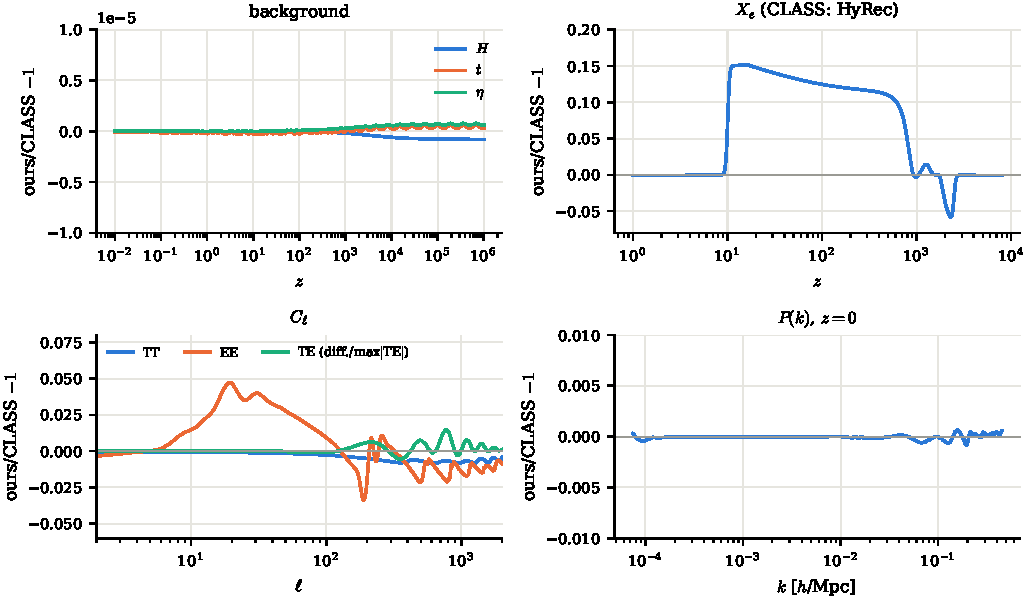
\includegraphics[width=0.9\textwidth]{validation_class}
\caption{Relative differences between our code and CLASS run with the same physics. \emph{Top left:} background
$H$, $t$ and $\eta$. \emph{Top right:} free electron fraction (CLASS uses HyRec). \emph{Bottom left:} unlensed TT
and EE spectra, and the TE difference relative to the maximum of $|C_\ell^{TE}|$. \emph{Bottom right:} matter power
spectrum today.}
\label{fig:class}
\end{figure*}

% ===========================================================================
\section{Extension: spatial curvature}\label{sec:curvature}
% ===========================================================================

The milestones assume a flat universe. As an extension we added spatial curvature to all modules. Curvature is
one of the main targets of the CMB: it changes the distance to the last-scattering surface, and therefore the angle
under which the acoustic scale appears. Throughout this section the matter, radiation and baryon densities are those
of the fiducial model, and $\Om_{\Lambda0}=1-\Om_{M0}-\Om_{r0}-\Om_{K0}$ absorbs the change.

\subsection{Theory}

\paragraph*{Background.} With $K=-\Om_{K0}H_0^2/c^2$ ($K<0$ open, $K>0$ closed), the Friedmann equation already
contains the curvature term $\Om_{K0}e^{-2x}$. Distances use the comoving transverse distance
$r=\sin_K(\chi)\equiv\sin(\sqrt K\chi)/\sqrt K$, $\chi$, or $\sinh(\sqrt{-K}\chi)/\sqrt{-K}$ for closed, flat and open
space. In a closed universe light rays from a point converge again, so objects at fixed $\chi$ look larger; in an open
universe they diverge and objects look smaller.

\paragraph*{Perturbations.} In curved space the plane waves $e^{i\bm k\cdot\bm x}$ are replaced by eigenfunctions of
the Laplacian, $\nabla^2G=-k^2G$. It is convenient to label them by $q^2=k^2+K$ and $\nu=q/\sqrt{|K|}$. In an open
universe every $q>0$ is allowed. A closed universe is finite, so the spectrum is discrete: only integer $\nu\ge3$
describe scalar perturbations ($\nu=1$ is a homogeneous change of the background and $\nu=2$ is a pure gauge
mode). Three changes follow in the equations of
Milestone~III~\cite{HuSeljak1998,Lesgourgues2014}:
\begin{itemize}
\item The $00$ Einstein equation contains $k^2-3K$ instead of $k^2$: curvature adds to the potential energy of a
      perturbation. The same factor appears in the Poisson equation for $\Delta_M$.
\item The free-streaming couplings between neighbouring multipoles of photons, polarization and neutrinos carry the
      factors $s_\ell=\sqrt{1-(\ell^2-1)K/k^2}$:
      $\Theta_\ell'=\frac{\kappa}{2\ell+1}[\ell s_\ell\Theta_{\ell-1}-(\ell+1)s_{\ell+1}\Theta_{\ell+1}]+\dots$. Geometrically,
      the angle subtended by a wavelength changes along the line of sight. In a closed universe $s_\nu=0$, so the
      hierarchy of mode $\nu$ ends at $\ell=\nu-1$: a finite space has no structure on angles smaller than its modes
      allow. In this convention the physical shear is $\Theta_2/s_2$, which enters $\Psi$.
\item The truncation of the hierarchies uses $\cot_K(\eta)$ instead of $1/\eta$.
\end{itemize}
The initial conditions are those of the flat case, since curvature is negligible at $x=-18$, and we keep the
normalization $\mathcal{R}=1$ and $\mathcal{P}_{\mathcal{R}}=A_s(k/k_{\rm pivot})^{n_s-1}$, as in CLASS.

\paragraph*{Hyperspherical Bessel functions.} The projection of a mode onto the sky now uses the radial
eigenfunctions $\Phi^\nu_\ell(\chi)$ (with $\chi$ in units of the curvature radius) instead of $j_\ell(kr)$. They obey
\begin{equation}
\Phi''+2\cot_K\chi\,\Phi'+\Big[\nu^2-{\rm sgn}K-\frac{\ell(\ell+1)}{\sin_K^2\chi}\Big]\Phi=0,
\end{equation}
with $\Phi^\nu_0=\sin(\nu\chi)/(\nu\sin_K\chi)$ and the three-term recurrence
\begin{align}
\sqrt{\nu^2-{\rm sgn}K(\ell+1)^2}\,\Phi_{\ell+1} &= (2\ell+1)\cot_K\chi\,\Phi_\ell \nonumber\\
 &\quad -\sqrt{\nu^2-{\rm sgn}K\,\ell^2}\,\Phi_{\ell-1}.
\end{align}
They reduce to $j_\ell(\nu\chi)$ for $\nu\to\infty$. The line-of-sight integral no longer allows the integrations by
parts used in Eq.~\eqref{eq:ST}, so we project the three parts of the source separately:
\begin{align}
\Theta_\ell(k) &= \int\dd x\,\Big[S_{T0}\Phi_\ell + S_{T1}\frac{\sqrt{|K|}}{k}\Phi_\ell' \nonumber\\
 &\qquad + S_{T2}\frac{3(|K|/k^2)\Phi_\ell''+\Phi_\ell}{2s_2}\Big],\\
\Theta^E_\ell(k) &= \sqrt{\tfrac{(\ell+2)!}{(\ell-2)!}}\int\dd x\,\frac{3\gt\,\Pi}{4}\,\frac{\Phi_\ell}{s_2(kr)^2},
\end{align}
with $S_{T0}=\gt(\Theta_0+\Psi)+e^{-\tau}(\Psi'-\Phi')$, $S_{T1}=-\gt v_b$ and $S_{T2}=\gt\Pi/2$. In the flat limit
these are $j_\ell$, $j_\ell'$ and $(3j_\ell''+j_\ell)/2$, and integrating by parts recovers Eq.~\eqref{eq:ST}. In a
closed universe the $k$-integral of Eq.~\eqref{eq:cl} becomes a sum over integer $\nu$.

\subsection{Implementation and tests}

$\Phi^\nu_\ell$ is computed by upward recurrence~\cite{Kosowsky1998,Tram2017} below the turning point
$\ell(\ell+1)=(\nu^2-{\rm sgn}K)\sin_K^2\chi$, where it oscillates, and by Miller's downward recurrence above it, where
it decays exponentially; in a closed universe the downward recurrence starts exactly at $\ell=\nu-1$. The functions
agree with $j_\ell$ in the flat case to $2\times10^{-12}$, satisfy the radial equation to the accuracy of the finite
differences, match the closed-form Gegenbauer polynomials of a closed universe to $10^{-13}$, and approach
$j_\ell(\nu\chi)$ as $1/\nu^2$.

The perturbations are sampled in $q$; in a closed universe only integer $\nu$ are used, and in an open universe the
grid extends down to $q=0.01\sqrt{|K|}$, since the modes near the curvature scale contribute to the lowest multipoles.
For each mode and each point on the line of sight we compute $\Phi_0\dots\Phi_{\ell_{\rm cap}}$, where $\ell_{\rm cap}$ is
just beyond the turning point. One subtlety concerned the closed-universe sum. Rounding a uniform $k$-grid to integer
$\nu$ gives an irregular stride of 2--3 in $\nu$, while $\Theta_\ell^2$ oscillates with a period of only a few units of
$\nu$. The trapezoidal rule then loses the high accuracy it has for oscillating integrands on a uniform grid, and $C_\ell$
was off by up to $4\%$. A uniform integer stride fixes this. With the flat Bessel functions the same code reproduces the
integrated-by-parts flat result to $5\times10^{-5}$, which tests the decomposition of the source. Two speed-ups bring the curved
line-of-sight integration from $\approx48$\,s to 26--42\,s on two cores for $\ell\le2000$ (7\,s with the flat
tables). First, modes with smaller $q$ use a proportionally coarser $x$-grid away from recombination (the radial
functions oscillate more slowly), but never coarser than $\Delta x=0.01$, which resolves reionization; this changes
$C_\ell$ by $<3\times10^{-5}$. Second, for $\nu\ge4000$ we use the flat approximation of CLASS: $\Phi^\nu_\ell(\chi)$ is
replaced by $j_\ell$ with the argument rescaled to put its turning point at $\chi_{\rm tp}$ and an empirical amplitude
correction~\cite{Lesgourgues2014}, read from tables of $j_\ell$ and $j_\ell'$. It is accurate near the turning point
but drifts in phase far beyond it. Since those oblique projections carry little weight for Silk-damped modes, the
effect on $C_\ell$ is $\lesssim6\times10^{-4}$ at $\Om_K=\pm0.05$, where a third of the modes use it. For
$|\Om_K|=0.2$ no mode reaches $\nu=4000$ below $k=0.3\Mpc^{-1}$, and lowering the threshold quickly costs accuracy
($0.4\%$ for $\nu\ge2000$, $1\%$ for $\nu\ge1000$).

\subsection{Results}

\begin{figure}
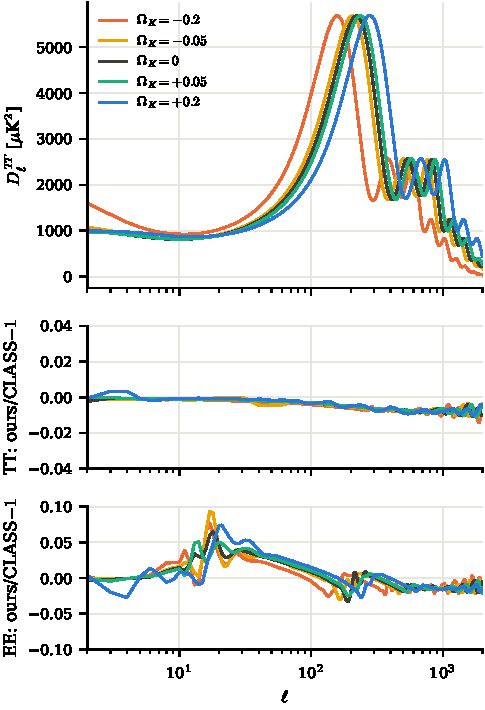
\includegraphics[width=\columnwidth]{curvature_spectra}
\caption{\emph{Top:} TT spectra for $\Om_K=-0.2$, $-0.05$, 0, 0.05 and 0.2 at fixed matter and baryon density.
\emph{Middle and bottom:} TT and EE relative to CLASS run with the same physics (unlensed).}
\label{fig:curvature}
\end{figure}

\begin{table}
\caption{Curved models: the first TT peak from our code and from CLASS, the acoustic scale $\ell_A=\pi r(\chi_*)/r_s$,
and the largest TT difference from CLASS for $30\le\ell\le2000$.}
\label{tab:curvature}
\begin{ruledtabular}
\begin{tabular}{rcccccc}
$\Om_K$ & $\Om_\Lambda$ & $\ell_{\rm peak}$ & CLASS & $\ell_A$ & $\ell_{\rm peak}/\ell_A$ & TT diff. \\
\hline
$-0.20$ & 0.883 & 158 & 158 & 215.7 & 0.732 & 1.4\% \\
$-0.05$ & 0.733 & 206 & 206 & 280.8 & 0.734 & 1.1\% \\
$0$     & 0.683 & 221 & 221 & 301.7 & 0.733 & 1.1\% \\
$+0.05$ & 0.633 & 236 & 236 & 322.2 & 0.733 & 1.2\% \\
$+0.20$ & 0.483 & 279 & 280 & 381.4 & 0.731 & 1.0\% \\
\end{tabular}
\end{ruledtabular}
\end{table}

Figure~\ref{fig:curvature} and Table~\ref{tab:curvature} show the result. Our spectra agree with CLASS as well in
curved as in flat models: TT to $0.15$--$0.35\%$ for $\ell\le30$ and $1$--$1.4\%$ up to $\ell=2000$, EE to $2$--$3\%$ for
$\ell\ge100$, and $P(k)$ to $0.12\%$ for $k>10^{-3}\Mpc^{-1}$ ($\Om_K=\pm0.05$). The background agrees to $10^{-6}$ and the potentials
today to $\sim10^{-5}$. The remaining differences are the same as in the flat case and come from the recombination
model.

The main effect of curvature is geometric. The physics at recombination is unchanged, because curvature is negligible
then, so the sound horizon is the same in all models to $0.05\%$ ($r_s=144.82$--$144.89\Mpc$; the small spread comes
from the optical depth to reionization, which shifts the $\tau=1$ surface). What changes is the transverse distance to the last-scattering surface, $r(\chi_*)$: it is
smaller in a closed universe, where light rays focus, and larger in an open one. The whole acoustic pattern therefore
shifts in $\ell$. The ratio $\ell_{\rm peak}/\ell_A$ is $0.731$--$0.734$ in all five models, so the first peak follows the
geometric prediction, while $\Om_K=\mp0.2$ moves it by $-29\%$ and $+26\%$. A measurement of the peak positions
therefore measures $r(\chi_*)/r_s$, which is why the CMB constrains curvature so well once $\Om_Mh^2$ is fixed by the
peak heights.

The low multipoles change too. In the closed model with $\Om_K=-0.2$ the larger $\Om_\Lambda=0.88$ makes the potentials
decay earlier and more strongly, and the late ISW effect raises $D_2$ to $1600\muK$ against $1020\muK$ in the flat
model. In the open models the opposite change in $\Om_\Lambda$ is partly compensated by curvature itself, which also
makes the potentials decay once it dominates the expansion. These large-scale effects are limited by cosmic variance,
and in practice the geometric degeneracy between $\Om_K$ and $\Om_\Lambda$ is broken by combining the CMB with
lensing or BAO.

% ===========================================================================
\section{Extension: massive neutrinos}\label{sec:neutrinos}
% ===========================================================================

Neutrino oscillations show that at least two neutrino species are massive, with $\sum m_\nu\gtrsim0.06$\,eV. For
cosmology the masses matter because the neutrinos become non-relativistic in the late universe: before that they
behave like radiation, afterwards like a hot component of the dark matter that does not cluster on small scales. We
add one massive species of mass $m_\nu$ (the minimal normal-ordering case, if the lighter ones are treated as
massless), following Refs.~\cite{Ma1995,LesgourguesTram2011,LesgourguesPastor2006}. As in CLASS, its temperature
today is $T_{\nu}=0.71611\,T_{\rm CMB}$, which gives $\Om_\nu h^2=m_\nu/93.14$\,eV and contributes $1.0132$ to
$N_{\rm eff}$; the other $N_{\rm eff}-1.0132=2.0328$ species stay massless. We keep $h$, $\omega_b$ and $\omega_{\rm cdm}$
of the fiducial model, so that $\Om_\Lambda$ absorbs the neutrino density.

\subsection{Theory}

\paragraph*{Background.} The neutrinos decoupled at $T\sim1$\,MeV while relativistic, so their distribution keeps the
relativistic Fermi--Dirac form $f_0(q)=1/(e^q+1)$ in the comoving momentum $q=ap/(k_BT_{\nu})$, even after they
become non-relativistic. With $M(a)=am_\nu c^2/(k_BT_{\nu})$ the comoving energy is $\epsilon=\sqrt{q^2+M^2}$, and
\begin{align}
\rho_\nu&=\frac{15}{\pi^4}\Big(\frac{T_\nu}{T_{\rm CMB}}\Big)^4\frac{\rho_{\gamma0}}{a^4}\int_0^\infty dq\,q^2\epsilon f_0,\\
p_\nu&=\frac{15}{\pi^4}\Big(\frac{T_\nu}{T_{\rm CMB}}\Big)^4\frac{\rho_{\gamma0}}{a^4}\int_0^\infty dq\,\frac{q^4}{3\epsilon}f_0 .
\end{align}
For $M\ll1$ this is radiation ($p=\rho/3$, $\rho\propto a^{-4}$); for $M\gg1$, $\rho\to\frac{3\zeta(3)}{2}M$ times the
prefactor, i.e.\ matter with $\rho\propto a^{-3}$. The transition, $M\approx3$, happens at $1+z\approx M_0/3$, i.e.\
$z_{\rm nr}=118$, 296 and 594 for $m_\nu=0.06$, 0.15 and 0.3\,eV (Fig.~\ref{fig:nu}a). The derivatives needed for
$\mathcal H'$ and $\mathcal H''$ follow from $\rho'=-3(\rho+p)$ and $p'=-(5p-\mathfrak p)$, where
$\mathfrak p=\frac{15}{\pi^4}(\dots)\int dq\,q^6f_0/(3\epsilon^3)$ is the ``pseudo-pressure''. We evaluate the
integrals with 48-point Gauss--Laguerre quadrature, accurate to $10^{-7}$; age and conformal time agree with CLASS in
all printed digits.

\paragraph*{Perturbations.} A massive particle's velocity, $q/\epsilon$, depends on its momentum, so the perturbation
cannot be described by a single temperature multipole hierarchy. Following Ma and Bertschinger~\cite{Ma1995} we write
$f=f_0(q)[1+\Psi(\bm k,\hat n,q,\eta)]$ and expand $\Psi$ in Legendre multipoles $\Psi_\ell(q)$ for a set of momenta
$q_i$. In our variables ($\kappa=ck/\mathcal H$, Newtonian gauge),
\begin{align}
\Psi_0' &= -\kappa\frac{q}{\epsilon}\Psi_1+\Phi'\frac{d\ln f_0}{d\ln q},\\
\Psi_1' &= \frac{\kappa}{3}\frac{q}{\epsilon}\big(\Psi_0-2\Psi_2\big)-\frac{\kappa}{3}\frac{\epsilon}{q}\Psi\frac{d\ln f_0}{d\ln q},\\
\Psi_\ell' &= \frac{\kappa}{2\ell+1}\frac{q}{\epsilon}\big[\ell\Psi_{\ell-1}-(\ell+1)\Psi_{\ell+1}\big],\quad \ell\ge2 .
\end{align}
The free-streaming terms are those of massless neutrinos with $c$ replaced by the particle velocity $cq/\epsilon$,
and the metric terms act through $d\ln f_0/d\ln q$: a potential well shifts all momenta, which changes $f$ in
proportion to its slope. The neutrinos enter the Einstein equations through their density, velocity and shear,
\begin{align}
\delta\rho_\nu&\propto\int dq\,q^2\epsilon f_0\Psi_0,\nonumber\\
(\rho+p)_\nu\theta_\nu&\propto k\int dq\,q^3f_0\Psi_1,\nonumber\\
(\rho+p)_\nu\sigma_\nu&\propto\frac23\int dq\,\frac{q^4}{\epsilon}f_0\Psi_2,
\end{align}
which replace $4\rho_\nu\mathcal N_0$ and the shear of $\mathcal N_2$ in Eqs.~\eqref{eq:einstein1}--\eqref{eq:einstein2}. For
$M\to0$ and $\Psi_\ell=-\mathcal N_\ell\,d\ln f_0/d\ln q$ the system reduces exactly to the massless one, which also
gives the adiabatic initial conditions. We use 8 Gauss--Laguerre momenta and $\ell_{\max}=17$ (as CLASS); 16 momenta
or $\ell_{\max}=25$ change $C_\ell$ and $P(k)$ by less than $3\times10^{-5}$.

\paragraph*{Fluid approximation.} Deep inside the horizon ($k\eta>31$) the hierarchy is replaced by the fluid
equations of Ref.~\cite{LesgourguesTram2011} for $\delta_\nu$, $\theta_\nu$ and $\sigma_\nu$, with the adiabatic sound
speed $c_a^2=\frac{w}{3(1+w)}(5-\mathfrak p/p)$ and a viscosity closure for the shear, as in CLASS. This reduces the
system from 190 to 49 variables. Compared with the full hierarchy it changes $P(k)$ by up to 0.3\% at
$m_\nu=0.3$\,eV; CLASS's fluid approximation has the same error, to $10^{-4}$. With 190 variables the
dense linear algebra of the implicit (BDF) solver makes it about 20 times slower than an explicit Runge--Kutta
method, which gives identical results while the hierarchy is active; we use the explicit method there. A run with
massive neutrinos then takes 40--43\,s for the perturbations on 2 cores, compared with 37\,s for massless neutrinos.

\paragraph*{Matter power spectrum.} With massive neutrinos the total matter is CDM, baryons and neutrinos. We compute
the comoving density contrast directly,
$\Delta_m=\sum_i\rho_i[\delta_i-3(1+w_i)\mathcal Hv_i/(ck)]/\sum_i\rho_i$, which is the synchronous-gauge $\delta_m$
used by CLASS; for massless neutrinos it agrees with the Poisson equation~\eqref{eq:DeltaM} up to radiation terms of
order $10^{-3}$ at $k\sim10^{-4}\Mpc^{-1}$, and reduces the difference from CLASS there from $2\times10^{-3}$ to
$10^{-5}$. We also output the CDM+baryon spectrum $P_{cb}$, the relevant one for galaxy clustering.

\begin{figure*}
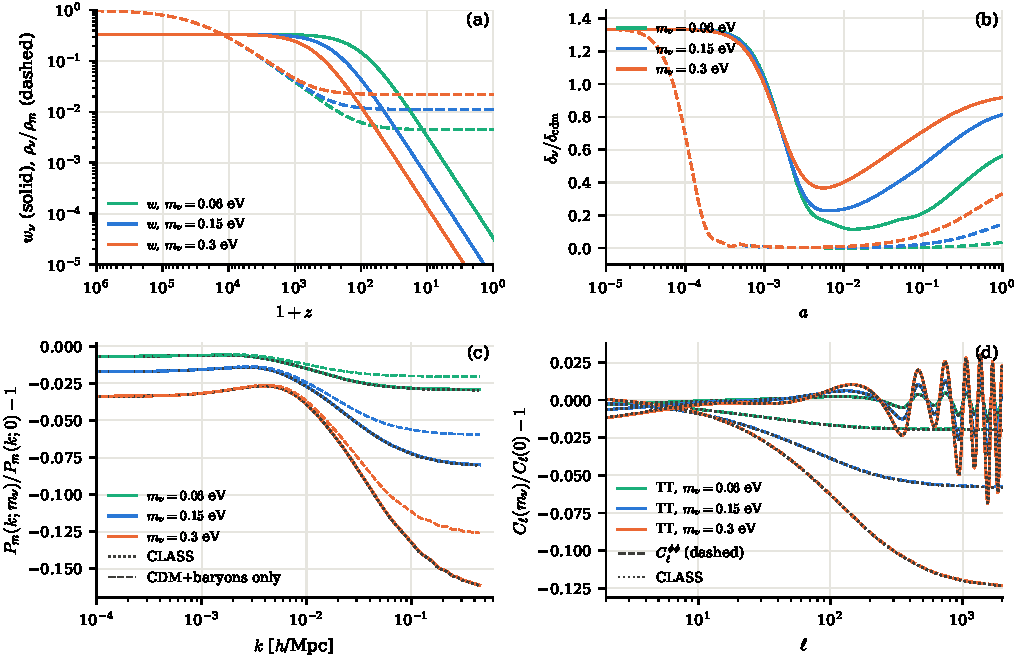
\includegraphics[width=0.95\textwidth]{neutrinos}
\caption{Massive neutrinos with $m_\nu=0.06$, 0.15 and 0.3\,eV (fixed $h$, $\omega_b$, $\omega_{\rm cdm}$).
\emph{(a)} Equation of state $w_\nu$ and density relative to all matter. \emph{(b)} $\delta_\nu/\delta_{\rm cdm}$ for
$k=0.01\Mpc^{-1}$ (solid) and $0.1\Mpc^{-1}$ (dashed): below the free-streaming scale the neutrinos stop clustering, and fall back into the CDM wells after they
slow down. \emph{(c)} Change of the total matter power spectrum (solid) and of the CDM+baryon spectrum (dashed)
today, with CLASS (dotted). \emph{(d)} Change of the unlensed TT spectrum (solid) and the lensing potential (dashed),
with CLASS (dotted).}
\label{fig:nu}
\end{figure*}

\subsection{Results}

\paragraph*{Free streaming.} While relativistic, neutrinos stream out of any structure smaller than the horizon.
After $z_{\rm nr}$ their thermal velocity $\langle v\rangle\approx3.15\,k_BT_\nu/(m_\nu a)$ decays, and the
free-streaming scale, the distance travelled in a Hubble time, shrinks. Its comoving wavenumber
$k_{\rm fs}\sim\sqrt{3/2}\,\mathcal H/\langle v\rangle$ grows as $a^{1/2}$ in matter domination; the smallest value
reached, at $z_{\rm nr}$, is $k_{\rm nr}\approx0.018\sqrt{\Om_m m_\nu/{\rm eV}}\,h\Mpc^{-1}\approx0.003$--$0.006\,h\Mpc^{-1}$.
Figure~\ref{fig:nu}b shows the consequence. Initially $\delta_\nu=\frac43\delta_{\rm cdm}$ (adiabatic). When a mode
enters the horizon the neutrino perturbation decays by free streaming. Later, when $k<k_{\rm fs}(a)$, the neutrinos
fall into the CDM potential wells and $\delta_\nu\to\delta_{\rm cdm}$: at $k=0.01\Mpc^{-1}$ this has largely happened
today for 0.3\,eV, but at $k=0.1\Mpc^{-1}$ the neutrinos still lag far behind.

\paragraph*{Matter power spectrum.} On scales above $k_{\rm nr}$ neutrinos behave like CDM, and $P(k)$ changes only
by $0.6$--3\% because $\Om_\Lambda$ is smaller (Fig.~\ref{fig:nu}c). Below the free-streaming scale the spectrum is
suppressed, by $2.9\%$, $8.0\%$ and $16.1\%$ at $k=0.5\,h\Mpc^{-1}$ for the three masses (CLASS: 3.0, 8.0, 16.2\%).
There are two reasons~\cite{HuEisensteinTegmark1998,LesgourguesPastor2006}. First, a fraction
$f_\nu=\Om_\nu/\Om_m=0.0045$, 0.011, 0.022 of the matter does not cluster, which removes $2f_\nu$ from
$P_m\propto[(1-f_\nu)\delta_{cb}]^2$. Second, the CDM and baryons grow more slowly, since only a fraction $1-f_\nu$ of
the matter falls into the wells: $\delta_{cb}\propto a^{1-3f_\nu/5}$ instead of $a$, which accumulates to a
suppression of $P_{cb}$ of several $f_\nu$. Together the suppression is $\approx-8f_\nu$ asymptotically; at
$k=0.5\,h\Mpc^{-1}$ we find $-6.5f_\nu$, $-7.1f_\nu$ and $-7.3f_\nu$. The CDM+baryon spectrum shows only the second
effect. This step-like suppression is why galaxy surveys are sensitive to $\sum m_\nu$.

\paragraph*{CMB.} The masses we consider make the neutrinos non-relativistic well after recombination, so the
primary anisotropies change only through the background. The extra matter today shortens the distance to the
last-scattering surface ($\eta_0$ decreases by 118\,Mpc for 0.3\,eV), which moves the peaks to lower $\ell$ (the
first from 221 to 219) and causes the oscillating residuals in Fig.~\ref{fig:nu}d. The lower $\Om_\Lambda$ reduces
the late ISW effect, and for 0.3\,eV the neutrinos are no longer fully relativistic at decoupling, which changes the
early ISW effect. The lensing potential, a projection of the matter distribution, is suppressed like $P(k)$: at
$\ell=1000$ by 1.9\%, 5.7\% and 12.0\%. CMB lensing therefore constrains the neutrino mass: through the smoothing of the peaks
(Sec.~\ref{sec:lensing}) and through direct reconstructions of $C_\ell^{\phi\phi}$.

\paragraph*{Validation.} We compare the effect of the mass, $X(m_\nu)/X(0)-1$, with CLASS run with the same
parameters (which removes the recombination differences of Sec.~\ref{sec:validation}). For $m_\nu=0.06$\,eV, the
effects on TT, lensed TT, $C_\ell^{\phi\phi}$ and $P_m$ agree to $3$--$5\times10^{-4}$ and on EE to $6\times10^{-4}$;
for 0.3\,eV to $8\times10^{-4}$, $1.0\times10^{-3}$, $3\times10^{-4}$, $4\times10^{-4}$ and $3.7\times10^{-3}$, i.e.\
better than 3\% of the effect itself. A nearly massless species ($m_\nu=10^{-4}$\,eV) reproduces the massless
neutrinos to $4\times10^{-7}$ in $\Phi$ at recombination when the same $\ell_{\max}$ is used.

% ===========================================================================
\section{Extension: two-point functions}\label{sec:twopoint}
% ===========================================================================

Power spectra are the natural output of a Boltzmann code, because each Fourier mode or multipole evolves
independently in linear theory. Observers often measure the equivalent real-space two-point functions instead. They
show localized features, such as the acoustic scale or the BAO peak, as features at one separation, and they are
easier to estimate on a masked sky or in a survey with complicated geometry. We added functions that compute the
angular correlation functions of the CMB, the three-dimensional correlation function of the matter, and the angular
power spectrum and correlation function of the matter (or galaxy) density projected over a redshift distribution.

\subsection{Theory}

\paragraph*{Angular correlation functions.} For a statistically isotropic field on the sphere,
$a_{\ell m}$ are uncorrelated with variance $C_\ell$, and the addition theorem
$\sum_mY_{\ell m}(\hat n)Y^*_{\ell m}(\hat n')=\frac{2\ell+1}{4\pi}P_\ell(\hat n\cdot\hat n')$ gives
\begin{equation}
C(\theta)=\langle T(\hat n)T(\hat n')\rangle=\sum_\ell\frac{2\ell+1}{4\pi}C_\ell B_\ell^2P_\ell(\cos\theta),
\label{eq:Ctheta}
\end{equation}
with an optional Gaussian beam $B_\ell=e^{-\ell(\ell+1)\sigma_b^2/2}$. The polarization is a spin-2 field, so its
correlation functions involve the Wigner functions $d^\ell_{mm'}$ of Sec.~\ref{sec:lensing}. With $Q$ and $U$ measured
relative to the great circle joining the two points~\cite{Challinor2005},
$\xi_\pm=\langle QQ\rangle\pm\langle UU\rangle=\sum_\ell\frac{2\ell+1}{4\pi}(C_\ell^{EE}\pm C_\ell^{BB})d^\ell_{2,\pm2}$
and $\xi_X=\langle TQ\rangle=\sum_\ell\frac{2\ell+1}{4\pi}C_\ell^{TE}d^\ell_{20}$. We sum
$\ell=2$--2500 (the monopole and dipole are not cosmological) with the Legendre and Wigner recurrences.

\paragraph*{Matter correlation function.} In three dimensions the transform is
\begin{align}
\xi(r)&=\int_0^\infty\frac{k^2dk}{2\pi^2}P(k)j_0(kr)\nonumber\\
&=\frac{1}{2\pi^2r}\int_0^\infty dk\,kP(k)\sin(kr).
\end{align}
The integrand oscillates many times for $r\sim100\Mpc$, so we use Filon's method~\cite{Filon1929}: $kP(k)$ is
interpolated linearly in $k$ between tabulated points and the product with $\sin(kr)$ is integrated analytically. The
grid then only has to resolve $P(k)$, including its BAO wiggles (we use $d\ln k=0.002$ and $dk\le5\times10^{-4}\Mpc^{-1}$
below $1\Mpc^{-1}$), for all $r$ at once. The integral needs $P(k)$ up to $k\sim10\Mpc^{-1}$. Beyond the computed range
we extrapolate $\Delta_M\propto k^2T(k)$ with the shape of the no-wiggle transfer function of
Ref.~\cite{EisensteinHu1998} anchored at $k_{\max}$ (accurate to 1.5\% up to $20\Mpc^{-1}$ from $k_{\max}=0.3\Mpc^{-1}$),
and $\Delta_M\propto k^2$ below $k_{\min}$. We also compute $\sigma_R$, the rms of $\Delta_M$ in top-hat spheres, and
$\sigma_8$.

\paragraph*{Projected density.} A galaxy survey with redshift distribution $n(z)$ and linear bias $b$ sees the
projected field $\delta_g(\hat n)=\int d\chi\,W(\chi)\,b\,\Delta_M(\chi\hat n,\chi)$ with $W=n(z)\,dz/d\chi$ normalized to
unit integral. Expanding the plane waves in spherical harmonics, as for the CMB (Sec.~\ref{sec:m4}),
\begin{align}
C_\ell&=4\pi\int\frac{dk}{k}\mathcal P_{\mathcal R}(k)\Delta_\ell(k)^2,\nonumber\\
\Delta_\ell(k)&=\int d\chi\,W(\chi)\,b\,\Delta_M(k,\chi)\,j_\ell(k\chi).
\label{eq:clgal}
\end{align}
For $\ell\gg1$, $j_\ell(k\chi)$ picks out $k\chi\approx\ell+\frac12$, and Eq.~\eqref{eq:clgal} reduces to the Limber
approximation~\cite{Limber1953,LoVerde2008},
$C_\ell=\int d\chi\,W^2b^2P((\ell+\frac12)/\chi,\chi)/\chi^2$: the multipole $\ell$ probes the transverse wavenumber
$k=(\ell+\frac12)/\chi$ at each distance. The Limber approximation drops the radial modes, which matter when the window is
not much wider than the wavelength. For $\sigma_z=0.1$ at $z=1$ it is 4\% wrong at $\ell=20$ and 0.4\% at $\ell=100$, so we
use the exact projection below $\ell=200$ (with all $j_\ell$ for one $k\chi$ from a single recurrence) and Limber
above. We include only the density term: redshift-space distortions, lensing magnification and the relativistic
corrections are left out, and $P(k)$ is linear. The angular correlation function $w(\theta)$ follows from
Eq.~\eqref{eq:Ctheta}; small angles need $\ell$ up to $\sim3\times10^4$ (Limber on a logarithmic grid, with a cosine
taper at the end to avoid ringing from the truncation).

\begin{figure*}
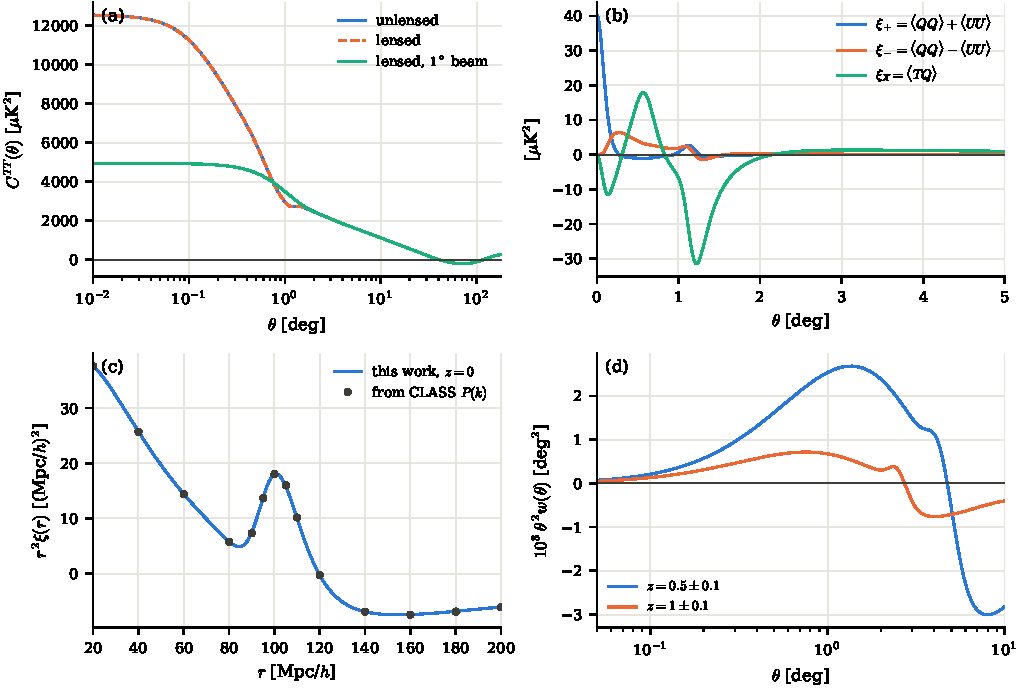
\includegraphics[width=0.95\textwidth]{twopoint}
\caption{Two-point functions of the fiducial model. \emph{(a)} CMB temperature correlation function, unlensed,
lensed, and lensed with a $1^\circ$ beam. \emph{(b)} Polarization correlation functions (unlensed). \emph{(c)}
Matter correlation function today, with the BAO peak; points are the transform of CLASS's $P(k)$. \emph{(d)} Angular
correlation function of the matter projected over Gaussian redshift distributions ($\sigma_z=0.1$, $b=1$).}
\label{fig:twopoint}
\end{figure*}

\subsection{Results}

\paragraph*{CMB.} The variance of the temperature is $C(0)=12\,550\muK$, i.e.\ $112\,\mu$K rms (Fig.~\ref{fig:twopoint}a).
The correlation falls to half at $\theta\approx0.5^\circ$, the angle subtended by the scales of the first acoustic peak,
and shows a shoulder near $1^\circ$. This is the real-space counterpart of the acoustic peaks: the sound horizon
subtends $\theta_*=r_s/\chi_*=0.60^\circ$, and a localized initial perturbation produces a ring of that radius around
itself. At large angles $C(\theta)$ is set by the lowest multipoles. It crosses zero at $41^\circ$ and $117^\circ$, with
$-205\muK$ at $72^\circ$ and $+259\muK$ at $180^\circ$. Because only a few multipoles contribute, the cosmic variance
of $C(\theta)$ is large here; the observed sky shows almost no correlation above $60^\circ$, one of the known
large-angle anomalies. Lensing changes $C(\theta)$ by at most $6\muK$ (at $1.1^\circ$, where it smooths the acoustic
shoulder), and conserves the variance to $10^{-4}$, since it only remaps the sky. A $1^\circ$ beam reduces the variance
to $4\,940\muK$. The polarization has rms $\sqrt{\xi_+(0)}=6.3\,\mu$K (Fig.~\ref{fig:twopoint}b). The
temperature--polarization correlation $\xi_X$ is $+18\muK$ at $0.57^\circ$ and $-31\muK$ at $1.22^\circ$: around a
temperature hot spot the polarization alternates between radial and tangential. This pattern comes from the flow of
the photon--baryon fluid into and out of the potential wells at decoupling, and it has been seen by stacking hot
spots in the WMAP data~\cite{Komatsu2011}.

\paragraph*{Matter.} The matter correlation function (Fig.~\ref{fig:twopoint}c) has the BAO peak at
$r=100.5\,h^{-1}\Mpc=150\Mpc$, close to the sound horizon at the drag epoch, $r_d=147\Mpc$ (the smooth decline of
$\xi$ moves the maximum of $r^2\xi$ slightly outward). Each initial point perturbation launches a spherical sound wave
in the photon--baryon fluid that stalls at $r_d$ when the baryons are released, so the baryons, and the dark matter
that later falls into them, end up with a shell at $r_d$ around every overdensity~\cite{Eisenstein2005}. In Fourier
space this single feature appears as the series of BAO wiggles. We find $\sigma_8=0.82071$ (CLASS: 0.82068). Our
$\xi(r)$ agrees with the transform of CLASS's $P(k)$ (computed independently with adaptive quadrature) to
$3\times10^{-4}$ at $r=20\,h^{-1}\Mpc$, and to 0.9\% of the BAO peak height of $r^2\xi$ for $r\ge60\,h^{-1}\Mpc$. The
latter is not numerical, as the transform reproduces analytic and quadrature results to $10^{-6}$ and $7\times10^{-4}$ in
the unit tests. It comes from the $\pm7\times10^{-4}$ oscillating difference between the two $P(k)$, which follows
the BAO phase (Sec.~\ref{sec:validation}): the BAO peak in $\xi$ is a small residual of a large cancellation, and it is
sensitive to the damping and phase of the wiggles.

\paragraph*{Projected density.} For Gaussian redshift distributions at $z=0.5$ and 1 ($\sigma_z=0.1$), our $C_\ell$ agree
with CLASS's number-count spectra (density term only, exact projection) to $7\times10^{-4}$ and $1.7\times10^{-3}$ for
$\ell\le500$, and to $1.9\times10^{-3}$ for $500<\ell\le2000$ (computed with $k_{\max}=1\Mpc^{-1}$; with the default
$0.3\Mpc^{-1}$ the extrapolated $P(k)$ misses the residual BAO wiggles, which costs up to 1.5\% at $\ell=1000$--2000). In $w(\theta)$
(Fig.~\ref{fig:twopoint}d) the BAO shell appears at the angle $r_d/\chi(z)$. For $z=1$ we find the feature at
$2.36^\circ$, against $r_d/\chi=2.47^\circ$; projection smooths it into a shoulder that ends at this angle, since pairs
at different distances along the line of sight have transverse separations below $r_d$. For $z=0.5$ the expected angle,
$4.3^\circ$, is close to where $w$ changes sign, and the feature is hard to see. The correlation is weaker at higher
redshift because the structure is younger (growth factor) and a fixed angle corresponds to a larger physical scale.

% ===========================================================================
\section{Extension: RECFAST recombination}\label{sec:recfast}
% ===========================================================================

The Peebles model of Sec.~\ref{sec:m2} treats hydrogen as a three-level atom with the case-B rate of
Ref.~\cite{Callin2006}, and helium in Saha equilibrium. In the comparison with CLASS (Sec.~\ref{sec:validation}) this
left differences of up to 1\% in TT and 3\% in EE, mostly through the damping tail and the width of the visibility
function. The code now uses RECFAST~\cite{Seager1999,Wong2008,RubinoMartin2010} by default (the default of CAMB, and of CLASS before
version~3), which reproduces the multi-level calculations to $\sim0.1\%$ in $X_e$ with three
ordinary differential equations. The Peebles model is kept as an option (\texttt{recombination = peebles}) and is
used for Secs.~\ref{sec:m2}--\ref{sec:m4}.

\subsection{Equations}

RECFAST evolves the hydrogen ionization fraction $x_{\rm H}=n_{\rm HII}/n_{\rm H}$, the singly ionized helium
fraction $x_{\rm He}=n_{\rm HeII}/n_{\rm He}$ and the baryon temperature $T_b$, with $X_e=x_{\rm H}+f_{\rm He}x_{\rm He}$
and $f_{\rm He}=Y_p/[3.9715(1-Y_p)]$ (the helium-to-hydrogen mass ratio is 3.9715, not 4 as in Sec.~\ref{sec:m2}).
For hydrogen,
\begin{align}
\frac{dx_{\rm H}}{dz}&=\frac{X_ex_{\rm H}n_{\rm H}\alpha_{\rm H}-\beta_{\rm H}(1-x_{\rm H})e^{-h\nu_{\rm Ly\alpha}/k_BT_b}}
{H(1+z)}\,C_{\rm H},\\
C_{\rm H}&=\frac{1+K_{\rm H}\Lambda_{2s1s}n_{1s}}{F_{\rm H}^{-1}\big(1+K_{\rm H}\Lambda_{2s1s}n_{1s}\big)+K_{\rm H}\beta_{\rm H}n_{1s}},
\end{align}
with $n_{1s}=n_{\rm H}(1-x_{\rm H})$. The case-B recombination coefficient is the fit
$\alpha_{\rm H}=10^{-19}\,a\,t^b/(1+c\,t^d)\,{\rm m^3\,s^{-1}}$, $t=T_b/10^4$\,K, of
Ref.~\cite{Pequignot1991}, and $\beta_{\rm H}=\alpha_{\rm H}(2\pi m_ek_BT_b/h^2)^{3/2}e^{-h\nu_{2s}/k_BT_b}$ is the
photoionization rate from $n=2$. The Peebles factor $C_{\rm H}$ is the probability that an atom in $n=2$ reaches
the ground state before it is ionized: through the two-photon decay ($\Lambda_{2s1s}=8.22\,{\rm s^{-1}}$) or
through the redshifting of Lyman-$\alpha$ photons out of the line, with
\begin{equation}
K_{\rm H}=\frac{\lambda_{\rm Ly\alpha}^3}{8\pi H}\Big[1+\sum_{i=1}^2A_ie^{-[(\ln(1+z)-z_i)/w_i]^2}\Big].
\end{equation}
The two Gaussians in $\ln(1+z)$ (RECFAST 1.5) and the fudge factor $F_{\rm H}=1.125$ (1.14 in earlier versions)
calibrate the three-level atom against the multi-level calculations of Refs.~\cite{RubinoMartin2010,Wong2008}: they
absorb the effects of the high-$n$ states, of the two-photon transitions from higher levels and of the Lyman series
feedback. For neutral helium RECFAST uses the same form for the He\,I singlet system (2$^1$S two-photon rate
$51.3\,{\rm s^{-1}}$, the fit of Ref.~\cite{Verner1996} for the recombination rate), with two additions that make
helium recombine much faster than Saha-equilibrium hydrogen-like treatments: the escape of the 2$^1$P photons is
helped by their absorption by the small amount of neutral hydrogen present at $z\sim2000$ (a continuum-opacity term
calibrated by the fudge $F_{\rm He}=0.86$), and atoms can also recombine through the triplet 2$^3$P state. The
baryon temperature follows Compton heating by the CMB and adiabatic cooling, as before.

\subsection{Implementation}

As in RECFAST, the solution has three phases. While both hydrogen and helium are close to equilibrium we use the
Saha equations of Sec.~\ref{sec:m2}, now for H$^+$, He$^+$ and He$^{++}$ together. When the singly ionized helium
fraction drops below 0.995 ($z\approx2900$) we integrate the helium equation, with hydrogen still in Saha
equilibrium, and when $x_{\rm H}<0.995$ ($z\approx1600$) we integrate the full system $(x_{\rm H},x_{\rm He},T_b)$.
The equations are stiff, because the rates exceed $H$ by many orders of magnitude when the gas is close to
equilibrium, and we use an implicit BDF method. The constants (energy levels from the measured inverse wavelengths,
Einstein coefficients, fitting formulae) are those of RECFAST 1.5 as used in CLASS. The switch to the full hydrogen
equation leaves a small kink in $dX_e/dx$ at $z\approx1600$, where the visibility function is negligible
($10^{-13}$ of its maximum); elsewhere $\tau''$ agrees with a finite difference of $\tau'$ to a few $10^{-6}$. The whole calculation takes
0.35\,s.

\subsection{Validation}

Figure~\ref{fig:recfast} compares $X_e$ without reionization and the unlensed spectra with CLASS run with RECFAST.
\begin{itemize}
\item $X_e$ agrees with CLASS RECFAST to $3.3\times10^{-4}$ for $0\le z\le8000$, including
      both helium recombinations (the largest difference is at $z\approx1530$, just after the switch to the full hydrogen equation); the Peebles model differs by up to 3.8\%
      during hydrogen recombination ($800<z<1600$). Last scattering is at $z_*=1089.79$
      (CLASS: 1089.79) with $r_s(z_*)=144.421\Mpc$ (CLASS: 144.421).
      The difference from HyRec, CLASS's default, is up to 1\% during
      helium recombination and in the freeze-out tail, and 0.11\% during
      hydrogen recombination.
\item The rms difference of TT from CLASS RECFAST is 0.048\% for
      $30\le\ell\le1000$ and 0.29\% for $1000<\ell\le2000$, against
      0.64\% and 0.75\% with the Peebles
      model. For EE the rms difference is 0.32\% and
      0.46\%, against 1.4\% and
      1.4\%. The largest single-$\ell$ EE differences,
      2.3\% for $\ell\le30$, are at the zeros of the reionization feature.
\item In CLASS, the RECFAST and HyRec spectra differ by less than $10^{-3}$ rms (dashed in Fig.~\ref{fig:recfast}).
      Our remaining differences from CLASS, which grow to a few $10^{-3}$ in the damping tail, are larger than this.
      They therefore come from other numerical approximations in the code, and recombination is no longer the
      limiting approximation.
\end{itemize}

\begin{figure*}
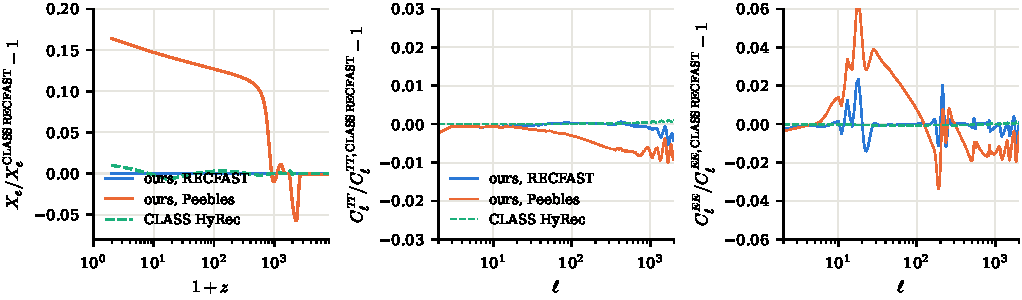
\includegraphics[width=\textwidth]{recfast}
\caption{The RECFAST recombination model. \emph{Left:} $X_e(z)$ without reionization relative to CLASS run with
RECFAST, for our RECFAST (blue) and Peebles (orange) models; the dashed line is CLASS with HyRec. \emph{Middle,
right:} the unlensed TT and EE spectra (with reionization) relative to CLASS RECFAST.}
\label{fig:recfast}
\end{figure*}

% ===========================================================================
\section{Extension: models beyond $\Lambda$CDM}\label{sec:models}
% ===========================================================================

The code has a library of eleven dark-energy and modified-gravity models beyond $\Lambda$CDM (twelve
configurations, since DGP has two branches). This section describes how
a model is organized in the code, the equations of each model, and how it is validated. All models are selected by
name in the parameter file (\texttt{model = ...}), and the model parameters are set there too.

\subsection{Species and gravity}

A model is a list of \emph{species} and a theory of \emph{gravity}. A species provides its background density and
pressure, $\rho(x)$ and $p(x)$, and the first two derivatives of $\rho$. If it clusters, it also has a perturbation
block: its variables, initial conditions and equations. The block is coupled to the metric only through four
moments: $\delta\rho$, $\delta p$, the momentum $(\rho+p)\theta/k$ and the shear $(\rho+p)\sigma$. It receives
$\Phi$, $\Psi$ and $\Phi'$ in return. Interacting components, such as dark matter coupled to dark energy, are a
single block that holds the variables of both. The gravity gives $E^2=H^2/H_0^2$ from the species. It also owns its
own perturbation variables: $\Phi$ in GR, and $\Phi$ plus two scalar-field variables in the scalar--tensor theories.
From these and the summed moments it computes $\Phi$, $\Psi$ and $\Phi'$. Photons and baryons, with Thomson scattering,
tight coupling and the line-of-sight sources, are the fixed core of the perturbation module. All models use the same
conventions as Sec.~\ref{sec:m3}: conformal Newtonian gauge, $x=\ln a$ and our sign of $\Phi$. Below, the spatial
potential is written with the Planck sign, $\Phi_P=-\Phi$.

Every model is tested in its GR/$\Lambda$CDM limit. Where possible we also check the Einstein constraint equations
that the code does not integrate. Some models evolve $\Phi$ with the energy constraint but not the momentum
constraint; in an interacting model the momentum constraint holds only if the exchanged energy and momentum cancel
between the species. We test the growth of structure on sub-horizon scales against independent solutions of the
quasi-static growth equation, and compare with CLASS, hi\_class and CLASS\_EDE where possible. Table~\ref{tab:models}
summarizes the models, and Figs.~\ref{fig:models_de} and \ref{fig:models_mg} show their effects for the parameters
of the table. All other parameters are those of the fiducial model; $\Om_\Lambda$, or the density of the dark-energy
field, is set by closure. The runs use RECFAST and include lensing.

\subsection{Dark energy and dark-sector interactions}

\paragraph*{Quintessence (\texttt{quintessence}).} A minimally coupled scalar field with potential
$V=3H_0^2M_{\rm pl}^2V_0e^{-\lambda\phi}$ (the field $\phi$ is in units of $M_{\rm pl}$). It starts at rest in the
radiation era, where Hubble friction freezes it, and $V_0$ is found by shooting so that the field closes the
universe. With $\phi_x=d\phi/dx$, the background equations are
\begin{equation}
E^2=\frac{\rho_o+v}{1-\phi_x^2/6},\quad
\phi_{xx}=-\Big(3+\frac{d\ln E}{dx}\Big)\phi_x-\frac{3v_\phi}{E^2},
\end{equation}
where $v=V/(3H_0^2M_{\rm pl}^2)$ and $\rho_o$ is the density of the other species. The field perturbation $\delta\phi$
obeys the Klein--Gordon equation of Mukhanov. We evolve $\delta\phi$ and $w=\delta\phi_x-\phi_x\Psi$; the
combination $w$ removes $\Psi'$ from the equation. \emph{Validation:} the background agrees with an independent
integration in cosmic time, and the Poisson and momentum constraints hold to $10^{-7}$ with the field's density and
momentum.

\paragraph*{Coupled quintessence (\texttt{coupled\_quintessence}).} The dark matter particle mass depends on the
field, $m\propto e^{-\beta\phi}$~\cite{Wetterich1995,Amendola2000}. This gives
\begin{equation}
\rho_c'=-(3+\beta\phi_x)\rho_c,\quad
\phi_{xx}=\dots-\frac{3v_\phi}{E^2}+\frac{3\beta\rho_c}{E^2}.
\end{equation}
The dark matter feels a fifth force, which makes its effective gravitational constant $G(1+2\beta^2)$ on small
scales. It also feels a drag term $\propto\beta\phi_xv_c$. \emph{Validation:} an independent integration in cosmic
time with the coupling; the constraint equations, which hold only if the exchange cancels; and the dark matter
growth with fifth force and drag.

\paragraph*{Dark scattering (\texttt{dark\_scattering}).} Elastic scattering between dark matter and a dark-energy
fluid with constant $w$ and sound speed $\hat c_s^2$~\cite{Simpson2010}. The cross section per unit mass is
$\xi=\sigma_D/m_c$. Only momentum is exchanged, with rates $\Gamma_{\rm DE}=ac\xi\rho_c$ and
$\Gamma_c=(1+w)(\rho_{\rm DE}/\rho_c)\Gamma_{\rm DE}$. At early times $\Gamma_{\rm DE}\gg\Hp$, and the
dark-energy velocity is locked to that of the dark matter. \emph{Validation:} the constraints with momentum exchange;
the drag in the growth against two-fluid growth equations ($5\times10^{-4}$); and, for $\xi=0$, the wCDM/$\Lambda$CDM
ratios against CLASS's fluid dark energy (P(k) to $5\times10^{-5}$, TT to $2\times10^{-4}$ for $\ell\le800$).

\paragraph*{Early dark energy (\texttt{ede}).} An axion-like field with
$V=m^2f^2(1-\cos\phi/f)^n$~\cite{Poulin2019,Smith2020}, plus a cosmological constant. The field is frozen at
$\theta_i=\phi_i/f$ until $H\sim m$. It then oscillates, and its energy dilutes as $a^{-6n/(n+1)}$. The model is
specified as in CLASS\_EDE~\cite{Hill2020}, by the maximum fraction $f_{\rm EDE}$ of the total density, its
redshift $z_c$, $\theta_i$ and $n$. A Newton iteration on $(\ln m^2f^2,\ln f)$ finds the potential, and $\Om_\Lambda$
follows from closure. For $n\le2$ the oscillating field does not dilute faster than radiation, so its fraction does
not peak and $(f_{\rm EDE},z_c)$ do not define the model; the code rejects these cases. The background and the
perturbations are integrated through all oscillations, with the Klein--Gordon equations of quintessence. Both
models share one scalar-field class. A run takes about 90\,s instead of 65\,s for $\Lambda$CDM. \emph{Validation:}
the shooting reproduces $f_{\rm EDE}$ and $z_c$ to $10^{-10}$, and the oscillation-averaged dilution is
$a^{-4.50}$ for $n=3$. The constraints hold to $5\times10^{-6}$, and $f_{\rm EDE}\to0$ is $\Lambda$CDM. Compared
with CLASS\_EDE, the decay constant $f$ agrees to $10^{-3}$. The ratios to $\Lambda$CDM agree to $3\times10^{-5}$ in
$P(k)$ for $k\le0.05\hMpc$ ($7\times10^{-4}$ at $0.1\hMpc$) and to $10^{-3}$ in TT.

\paragraph*{Interacting dark energy (\texttt{ide}).} A dark-energy fluid with constant $w$ that exchanges energy
with the dark matter at the rate $Q=\xi H\rho_{\rm DE}$~\cite{Valiviita2008,Gavela2009}. The energy is transferred
along the dark-matter velocity, so the dark matter feels no drag:
\begin{equation}
\rho_{\rm DE}\propto a^{-3(1+w)-\xi},\quad
\rho_c=\frac{1}{a^3}\Big[\Om_c+\xi\Om_{\rm DE}\frac{1-a^{-(3w+\xi)}}{3w+\xi}\Big].
\end{equation}
In the perturbations, $H$ in $Q$ is replaced by the local expansion rate of the dark matter, $\Theta_c/3$. The
dark-energy pressure is transformed to the fluid rest frame with $\rho_{\rm DE}'$ including the transfer.
Momentum conservation then gives
$\theta_{\rm DE}'=\dots+\xi\Hp[\theta_{\rm DE}-\theta_c/(1+w)]$. The early-time instability of these
models~\cite{Valiviita2008} is avoided if the ``doom factor'' $d=\xi/[3(1+w)]$ is negative; the code rejects
$d>0$ and models with $\rho_c<0$ before today. \emph{Validation:} $\rho_c$ against an independent integration
($10^{-14}$); the constraints with energy exchange ($2\times10^{-6}$); and $\xi=0$ against the separate wCDM
implementation of dark scattering (identical). With $\xi=-0.1$ the dark matter loses energy uniformly, so
$\delta_c$ grows faster: $P(k)$ is 1.254 times that of $\Lambda$CDM at $k=0.1\hMpc$.

\subsection{Modified gravity}

\paragraph*{$\mu$--$\Sigma$ (\texttt{musigma}).} The Planck/DES
parameterization~\cite{Planck2018MG,DES2019MG}. It modifies the Poisson equations for the comoving density
$\rho\Delta$ by
\begin{equation}
k^2\Psi=-4\pi Ga^2\mu\,\rho\Delta,\quad k^2(\Phi_P+\Psi)=-8\pi Ga^2\Sigma\,\rho\Delta,
\end{equation}
with $\mu=1+\mu_0\Om_{\rm DE}(a)/\Om_{\rm DE,0}$ and similarly for $\Sigma$. On super-horizon scales,
$\rho\Delta\sim(k/\Hp)^2\delta\rho$, so computing the potentials from $\rho\Delta$ directly would lose all precision
there. We therefore evolve the GR potential of $\rho\Delta$ with an equation derived from energy--momentum
conservation. This equation reduces exactly to GR for $\mu=\Sigma=1$. \emph{Validation:} the potentials against the
algebraic relations, and the growth against an independent solution of the growth equation with $\mu(a)$
($<10^{-4}$).

\paragraph*{DGP (\texttt{dgp}).} The braneworld model~\cite{Dvali2000}. Its background is
$E=\epsilon\sqrt{\Om_{rc}}+\sqrt{\Om_{rc}+\rho/\rho_{c0}}$, on the normal branch ($\epsilon=-1$, with $\Lambda$) or
the self-accelerating branch ($\epsilon=+1$). Optionally the expansion is that of $\Lambda$CDM, as in N-body work.
The perturbations are quasi-static, with $\mu=1+1/(3\beta)$,
$\beta=1-2\epsilon(Hr_c/c)(1+\dot H/3H^2)$, and $\Sigma=1$~\cite{Koyama2006}. They use the $\mu$--$\Sigma$
equations. \emph{Validation:} as for $\mu$--$\Sigma$, with $\mu(a)$ from the background.

\paragraph*{Jordan--Brans--Dicke (\texttt{jbd}).} The scalar field $\phi$ multiplies $R$, with coupling $\omega$,
plus a cosmological constant~\cite{BransDicke1961}. $\phi_0$ is fixed so that the Newtonian constant measured
today is $G$, and $\Om_\Lambda$ follows from $E(0)=1$; both are found by iteration. The perturbations are evolved in
full ($\Phi$, $\delta\phi$, $\delta\phi'$). We derived them symbolically. \emph{Validation:} the background
equations; the matter-era solution $\phi\propto a^{1/(1+\omega)}$; the momentum constraint ($5\times10^{-8}$);
and the growth with $G_{\rm eff}=G\phi_0/\phi$.

\paragraph*{Hu--Sawicky $f(R)$ (\texttt{fr}).} Ref.~\cite{HuSawicki2007} with $f_R=-|f_{R0}|(R_0/R)^{n+1}$. The
expansion is that of $\Lambda$CDM to $\mathcal O(f_{R0})$. The perturbations are quasi-static, with the
scale-dependent
\begin{align}
\mu(k,a)&=\frac{1+4Q}{(1+3Q)(1+f_R)},\quad \Sigma=\frac{1}{1+f_R},\nonumber\\
Q&=\frac{k^2}{a^2}\frac{f_{RR}}{1+f_R}=\frac{k^2\lambda_C^2}{3a^2}.
\end{align}
Below the Compton wavelength of the scalaron, gravity is enhanced by 4/3. \emph{Validation:} $f_R(a)$, the Compton
wavelength and the limits of $\mu$; the potentials at every $k$; and the scale-dependent growth at each $k$
($2\times10^{-4}$).

\paragraph*{Cubic Galileon (\texttt{cubic\_galileon}).} The Lagrangian is $c_2X-g_3X\Box\phi$ on its tracker
solution~\cite{Deffayet2009,Barreira2013}, with $E^2=[\rho+\sqrt{\rho^2+4\Om_\phi}]/2$ and no free parameter beyond
those of $\Lambda$CDM ($w_0\approx-1.19$). The braided scalar perturbations are evolved in full. We derived them
covariantly and checked them with the identity $\nabla^\mu T_{\mu\nu}=(\nabla\cdot J)\phi_\nu$. \emph{Validation:}
the tracker relations ($E^4-\rho E^2=\Om_\phi$, $w=-2/(1+\Om_\phi)$); the momentum constraint with all braiding
terms ($3\times10^{-8}$); and the sub-horizon growth against the quasi-static $G_{\rm eff}$ ($7\times10^{-5}$). The
model is ruled out by the ISW--galaxy cross-correlation. Here it shows the strongest effects: $C_\ell^{\phi\phi}$ is
1.177 times the $\Lambda$CDM value at $\ell=100$.

\paragraph*{Horndeski in the $\alpha$ basis (\texttt{horndeski}).} Following Bellini and Sawicki~\cite{Bellini2014}
and hi\_class~\cite{Zumalacarregui2017}, the linear theory is described by the kineticity $\alpha_K$, the braiding
$\alpha_B$, the running of the Planck mass $\alpha_M=d\ln M_*^2/d\ln a$, and the background. We set $\alpha_T=0$,
as required by GW170817. We derived the Newtonian-gauge equations for $L=F(\phi)R/2+G_2(\phi,X)-G_3(\phi,X)\Box\phi$,
which realizes any $\alpha_K,\alpha_B,\alpha_M$. We then eliminated the functions $G_i$ using the definitions of
the $\alpha$'s, their time derivatives and the background equations, and reduced the system to first order in
$v=-\delta\phi/\phi'$ and $u=v'+\Psi$. The no-ghost and gradient-stability conditions,
\begin{align}
D&=\alpha_K+\tfrac32\alpha_B^2>0,\nonumber\\
Dc_s^2&=(2-\alpha_B)\Big[\frac{\alpha_B}{2}+\alpha_M-\frac{\dot H}{H^2}\Big]\nonumber\\
&\quad-\frac{\rho_m+p_m}{H^2M_*^2}+\frac{\dot\alpha_B}{H}>0,
\end{align}
are checked before a run. The expansion is $\Lambda$CDM or $w_0w_a$. The $\alpha$'s use the hi\_class
parameterizations $\alpha_X=c_X\Om_{\rm DE}(a)$, $c_Xa$ or constant. All terms of the scalar equation are
proportional to an $\alpha$ or to the dark-energy momentum, so nothing cancels catastrophically at early times when
$D\to0$. \emph{Validation:} the momentum constraint ($3\times10^{-8}$). Three theories rebuilt from their $\alpha$'s
reproduce the dedicated implementations: the cubic Galileon ($\alpha_K=6\Om_{\rm DE}$, $\alpha_B=2\Om_{\rm DE}$, to
$5\times10^{-9}$), quintessence ($\alpha_K=3(\rho+p)_\phi/H^2$, $2\times10^{-11}$), and Brans--Dicke on its own
expansion ($M_*^2=\phi$, $\alpha_M=-\alpha_B$, $\alpha_K=\omega\alpha_M^2$, $9\times10^{-9}$). Against hi\_class
the ratios to $\Lambda$CDM agree to $10^{-4}$ in $P(k)$ and $8\times10^{-4}$ in TT.

\begin{table*}
\caption{The models beyond $\Lambda$CDM, the parameters used in Figs.~\ref{fig:models_de}--\ref{fig:models_mg},
the treatment of the perturbations, and $\sigma_8$ and $P(k=0.1\hMpc)$ relative to $\Lambda$CDM (same primordial
spectrum, $\Om_{b}$, $\Om_{c}$ and $h$).}
\label{tab:models}
\begin{ruledtabular}
\begin{tabular}{llllcc}
Model & Parameters & Perturbations & Main validation & $\sigma_8/\sigma_8^{\Lambda\rm CDM}$ & $P/P^{\Lambda\rm CDM}$\\
\hline
quintessence & $\lambda=1$ & full field & constraints, bg. & 0.978 & 0.956\\
coupled quint. & $\lambda=0.5$, $\beta=0.05$ & full field + CDM & constraints, growth & 1.037 & 1.071\\
dark scattering & $w=-0.9$, $\xi=10$\,b/GeV & fluid + CDM & CLASS ($\xi=0$), drag & 0.962 & 0.925\\
EDE & $f_{\rm EDE}=0.12$, $z_c=3630$, $\theta_i=2.83$ & full field & CLASS\_EDE & 0.945 & 0.899\\
IDE & $\xi=-0.1$, $w=-0.95$ & fluid + CDM & constraints, wCDM limit & 1.124 & 1.254\\
$\mu$--$\Sigma$ & $\mu_0=0.3$, $\Sigma_0=0.1$ & $\mu$--$\Sigma$ & growth equation & 1.038 & 1.077\\
nDGP & $H_0r_c/c=1$, $\Lambda$CDM bg. & quasi-static & growth equation & 1.070 & 1.145\\
sDGP & $\Om_\Lambda=0$ & quasi-static & growth equation & 0.809 & 0.654\\
Brans--Dicke & $\omega=100$ & full field & constraints, $G_{\rm eff}$ & 1.043 & 1.093\\
$f(R)$ & $|f_{R0}|=10^{-5}$, $n=1$ & quasi-static $\mu(k,a)$ & scale-dep.\ growth & 1.073 & 1.066\\
cubic Galileon & --- & full field (braiding) & constraints, $G_{\rm eff}$ & 1.097 & 1.203\\
Horndeski & $c_K=1$, $c_B=0.6$, $c_M=0.3$ & full ($\alpha$ basis) & hi\_class, 3 theories & 1.020 & 1.040\\
\end{tabular}
\end{ruledtabular}
\end{table*}

\begin{figure*}
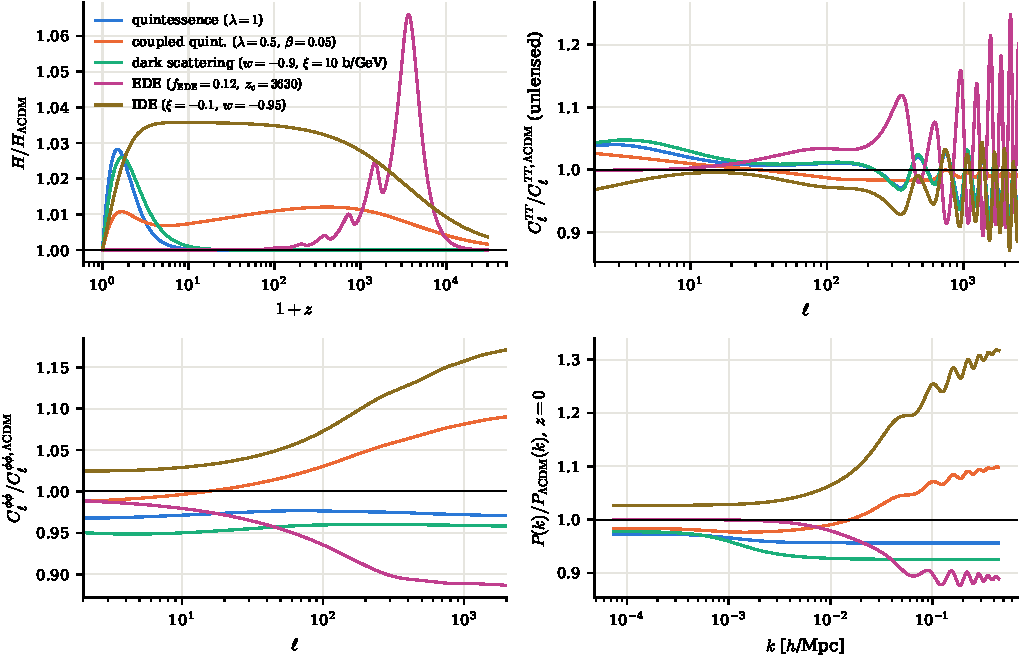
\includegraphics[width=0.85\textwidth]{models_de}
\caption{Dark-energy models and dark-sector interactions relative to $\Lambda$CDM: expansion rate, unlensed TT
spectrum, lensing potential and matter power spectrum today.}
\label{fig:models_de}
\end{figure*}

\begin{figure*}
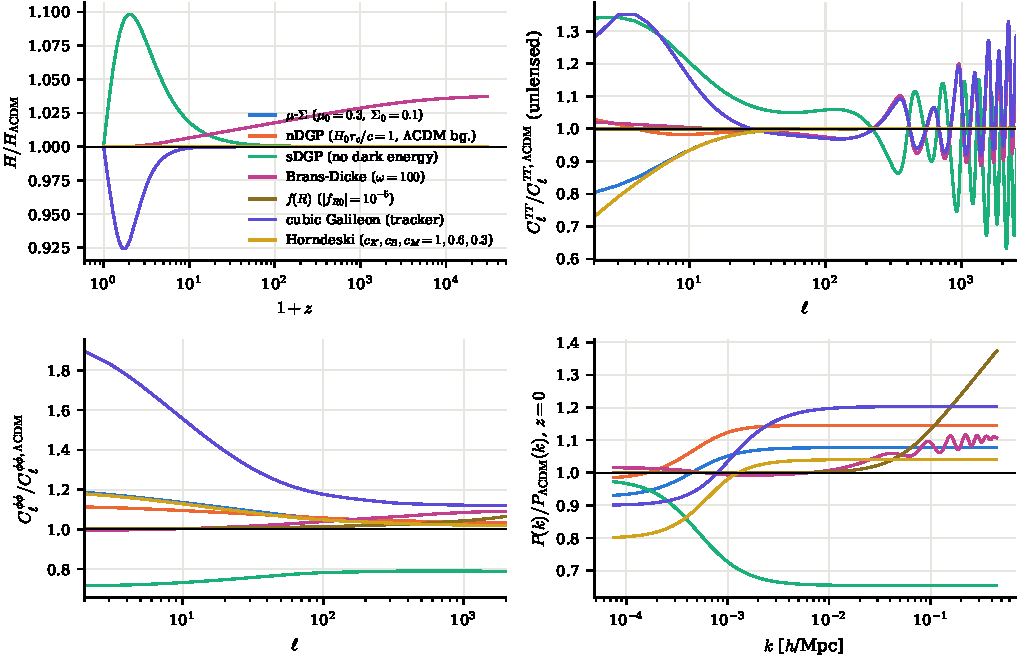
\includegraphics[width=0.85\textwidth]{models_mg}
\caption{Modified-gravity models relative to $\Lambda$CDM, as in Fig.~\ref{fig:models_de}.}
\label{fig:models_mg}
\end{figure*}

\subsection{Discussion}

The models act on the observables in four ways (Figs.~\ref{fig:models_de}--\ref{fig:models_mg},
Table~\ref{tab:models}).
\begin{itemize}
\item \emph{Late-time expansion.} Thawing quintessence raises $H$ at $z\lesssim2$. It slows the growth
      ($\sigma_8$ lower by 2\%) and changes the ISW plateau of TT at $\ell\lesssim20$.
\item \emph{Dark-sector interactions.} These act on the dark matter directly. The fifth force of coupled
      quintessence and the energy outflow of IDE (with $\xi<0$) both enhance the growth of sub-horizon modes, by
      7\% and 25\% in $P(0.1\hMpc)$. IDE also has more
      dark matter in the past, which raises $H$ by about 3\% at high redshift and shifts the acoustic peaks. The drag of
      dark scattering suppresses the growth by 7\% (with $w>-1$).
\item \emph{Modified gravity.} $\mu$--$\Sigma$, nDGP, Brans--Dicke, the Galileon and Horndeski strengthen gravity below
      the horizon. The result is a scale-independent enhancement of $P(k)$ on small scales, between
      4\% (Horndeski) and 20\% (Galileon). $f(R)$ gives
      a scale-dependent enhancement that grows towards the Compton scale. The lensing potential also changes,
      through $\Sigma$ or through the running Planck mass. The self-accelerating DGP branch weakens gravity and
      expands faster, so $P(k)$ is 35\% lower. The scalar--tensor models with dedicated
      field equations also change the large-scale ISW signal of TT strongly: by up to $+35\%$ for the Galileon (at $\ell\approx4$) and
      $-27\%$ for Horndeski (at $\ell=2$).
\item \emph{Early times.} Early dark energy is the only model that acts before recombination. It raises $H$ by up to
      7\% around $z_c$, which reduces the sound horizon. It also slows the growth of the dark matter while the field
      is significant. At fixed $h$ this shifts the acoustic peaks (the ratio to $\Lambda$CDM oscillates by $\pm9\%$), and
      lowers $P(k)$ on small scales by 10\%. In fits to data the smaller sound horizon is
      compensated by a larger $H_0$, which is why the model has been proposed to resolve the Hubble tension.
\end{itemize}
For every model the code computes the unlensed and lensed CMB spectra and the matter power spectrum with the same
pipeline as for $\Lambda$CDM.

% ===========================================================================
\section{Conclusions}\label{sec:conclusions}
% ===========================================================================

We have written a modular Einstein--Boltzmann solver and used it to compute the CMB temperature and polarization
spectra and the matter power spectrum for a flat $\Lambda$CDM model. The four milestones gave:
\begin{enumerate}
\item The background. Radiation--matter equality is at $z=3400$ and acceleration starts at $z=0.63$, before
      matter--$\Lambda$ equality at $z=0.29$, because the negative pressure of $\Lambda$ counts twice in the
      acceleration equation. The Universe is $13.85$\,Gyr old, older than a matter-only universe could be. Supernova
      distances require an accelerating expansion ($\chi^2=31$ versus 317 for a matter-only universe) and prefer
      $h\approx0.70$ when the density parameters are held fixed.
\item The recombination history. The huge number of photons per baryon delays recombination until
      $k_BT\approx\epsilon_0/50$. Photons decouple at $z=1090$, when the Universe is $372\,000$ years old (or at
      $z_*=1085$ including reionization). The baryons, outnumbered by the photons, follow at $z_d=1060$, with sound
      horizon $147\Mpc$. Saha equilibrium ignores the $n=2$ bottleneck and would predict decoupling $\sim200$ units of
      redshift too early and no freeze-out.
\item The perturbations show the main physics of structure formation: acoustic oscillations of the photon--baryon
      fluid, driven by decaying potentials and damped by photon diffusion; the stagnation of dark matter growth in the
      radiation era; baryons falling into dark matter wells after decoupling; the decay of the potentials in the
      $\Lambda$ era; and the brief generation of polarization during decoupling.
\item The spectra reproduce the Planck TT, EE and TE data and the SDSS galaxy power spectrum without any fitting. The
      CMB peaks are the acoustic oscillations frozen at decoupling and projected over $\chi_*$, with spacing set by
      $\ell_A=\pi\chi_*/r_s=303$. Their heights encode the baryon and matter densities, and the turnover of $P(k)$ at
      $k_{\rm eq}$ is the memory of radiation--matter equality. The oscillating residuals of the unlensed TT spectrum are
      explained by gravitational lensing: with our lensing module the $\chi^2$ against the 83 Planck high-$\ell$ bins
      falls from 781 to 220, and the lensed spectra and the lensing B modes agree with CLASS.
\end{enumerate}
All modules agree with CLASS at the percent level or better. As an extension, the code also handles open and
closed universes (Sec.~\ref{sec:curvature}), with hyperspherical Bessel functions and the discrete modes of a closed
space; for $-0.2\le\Om_K\le0.2$ it agrees with CLASS as well as in the flat case, and the first acoustic peak
follows the geometric prediction $\ell_{\rm peak}\simeq0.73\,\pi r(\chi_*)/r_s$. With a massive neutrino species
(Sec.~\ref{sec:neutrinos}) the code reproduces the free-streaming suppression of the matter power spectrum,
$\approx-7f_\nu$ on small scales, and of the lensing potential, with the effect of the mass agreeing with CLASS to
$5\times10^{-4}$ in $P(k)$ and $C_\ell^{TT}$.
The two-point functions of Sec.~\ref{sec:twopoint} show the acoustic physics in real space: a shoulder near $1^\circ$
in the CMB temperature correlation, alternating radial and tangential polarization around hot spots, and the BAO
shell at $r_d$ in the matter correlation function and, projected, at $r_d/\chi$ in $w(\theta)$.

The recombination model was the largest remaining physical approximation. With RECFAST (Sec.~\ref{sec:recfast}),
$X_e$ agrees with CLASS's RECFAST to $3.3\times10^{-4}$, and the TT and EE spectra agree to a few
$10^{-3}$ (rms) up to $\ell=2000$, compared with 1--3\% for the Peebles model. The model library of
Sec.~\ref{sec:models} extends the code to eleven dark-energy and modified-gravity models. Each is validated against
its $\Lambda$CDM limit, the unused constraint equations and independent calculations, and against CLASS, hi\_class
and CLASS\_EDE where these apply. Natural next steps are:
\begin{itemize}
\item Nonlinear corrections to $P(k)$ (halofit or HMcode) for weak-lensing and galaxy-clustering predictions, and
      their extension to modified gravity.
\item Horndeski gravity with $\alpha_T\neq0$, and models built directly from the Horndeski functions $G_i(\phi,X)$.
\item Several massive neutrino species with different masses (the code has one), and $B$-mode polarization from
      tensor modes.
\item MCMC parameter estimation with the full code; the MCMC fits of the course project are omitted from this report
      as instructed.
\end{itemize}
The code takes about one minute to run on a laptop, which is fast enough for such exploratory work.

\begin{acknowledgments}
We thank the authors of CLASS for making their code public, which was invaluable for validation. This work used the
GNU Scientific Library, NumPy, SciPy and Matplotlib.
\end{acknowledgments}


\begin{thebibliography}{99}

\bibitem{Seljak1996}
U.~Seljak and M.~Zaldarriaga, Astrophys.\ J.\ \textbf{469}, 437 (1996).

\bibitem{Lewis2000}
A.~Lewis, A.~Challinor, and A.~Lasenby, Astrophys.\ J.\ \textbf{538}, 473 (2000).

\bibitem{Lesgourgues2011}
J.~Lesgourgues, arXiv:1104.2932 (2011).

\bibitem{Blas2011}
D.~Blas, J.~Lesgourgues, and T.~Tram, J.\ Cosmol.\ Astropart.\ Phys.\ \textbf{07}, 034 (2011).

\bibitem{Planck2018params}
Planck Collaboration, N.~Aghanim \textit{et al.}, Astron.\ Astrophys.\ \textbf{641}, A6 (2020).

\bibitem{Planck2018spectra}
Planck Collaboration, N.~Aghanim \textit{et al.}, Astron.\ Astrophys.\ \textbf{641}, A5 (2020).

\bibitem{Callin2006}
P.~Callin, arXiv:astro-ph/0606683 (2006).

\bibitem{Dodelson2003}
S.~Dodelson, \textit{Modern Cosmology} (Academic Press, San Diego, 2003).

\bibitem{Betoule2014}
M.~Betoule \textit{et al.}, Astron.\ Astrophys.\ \textbf{568}, A22 (2014).

\bibitem{Peebles1968}
P.~J.~E.~Peebles, Astrophys.\ J.\ \textbf{153}, 1 (1968).

\bibitem{Lewis2008}
A.~Lewis, Phys.\ Rev.\ D \textbf{78}, 023002 (2008).

\bibitem{Seager1999}
S.~Seager, D.~D.~Sasselov, and D.~Scott, Astrophys.\ J.\ Lett.\ \textbf{523}, L1 (1999).

\bibitem{Ma1995}
C.-P.~Ma and E.~Bertschinger, Astrophys.\ J.\ \textbf{455}, 7 (1995).

\bibitem{Kodama1984}
H.~Kodama and M.~Sasaki, Prog.\ Theor.\ Phys.\ Suppl.\ \textbf{78}, 1 (1984).

\bibitem{Lewis2006}
A.~Lewis and A.~Challinor, Phys.\ Rep.\ \textbf{429}, 1 (2006).

\bibitem{Challinor2005}
A.~Challinor and A.~Lewis, Phys.\ Rev.\ D \textbf{71}, 103010 (2005).

\bibitem{LesgourguesTram2011}
J.~Lesgourgues and T.~Tram, J.\ Cosmol.\ Astropart.\ Phys.\ \textbf{09}, 032 (2011).

\bibitem{LesgourguesPastor2006}
J.~Lesgourgues and S.~Pastor, Phys.\ Rep.\ \textbf{429}, 307 (2006).

\bibitem{HuEisensteinTegmark1998}
W.~Hu, D.~J.~Eisenstein, and M.~Tegmark, Phys.\ Rev.\ Lett.\ \textbf{80}, 5255 (1998).

\bibitem{Filon1929}
L.~N.~G.~Filon, Proc.\ R.\ Soc.\ Edinburgh \textbf{49}, 38 (1929).

\bibitem{EisensteinHu1998}
D.~J.~Eisenstein and W.~Hu, Astrophys.\ J.\ \textbf{496}, 605 (1998).

\bibitem{Limber1953}
D.~N.~Limber, Astrophys.\ J.\ \textbf{117}, 134 (1953).

\bibitem{LoVerde2008}
M.~LoVerde and N.~Afshordi, Phys.\ Rev.\ D \textbf{78}, 123506 (2008).

\bibitem{Komatsu2011}
E.~Komatsu \textit{et al.}, Astrophys.\ J.\ Suppl.\ \textbf{192}, 18 (2011).

\bibitem{Eisenstein2005}
D.~J.~Eisenstein \textit{et al.}, Astrophys.\ J.\ \textbf{633}, 560 (2005).

\bibitem{Reid2010}
B.~A.~Reid \textit{et al.}, Mon.\ Not.\ R.\ Astron.\ Soc.\ \textbf{404}, 60 (2010).

\bibitem{HuSugiyama1995}
W.~Hu and N.~Sugiyama, Astrophys.\ J.\ \textbf{444}, 489 (1995).

\bibitem{Zaldarriaga1995}
M.~Zaldarriaga and D.~D.~Harari, Phys.\ Rev.\ D \textbf{52}, 3276 (1995).

\bibitem{HuSeljak1998}
W.~Hu, U.~Seljak, M.~White, and M.~Zaldarriaga, Phys.\ Rev.\ D \textbf{57}, 3290 (1998).

\bibitem{Lesgourgues2014}
J.~Lesgourgues and T.~Tram, J.\ Cosmol.\ Astropart.\ Phys.\ \textbf{09}, 032 (2014).

\bibitem{Kosowsky1998}
A.~Kosowsky, arXiv:astro-ph/9805173 (1998).

\bibitem{Tram2017}
T.~Tram, Commun.\ Comput.\ Phys.\ \textbf{22}, 852 (2017).


\bibitem{Wong2008}
W.~Y.~Wong, A.~Moss, and D.~Scott, Mon.\ Not.\ R.\ Astron.\ Soc.\ \textbf{386}, 1023 (2008).

\bibitem{RubinoMartin2010}
J.~A.~Rubi\~no-Mart\'in, J.~Chluba, W.~A.~Fendt, and B.~D.~Wandelt, Mon.\ Not.\ R.\ Astron.\ Soc.\ \textbf{403}, 439 (2010).

\bibitem{Pequignot1991}
D.~P\'equignot, P.~Petitjean, and C.~Boisson, Astron.\ Astrophys.\ \textbf{251}, 680 (1991).

\bibitem{Verner1996}
D.~A.~Verner and G.~J.~Ferland, Astrophys.\ J.\ Suppl.\ \textbf{103}, 467 (1996).

\bibitem{Wetterich1995}
C.~Wetterich, Astron.\ Astrophys.\ \textbf{301}, 321 (1995).

\bibitem{Amendola2000}
L.~Amendola, Phys.\ Rev.\ D \textbf{62}, 043511 (2000).

\bibitem{Simpson2010}
F.~Simpson, Phys.\ Rev.\ D \textbf{82}, 083505 (2010).

\bibitem{Poulin2019}
V.~Poulin, T.~L.~Smith, T.~Karwal, and M.~Kamionkowski, Phys.\ Rev.\ Lett.\ \textbf{122}, 221301 (2019).

\bibitem{Smith2020}
T.~L.~Smith, V.~Poulin, and M.~A.~Amin, Phys.\ Rev.\ D \textbf{101}, 063523 (2020).

\bibitem{Hill2020}
J.~C.~Hill, E.~McDonough, M.~W.~Toomey, and S.~Alexander, Phys.\ Rev.\ D \textbf{102}, 043507 (2020).

\bibitem{Valiviita2008}
J.~V\"aliviita, E.~Majerotto, and R.~Maartens, J.\ Cosmol.\ Astropart.\ Phys.\ \textbf{07}, 020 (2008).

\bibitem{Gavela2009}
M.~B.~Gavela, D.~Hern\'andez, L.~Lopez Honorez, O.~Mena, and S.~Rigolin, J.\ Cosmol.\ Astropart.\ Phys.\ \textbf{07}, 034 (2009).

\bibitem{Planck2018MG}
Planck Collaboration, N.~Aghanim \textit{et al.}, Astron.\ Astrophys.\ \textbf{641}, A6 (2020), Sec.~7.4.

\bibitem{DES2019MG}
DES Collaboration, T.~M.~C.~Abbott \textit{et al.}, Phys.\ Rev.\ D \textbf{99}, 123505 (2019).

\bibitem{Dvali2000}
G.~Dvali, G.~Gabadadze, and M.~Porrati, Phys.\ Lett.\ B \textbf{485}, 208 (2000).

\bibitem{Koyama2006}
K.~Koyama and R.~Maartens, J.\ Cosmol.\ Astropart.\ Phys.\ \textbf{01}, 016 (2006).

\bibitem{BransDicke1961}
C.~Brans and R.~H.~Dicke, Phys.\ Rev.\ \textbf{124}, 925 (1961).

\bibitem{HuSawicki2007}
W.~Hu and I.~Sawicki, Phys.\ Rev.\ D \textbf{76}, 064004 (2007).

\bibitem{Deffayet2009}
C.~Deffayet, G.~Esposito-Far\`ese, and A.~Vikman, Phys.\ Rev.\ D \textbf{79}, 084003 (2009).

\bibitem{Barreira2013}
A.~Barreira, B.~Li, C.~M.~Baugh, and S.~Pascoli, Phys.\ Rev.\ D \textbf{86}, 124016 (2012).

\bibitem{Bellini2014}
E.~Bellini and I.~Sawicki, J.\ Cosmol.\ Astropart.\ Phys.\ \textbf{07}, 050 (2014).

\bibitem{Zumalacarregui2017}
M.~Zumalac\'arregui, E.~Bellini, I.~Sawicki, J.~Lesgourgues, and P.~G.~Ferreira, J.\ Cosmol.\ Astropart.\ Phys.\ \textbf{08}, 019 (2017).

\end{thebibliography}


\end{document}
